%\documentclass[draft]{presentation}
\documentclass[]{presentation}


\title{Experimentos Didácticos de Bajo coste para la Enseñanza del Electromagnetismo}
\author[L. D. Angulo]{\small
 	\textbf{L. D. Angulo} 
}

\institute[UGR]{
	\begin{minipage}{3cm}
		\centering
		\href{http://www.ugr.es}{
\includegraphics[width=2.5cm,height=2.5cm]{escudougr.pdf}}
	\end{minipage}
}

\date[2018-06-26]{Dpto. de Electromagnetismo y Física de la Matería\\
                  Universidad de Granada}

\begin{document}
\begin{frame}[plain]
 \titlepage
\end{frame}

\begin{frame}
	\tableofcontents[hideallsubsections]
\end{frame} 

\section{Electronegatividad de materiales y series triboeléctricas}
\subsection{Introducción teórica}
\begin{frame}{Electroafinidad}
Al frotar dos materiales, estos pueden quedar cargados si. \textit{e.g.} al frotar vidrio y seda ó goma y lana, debido al \textbf{efecto triboeléctrico}. El motivo por el cual unos adquieren carga y otros la pierden es que sus átomos tienen distintas \textbf{electroafinidades}.
\begin{figure}
	\centering
	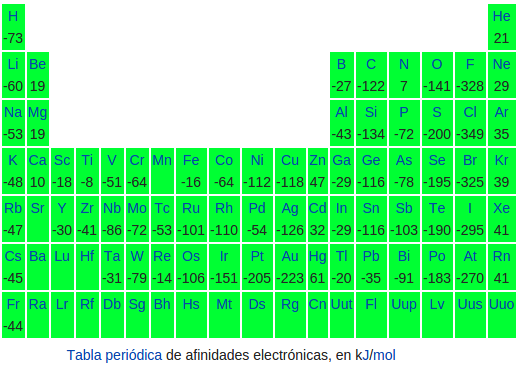
\includegraphics[width=0.7\linewidth]{electroafinica_tabla_periodica}
\end{figure}
\end{frame}

\subsection{Diseño experimental}
\begin{frame}{Materiales}
\begin{figure}
	\centering
	\subfloat[Barra de Nylon (izda, tendencia a adquirir carga positiva) y tubo de PVC (dcha,  tendencia a adquirir carga negativa)]{
		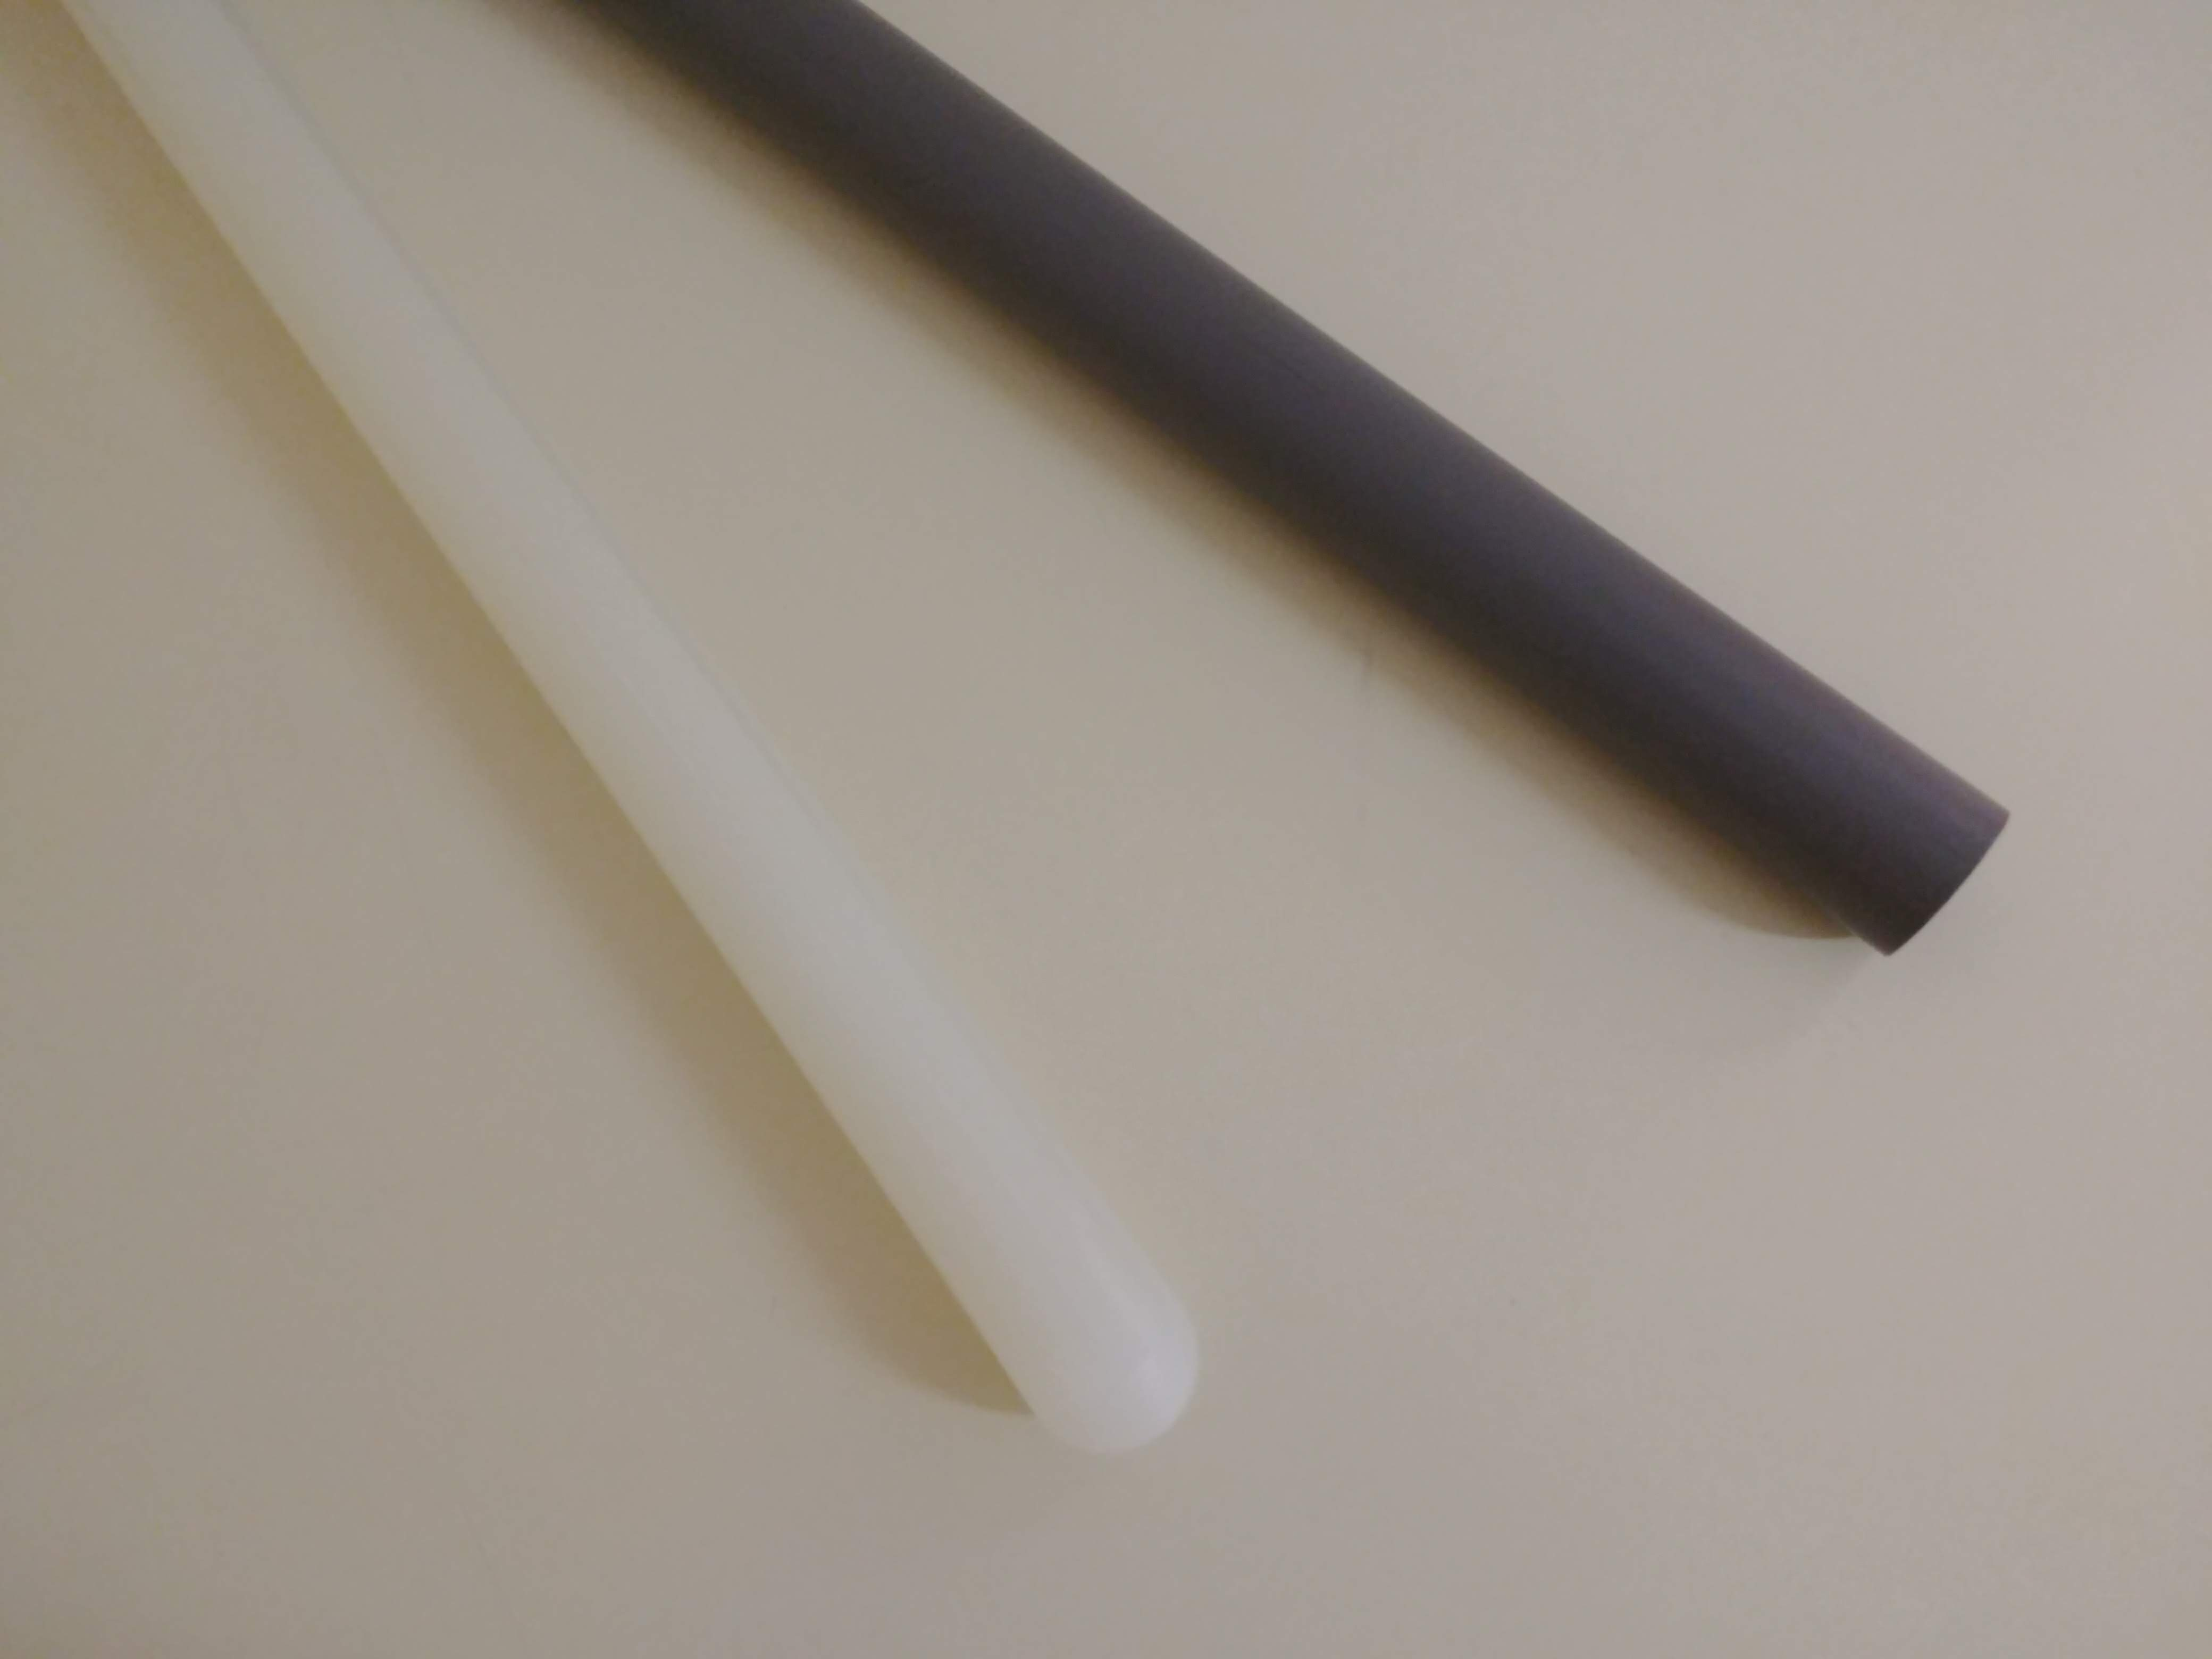
\includegraphics[width=.3\linewidth]{fig/experimentos/triboelectricidad_nylon_pvc}
	}\,
	\subfloat[Paño de cuero (izda, tendencia a adquirir carga positiva) y paño de poliester (dcha,  tendencia a adquirir carga negativa)]{
		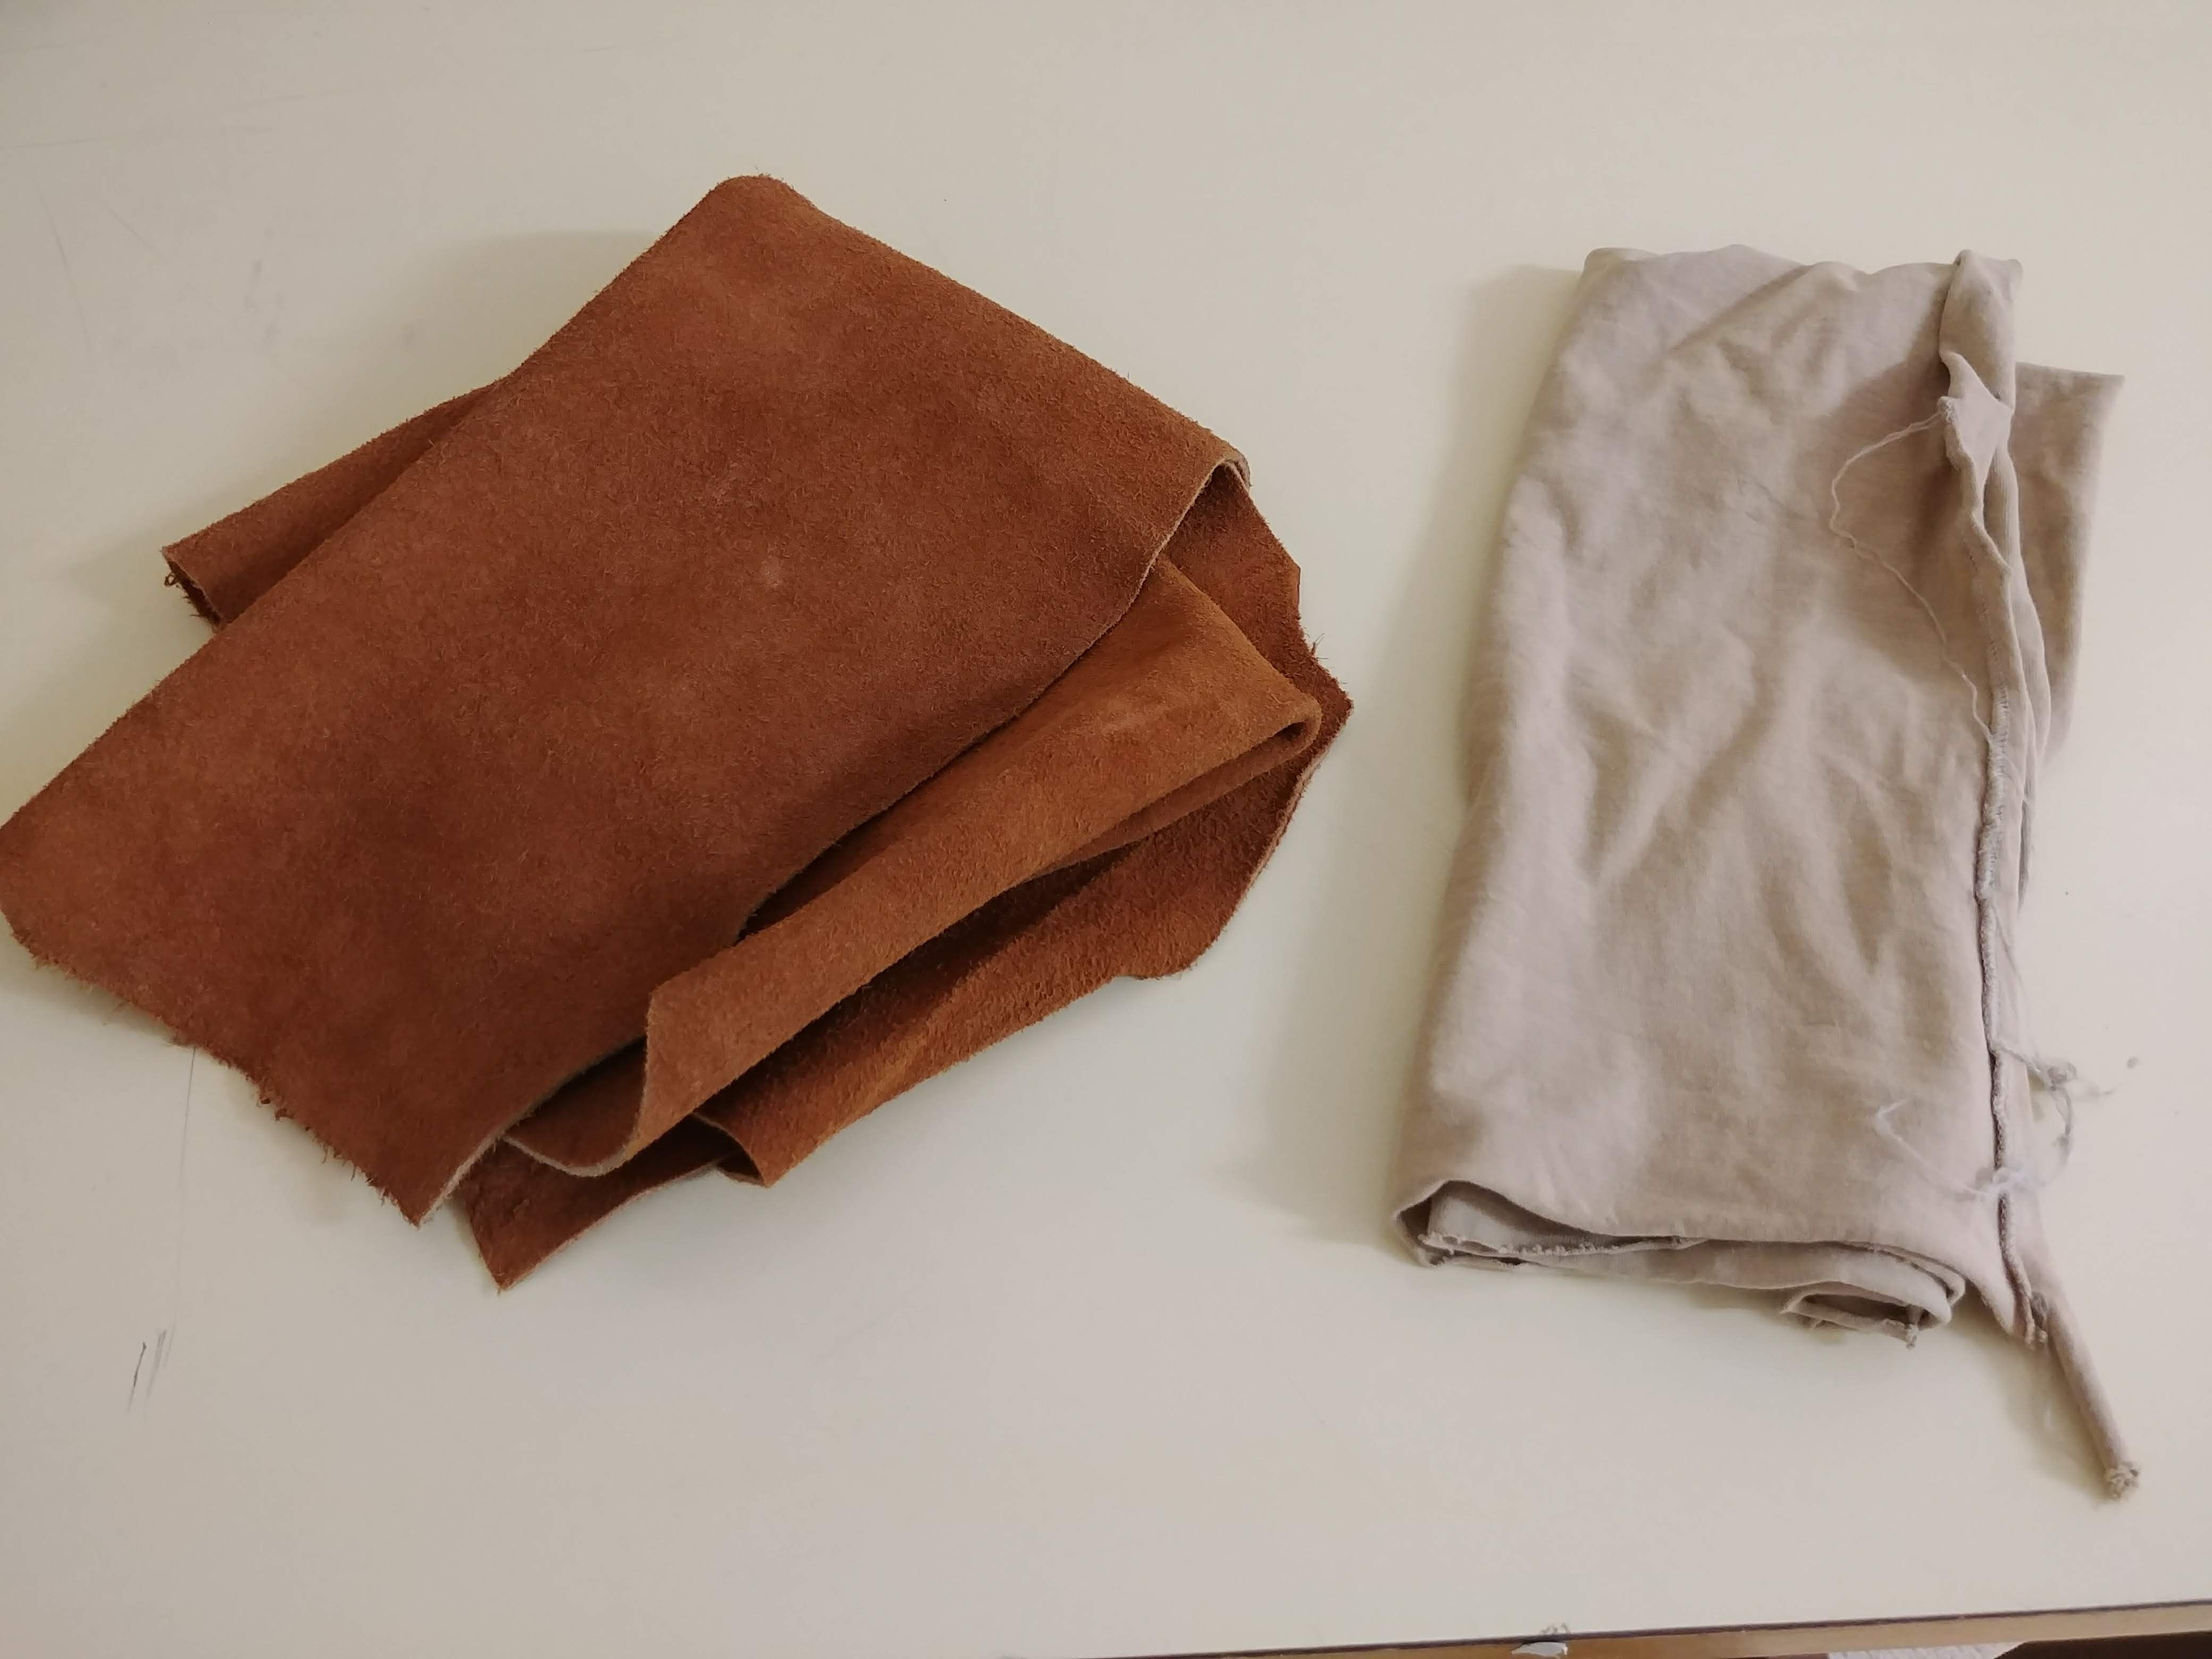
\includegraphics[width=.3\linewidth]{fig/experimentos/triboelectricidad_cuero_poliester}
	}\,
	\subfloat[Papel de aluminio (izda, conductor) y virutas de papel (dcha, no conductor). Ejemplos de materiales conductores y aislantes.]{
		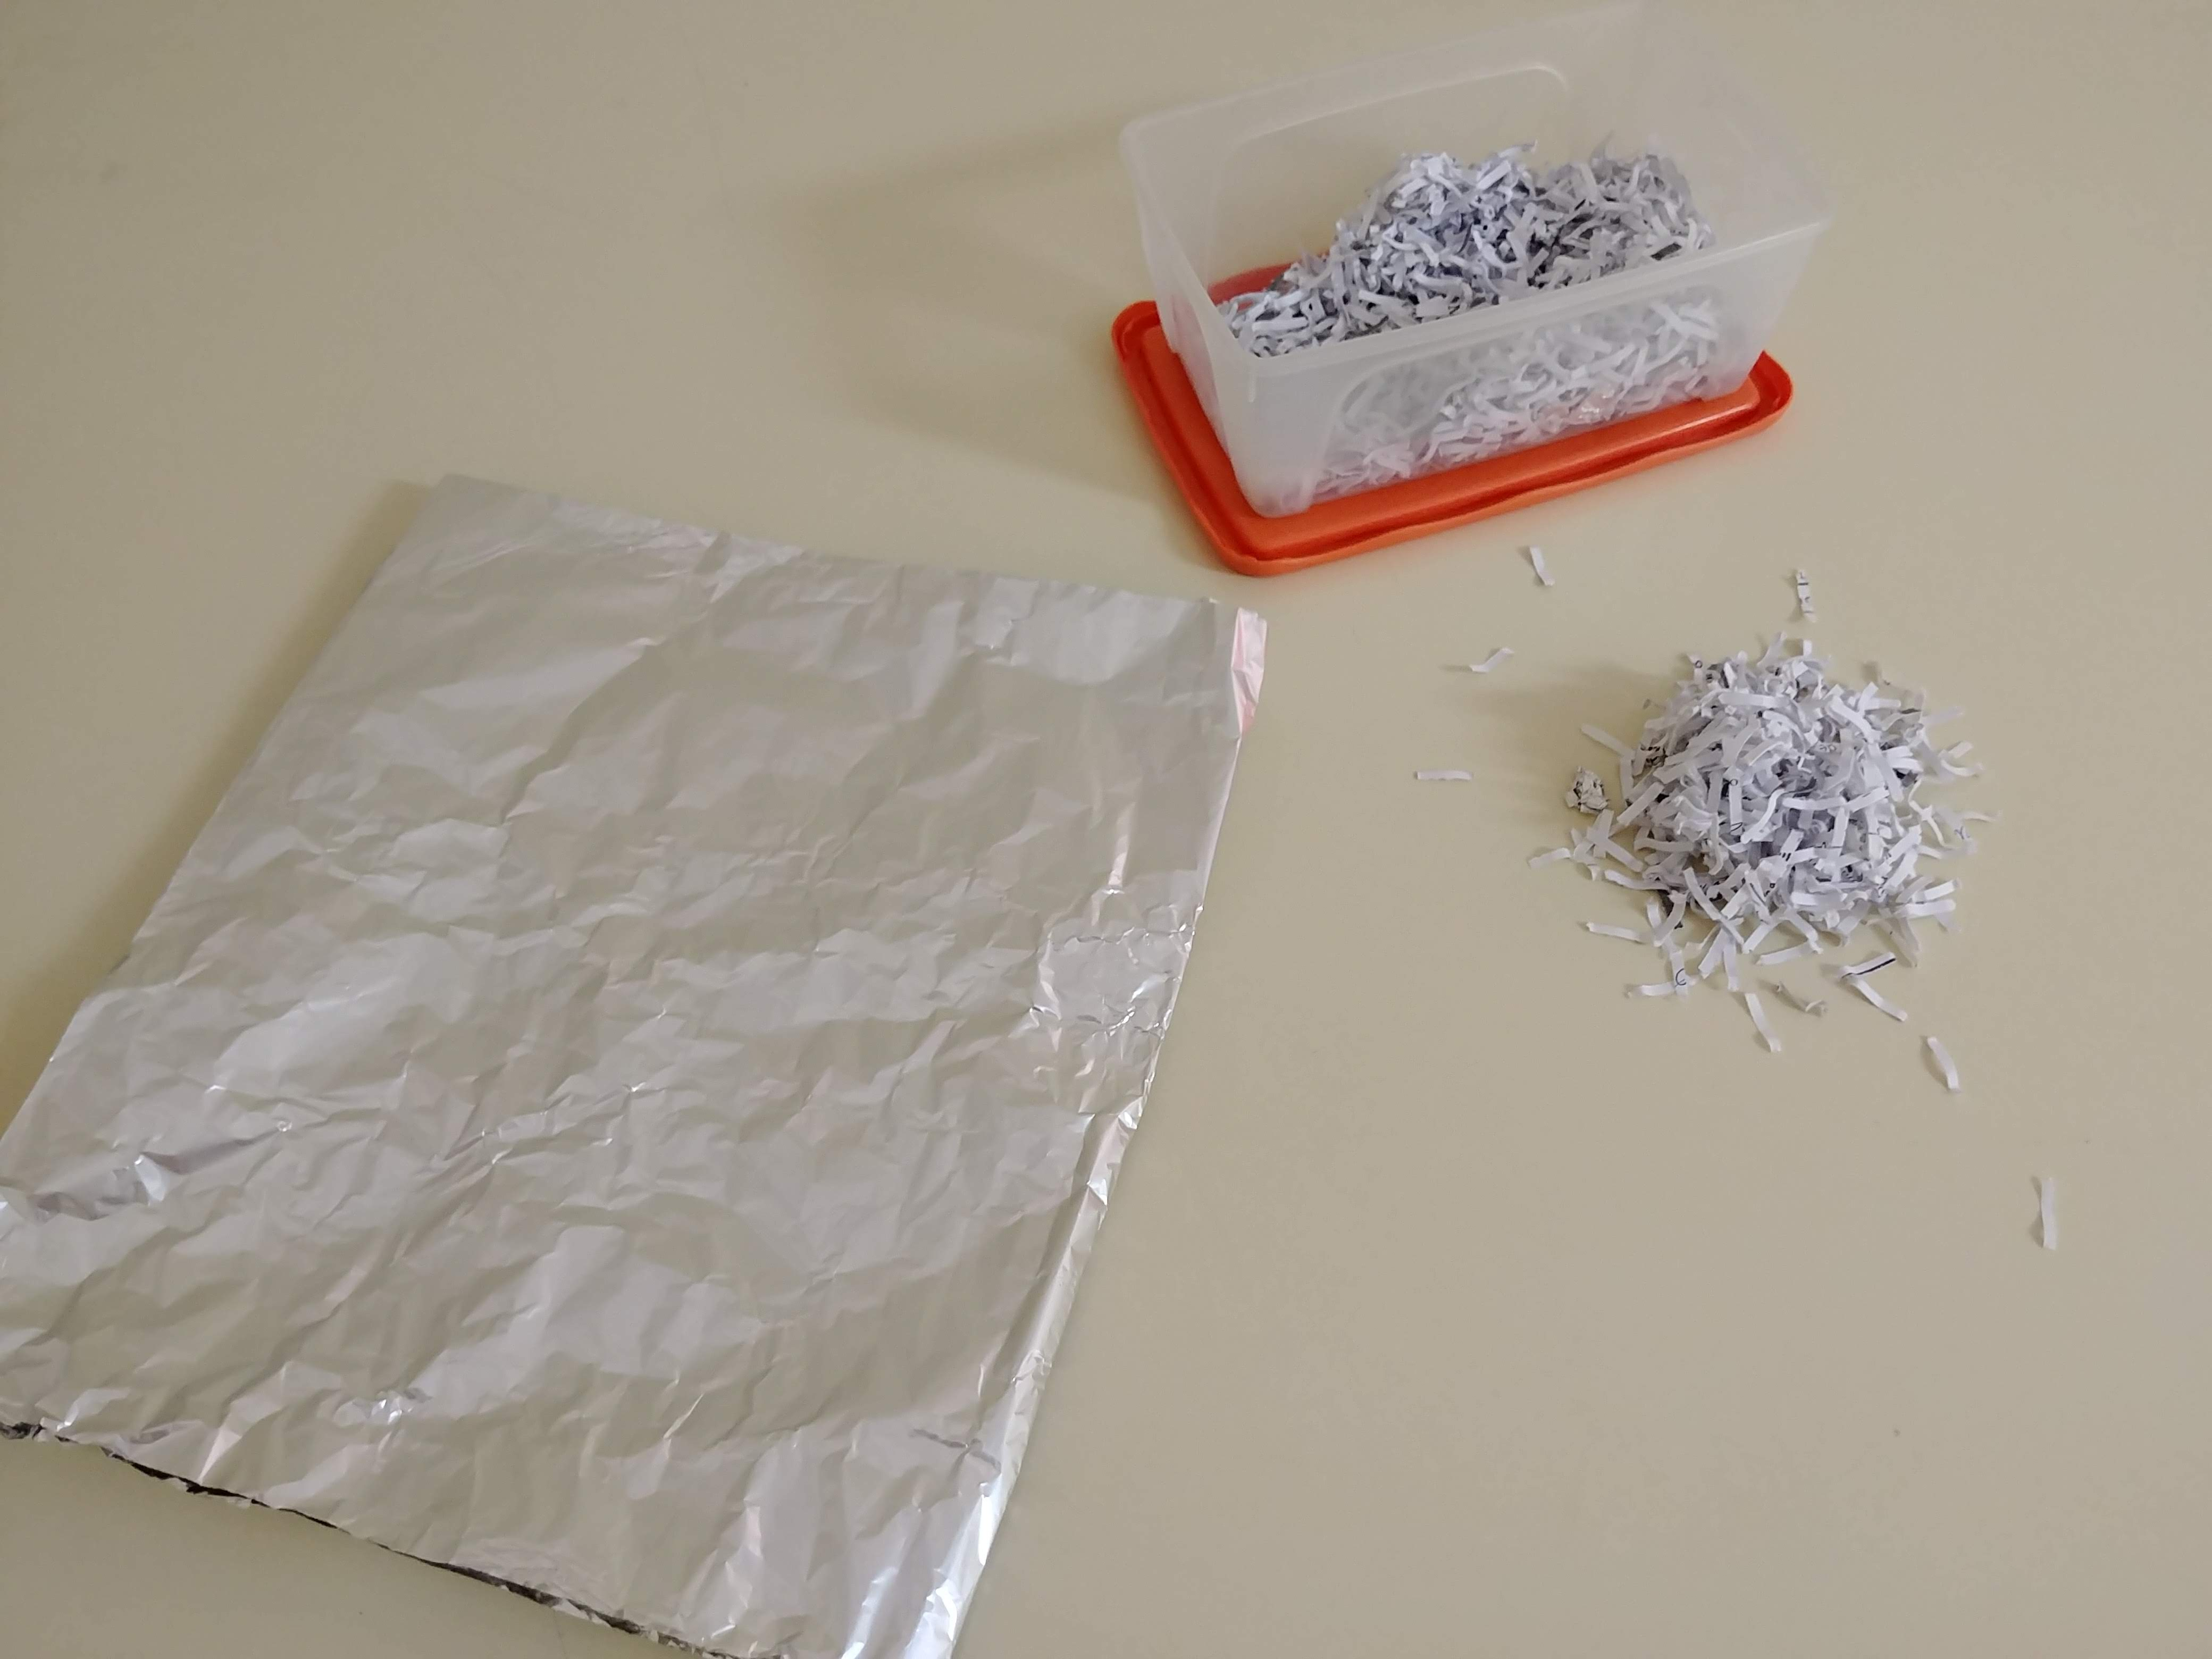
\includegraphics[width=.3\linewidth]{fig/experimentos/triboelectricidad_aluminio_papel}
	}
	\caption{Materiales que adquieren carga mediante efecto triboeléctrico (Figs. (a) y (b). Y materiales que responden de distintas maneras a la presencia de carga (Fig. (c)).}
\end{figure}
\end{frame}

%\subsection{Cuestiones}
%\begin{frame}{Cuestiones}
%	\begin{enumerate}
%		\item 
%		\item 
%	\end{enumerate}
%\end{frame}

\section{Condensadores con elementos caseros}
\subsection{Introducción teórica}
\begin{frame}{Condensadores}
\textbf{Dos conductores separados forman un condensador}. Si cualquiera de los dos conductores empieza a almacenar una carga $Q$, en el otro se almacenará una carga $-Q$; diremos que el condensador tiene carga $Q$ sin especificar el signo. También se establecerá una diferencia de potencial $V$.
\begin{columns}
	\column{0.5\textwidth}      
	\begin{figure}
		\centering
		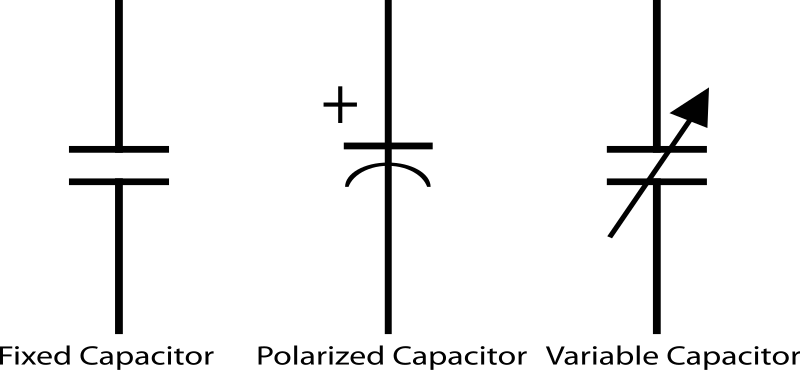
\includegraphics[width=0.6\linewidth]{simbolos_condensadores}
		\caption{Símbolos empleados en diagramas circuitales para representar un condensador}
	\end{figure}
	\column{0.5\textwidth}      
	\begin{figure}
		\centering
		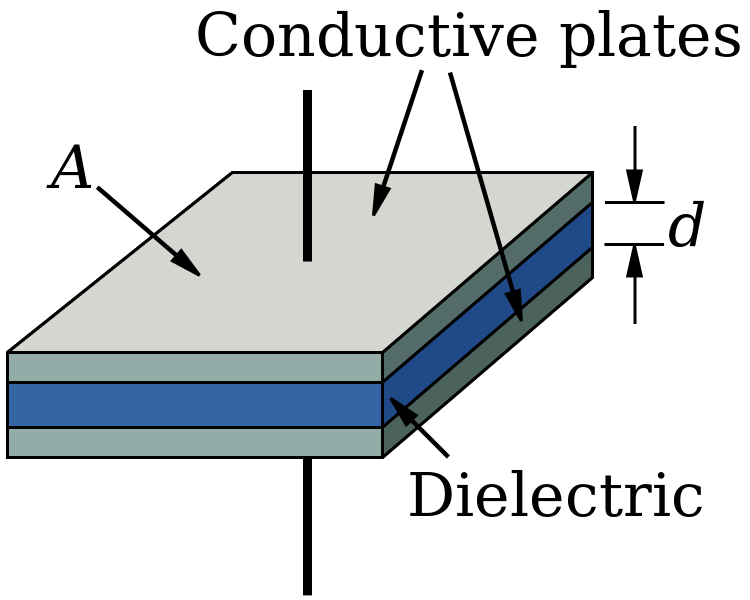
\includegraphics[width=0.6\linewidth]{condensador_placas_planas}
		\caption{Condensador de placas planas y paralelas.}
	\end{figure}
\end{columns}
\end{frame}

\begin{frame}{Capacidad}
\begin{block}{Capacidad}
La capacidad $C$ de un condensador, se define como el cociente entre su carga $Q$ (sin signo) y la diferencia de potencial $V_{ab}$ entre sus conductores
$$
C = \frac{Q}{V} \ \ [\Farad]
$$
\end{block}
Propiedades:
\begin{itemize}
\item Cuanto mayor sea la capacidad $C$ de un condensador, más carga $Q$ podrá almacenar para un potencial dado $V$.
\item El valor de \textbf{la capacidad dependerá unicamente de las formas y tamaños de los conductores y del material que haya entre ambos}.
\end{itemize}
\end{frame}

\begin{frame}{Cálculo de capacidades}
\begin{columns}
\column{0.6\textwidth}      
\begin{exampleblock}{Placas plano-paralelas}
Placas conductoras de area $A$, separadas por una distancia $d$.
\end{exampleblock}
$$
	C = \frac{Q}{V} = \permittivity \frac{A}{d}
$$
\justifying 
Empleando un folio de papel (espesor $d\simeq 0.5\,\mili\meter$) y dos láminas de aluminio de área $A=0.04 \, \meter^2$; obtenemos
$$
	C = 700 \, \pico\Farad
$$
\column{0.4\textwidth}      
\begin{figure}
\centering
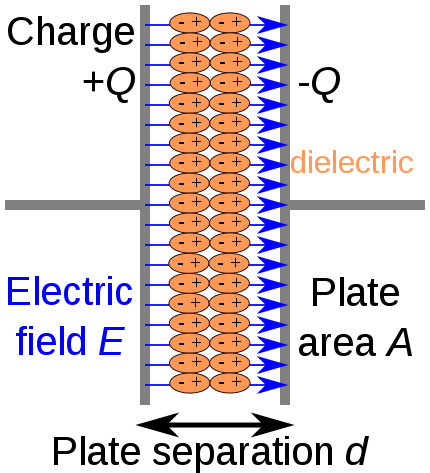
\includegraphics[width=1\linewidth]{condensador_placas_planas_ejemplo}
\caption{\tiny Fuente: Wikipedia, CC BY-SA 3.0}
\end{figure}
\end{columns}
\end{frame}

\begin{frame}
\begin{columns}
	\column{0.5\textwidth}    
	\begin{exampleblock}{Condensador cilíndrico}
		Con radio interior $a$ y exterior $b$; con densidades lineales de carga $+\lambda$ y $-\lambda$; relleno de un dieléctrico $\permittivity$.
	\end{exampleblock}
	\begin{figure}
		\centering
		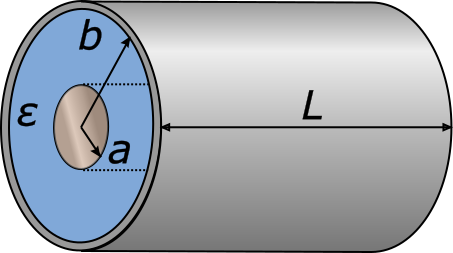
\includegraphics[width=1\linewidth]{condensador_cilindrico}
		\caption{\tiny Fuente: Wikipedia, CC BY-SA 3.0}
	\end{figure}  	
	\column{0.5\textwidth} 
	$$
		C =  \permittivity  \frac{2 \pi L}{\ln(b/a)}
	$$      
	\justifying
	Para una lata de refresco, empleando un hilo de cobre como conductor interno:  $b \simeq 5 \, \centi\meter$, $a \simeq 5 \, \mili\meter$ y $L\simeq 10 \, \centi\meter$.
	$$
		C = 2.4 \, \pico\Farad
	$$
	un valor demasiado pequeño como para ser medido experimentalmente con polímetros normales.
\end{columns}
\end{frame} 

\subsection{Diseño experimental}
\begin{frame}{Materiales}
\begin{figure}
	\centering
	\subfloat[Latas empleadas para desarrollar un condensador cilíndrico. El valor teórico de la capacidad es demasiado pequeño como para ser medido experimentalmente con instrumentos básicos.]{
		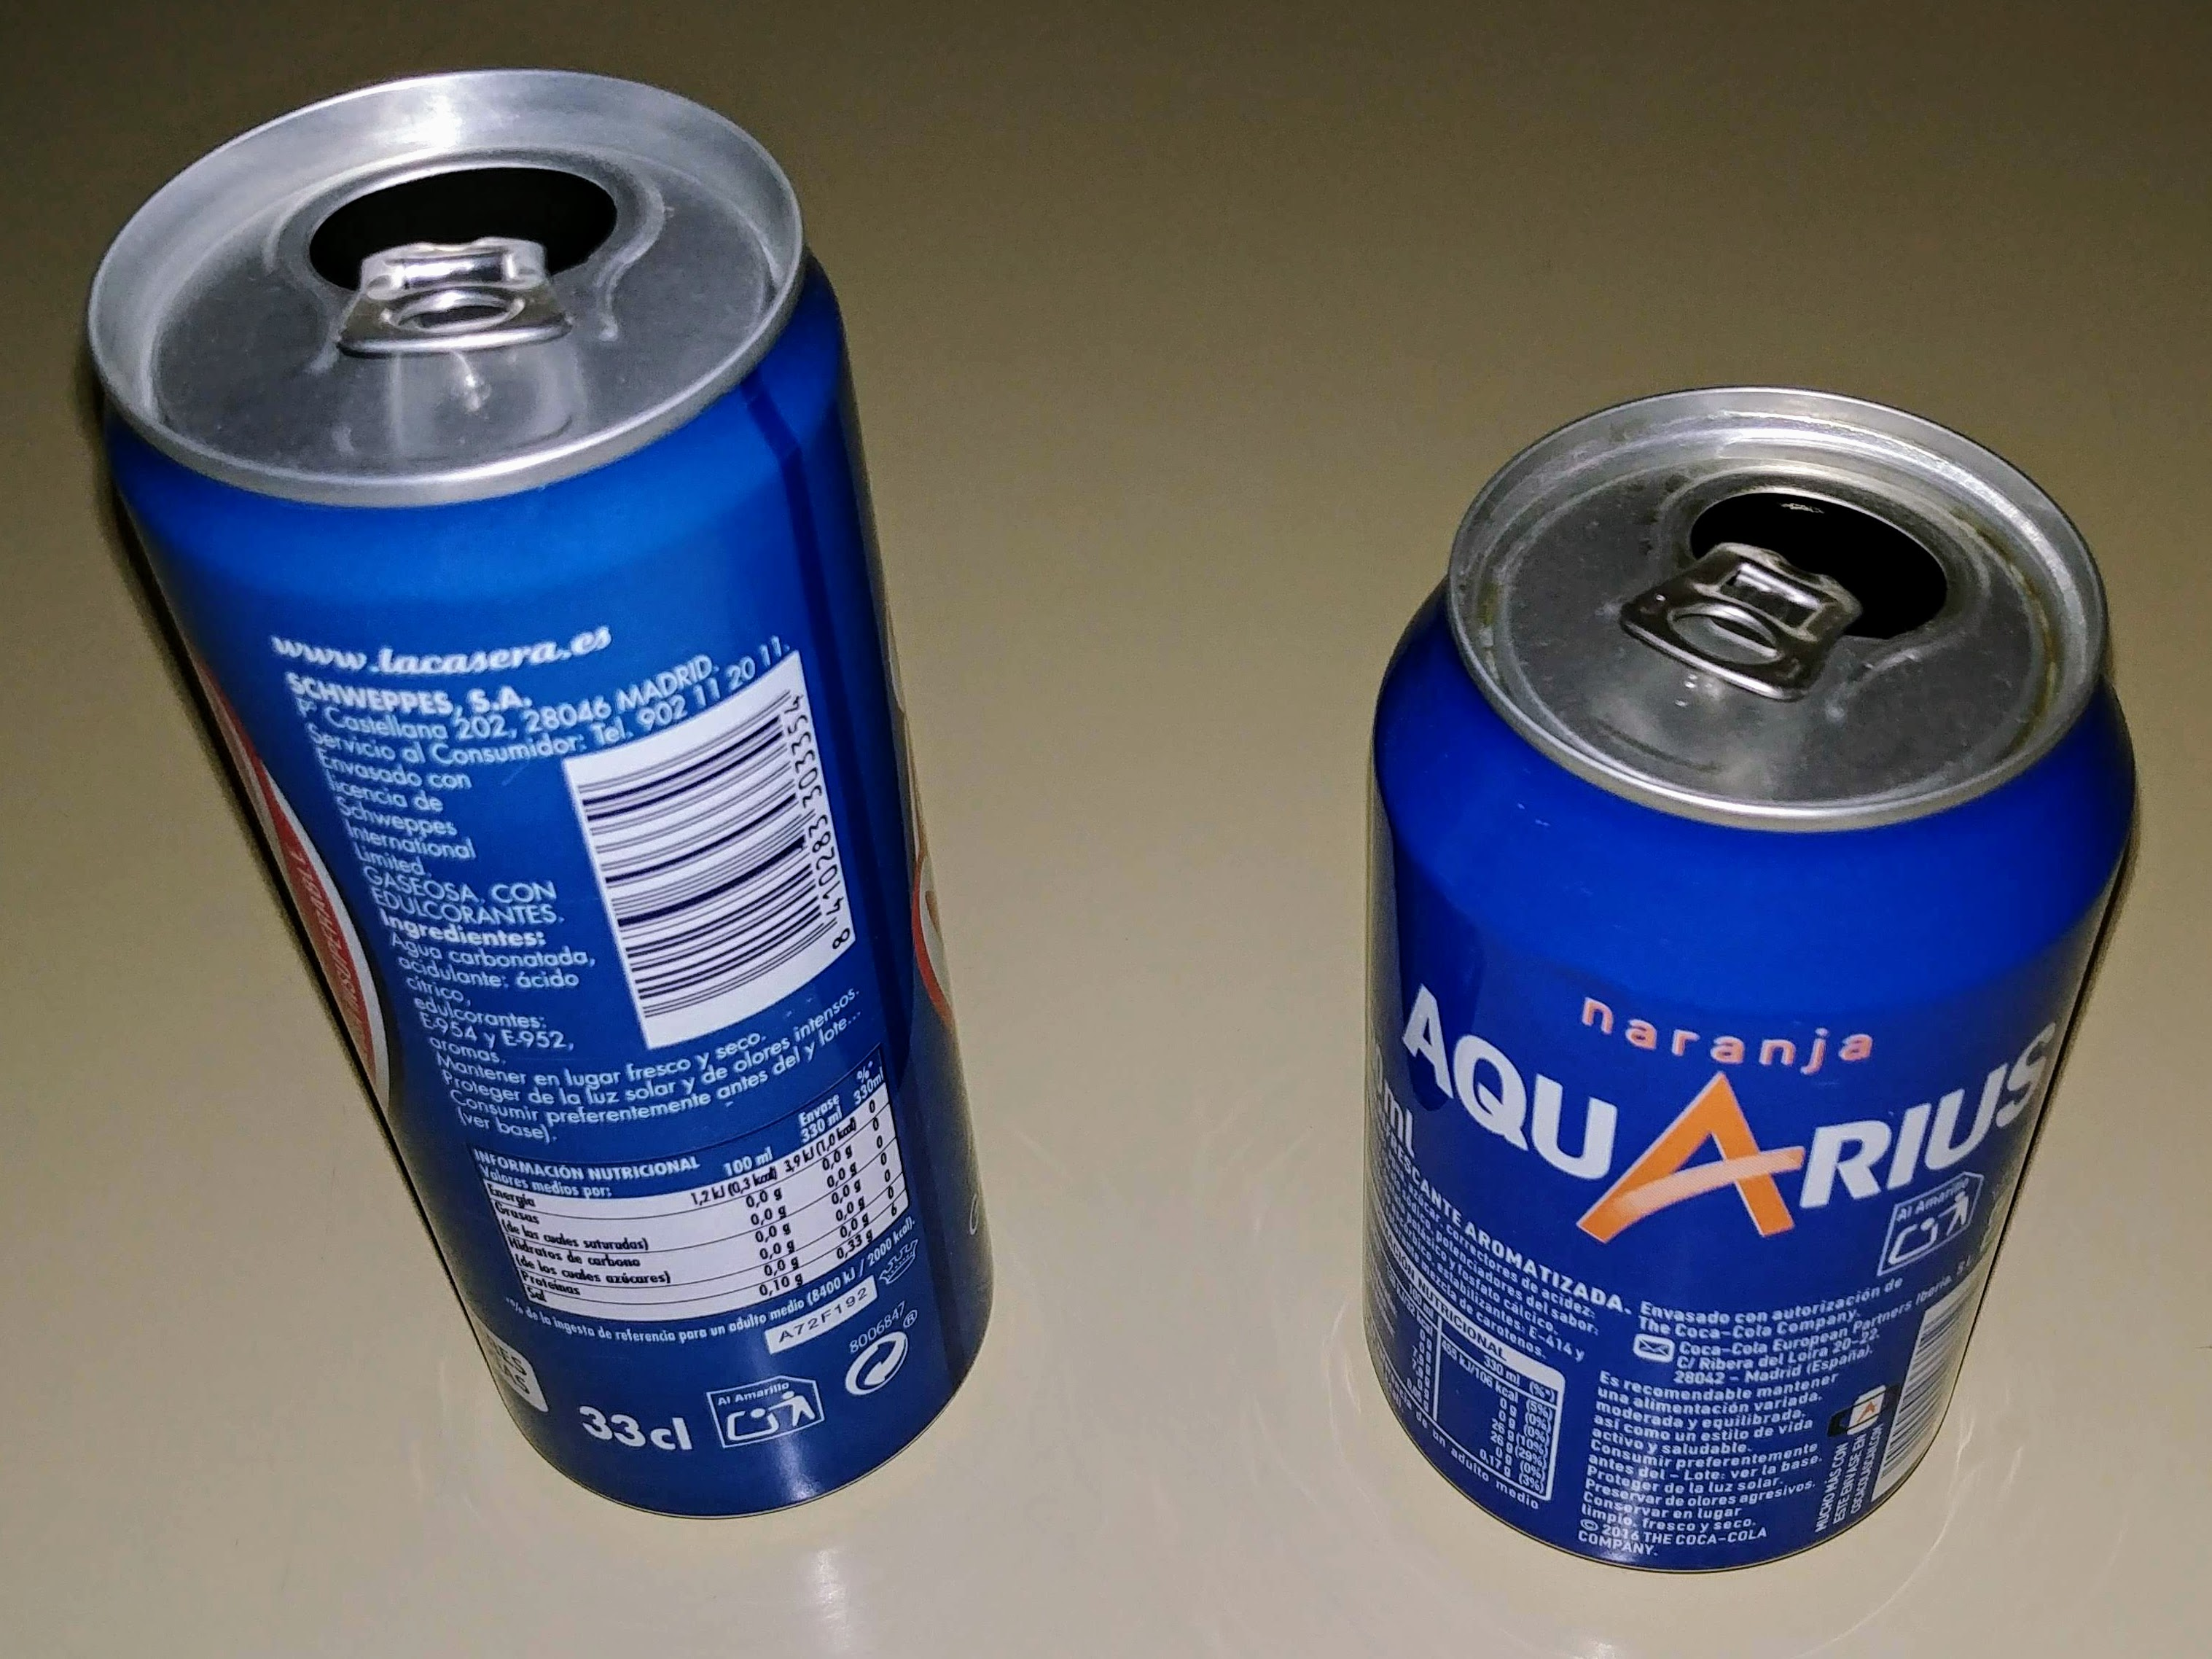
\includegraphics[width=.5\linewidth]{fig/experimentos/latas}
	}\,
	\subfloat[Ejemplo de medida de un condensador de placas plano paralelas hecho con papel de aluminio y empleando una hoja de papel como separador.]{
	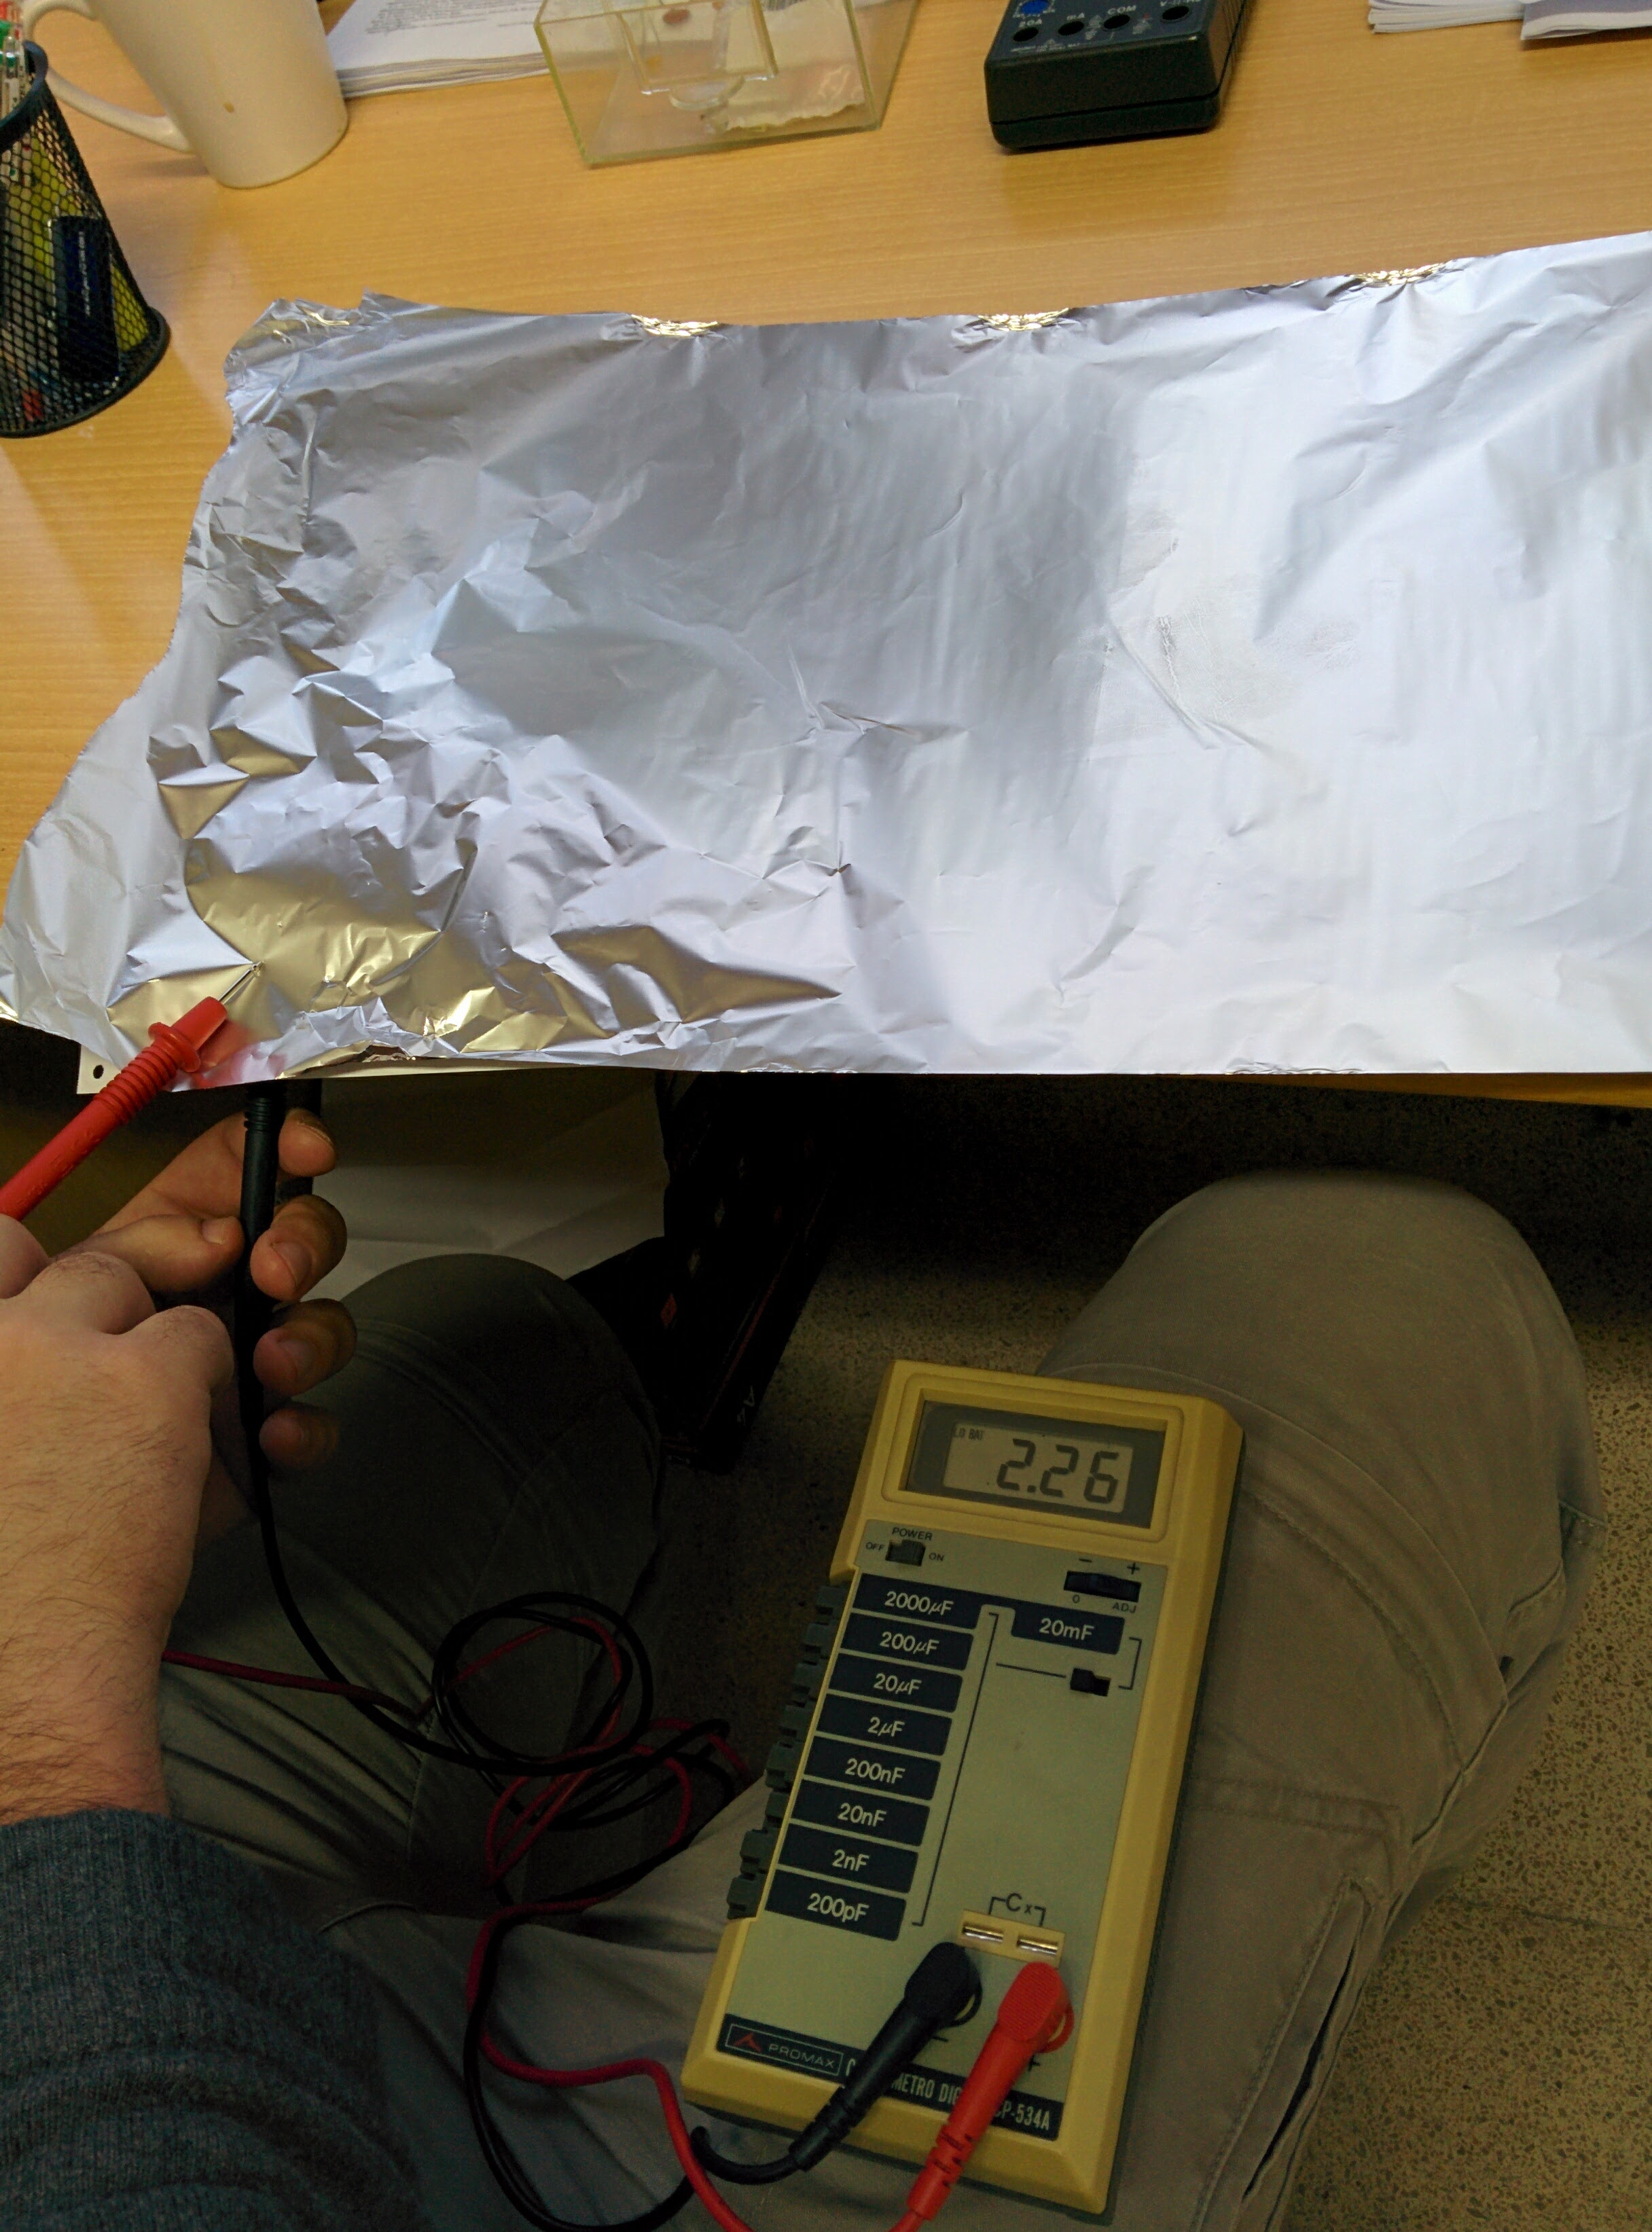
\includegraphics[width=.3\linewidth]{fig/experimentos/condensadores_medida}
	}
\end{figure}
\end{frame}



\section{Visualización de campos magnéticos}
\subsection{Introducción teórica}
\begin{frame}{Campo magnético}
Las interacciones magnéticas se pueden describir mediante un campo magnético,
análogamente a como hemos hecho con el campo eléctrico:
\begin{enumerate}
	\item Una carga en movimiento (corriente) crea un \textbf{campo magnético}, $\magnFlux$, en el espacio que la rodea, además del campo eléctrico debido a su carga.
	\item El campo magnético ejerce una fuerza $\vec{F}$ sobre cualquier carga \textbf{en movimiento} que esté presente en el campo.
\end{enumerate}
\textbf{El campo magnético es un campo vectorial}, la unidad en el SI es el Tesla
$$
[\text{Tesla}] = [\Tesla] = [\Newton \Ampere^{-1} \meter]
$$
Para representar vectores en un plano usaremos el símbolo $\otimes$ cuando se dirijan hacia dentro del plano y $\odot$ cuando se dirijan hacia fuera.   
\end{frame}

\begin{frame}
Las \textbf{líneas de campo magnético} \textbf{no representan líneas de fuerza}, la fuerza dependerá de la velocidad de la particula. Tienen las siguientes características:
\begin{itemize}
\item Las líneas de campo no nacen ni mueren, pasan a través del interior de los imanes.        
\item Apuntan en la dirección que apuntaría una brújula situada en ellas.
\end{itemize}
\begin{columns}
\column{0.3\textwidth}      
\begin{figure}
	\centering
	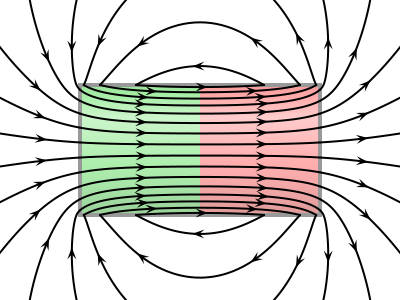
\includegraphics[width=1\linewidth]{lineas_campo_magnetico}
	\caption{\tiny Fuente: Wikipedia, CC BY-SA 3.0}
\end{figure}
\column{0.7\textwidth}
\begin{figure}
	\centering
	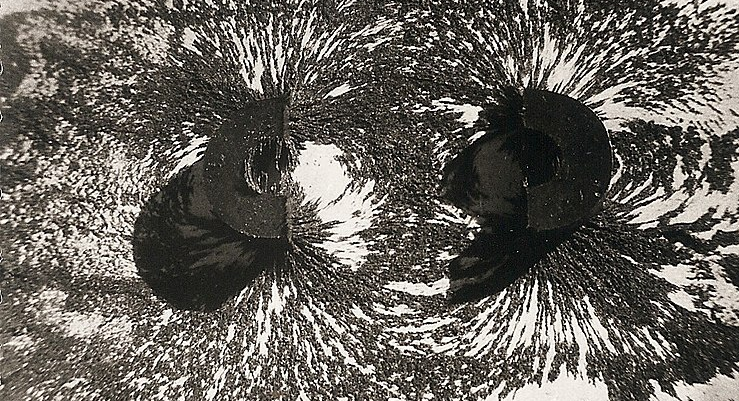
\includegraphics[width=1\linewidth]{limaduras_campo_magnetico}
\end{figure}
\end{columns}
\end{frame}

\subsection{Diseño experimental}
\begin{frame}{Materiales}
\begin{figure}
	\centering
	\subfloat[Campo magnético en limaduras de hierro. Los polos del imán están alineados verticalmente]{
		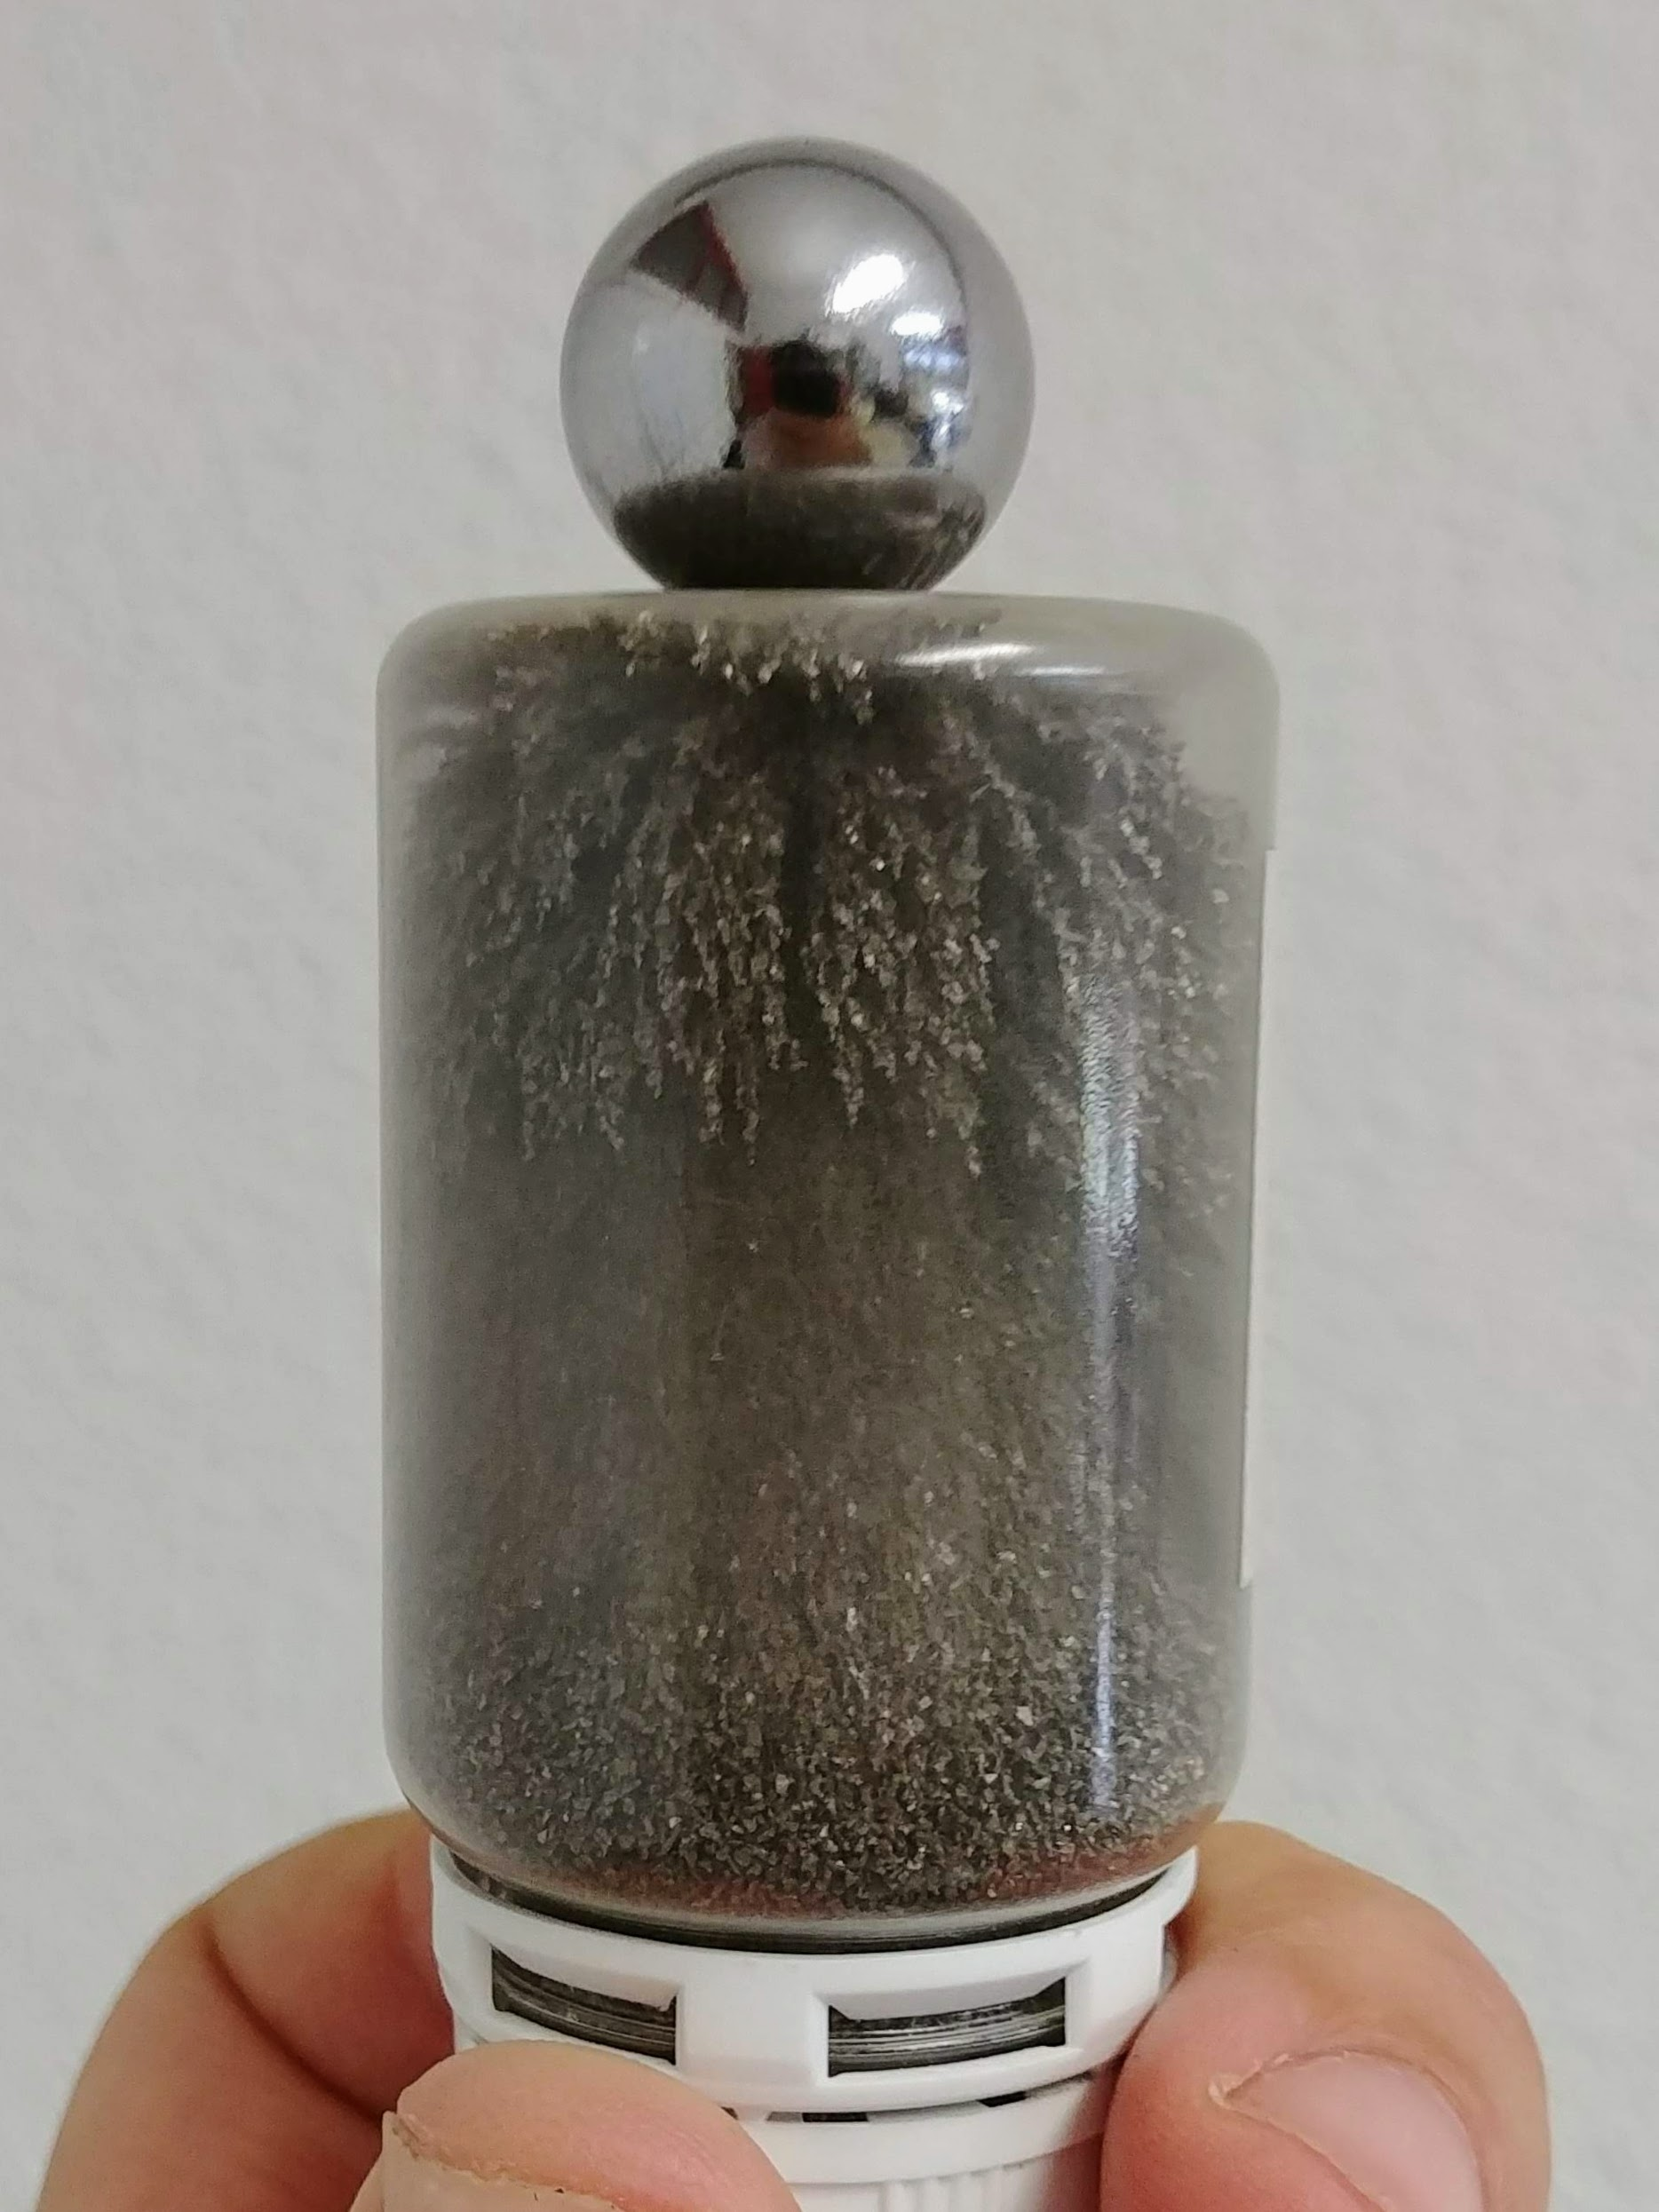
\includegraphics[width=.3\linewidth]{fig/experimentos/visualizacion_limaduras}
	}\,
	\subfloat[Uno de los polos está apuntando hacia la lámina ferrmagnética.]{
		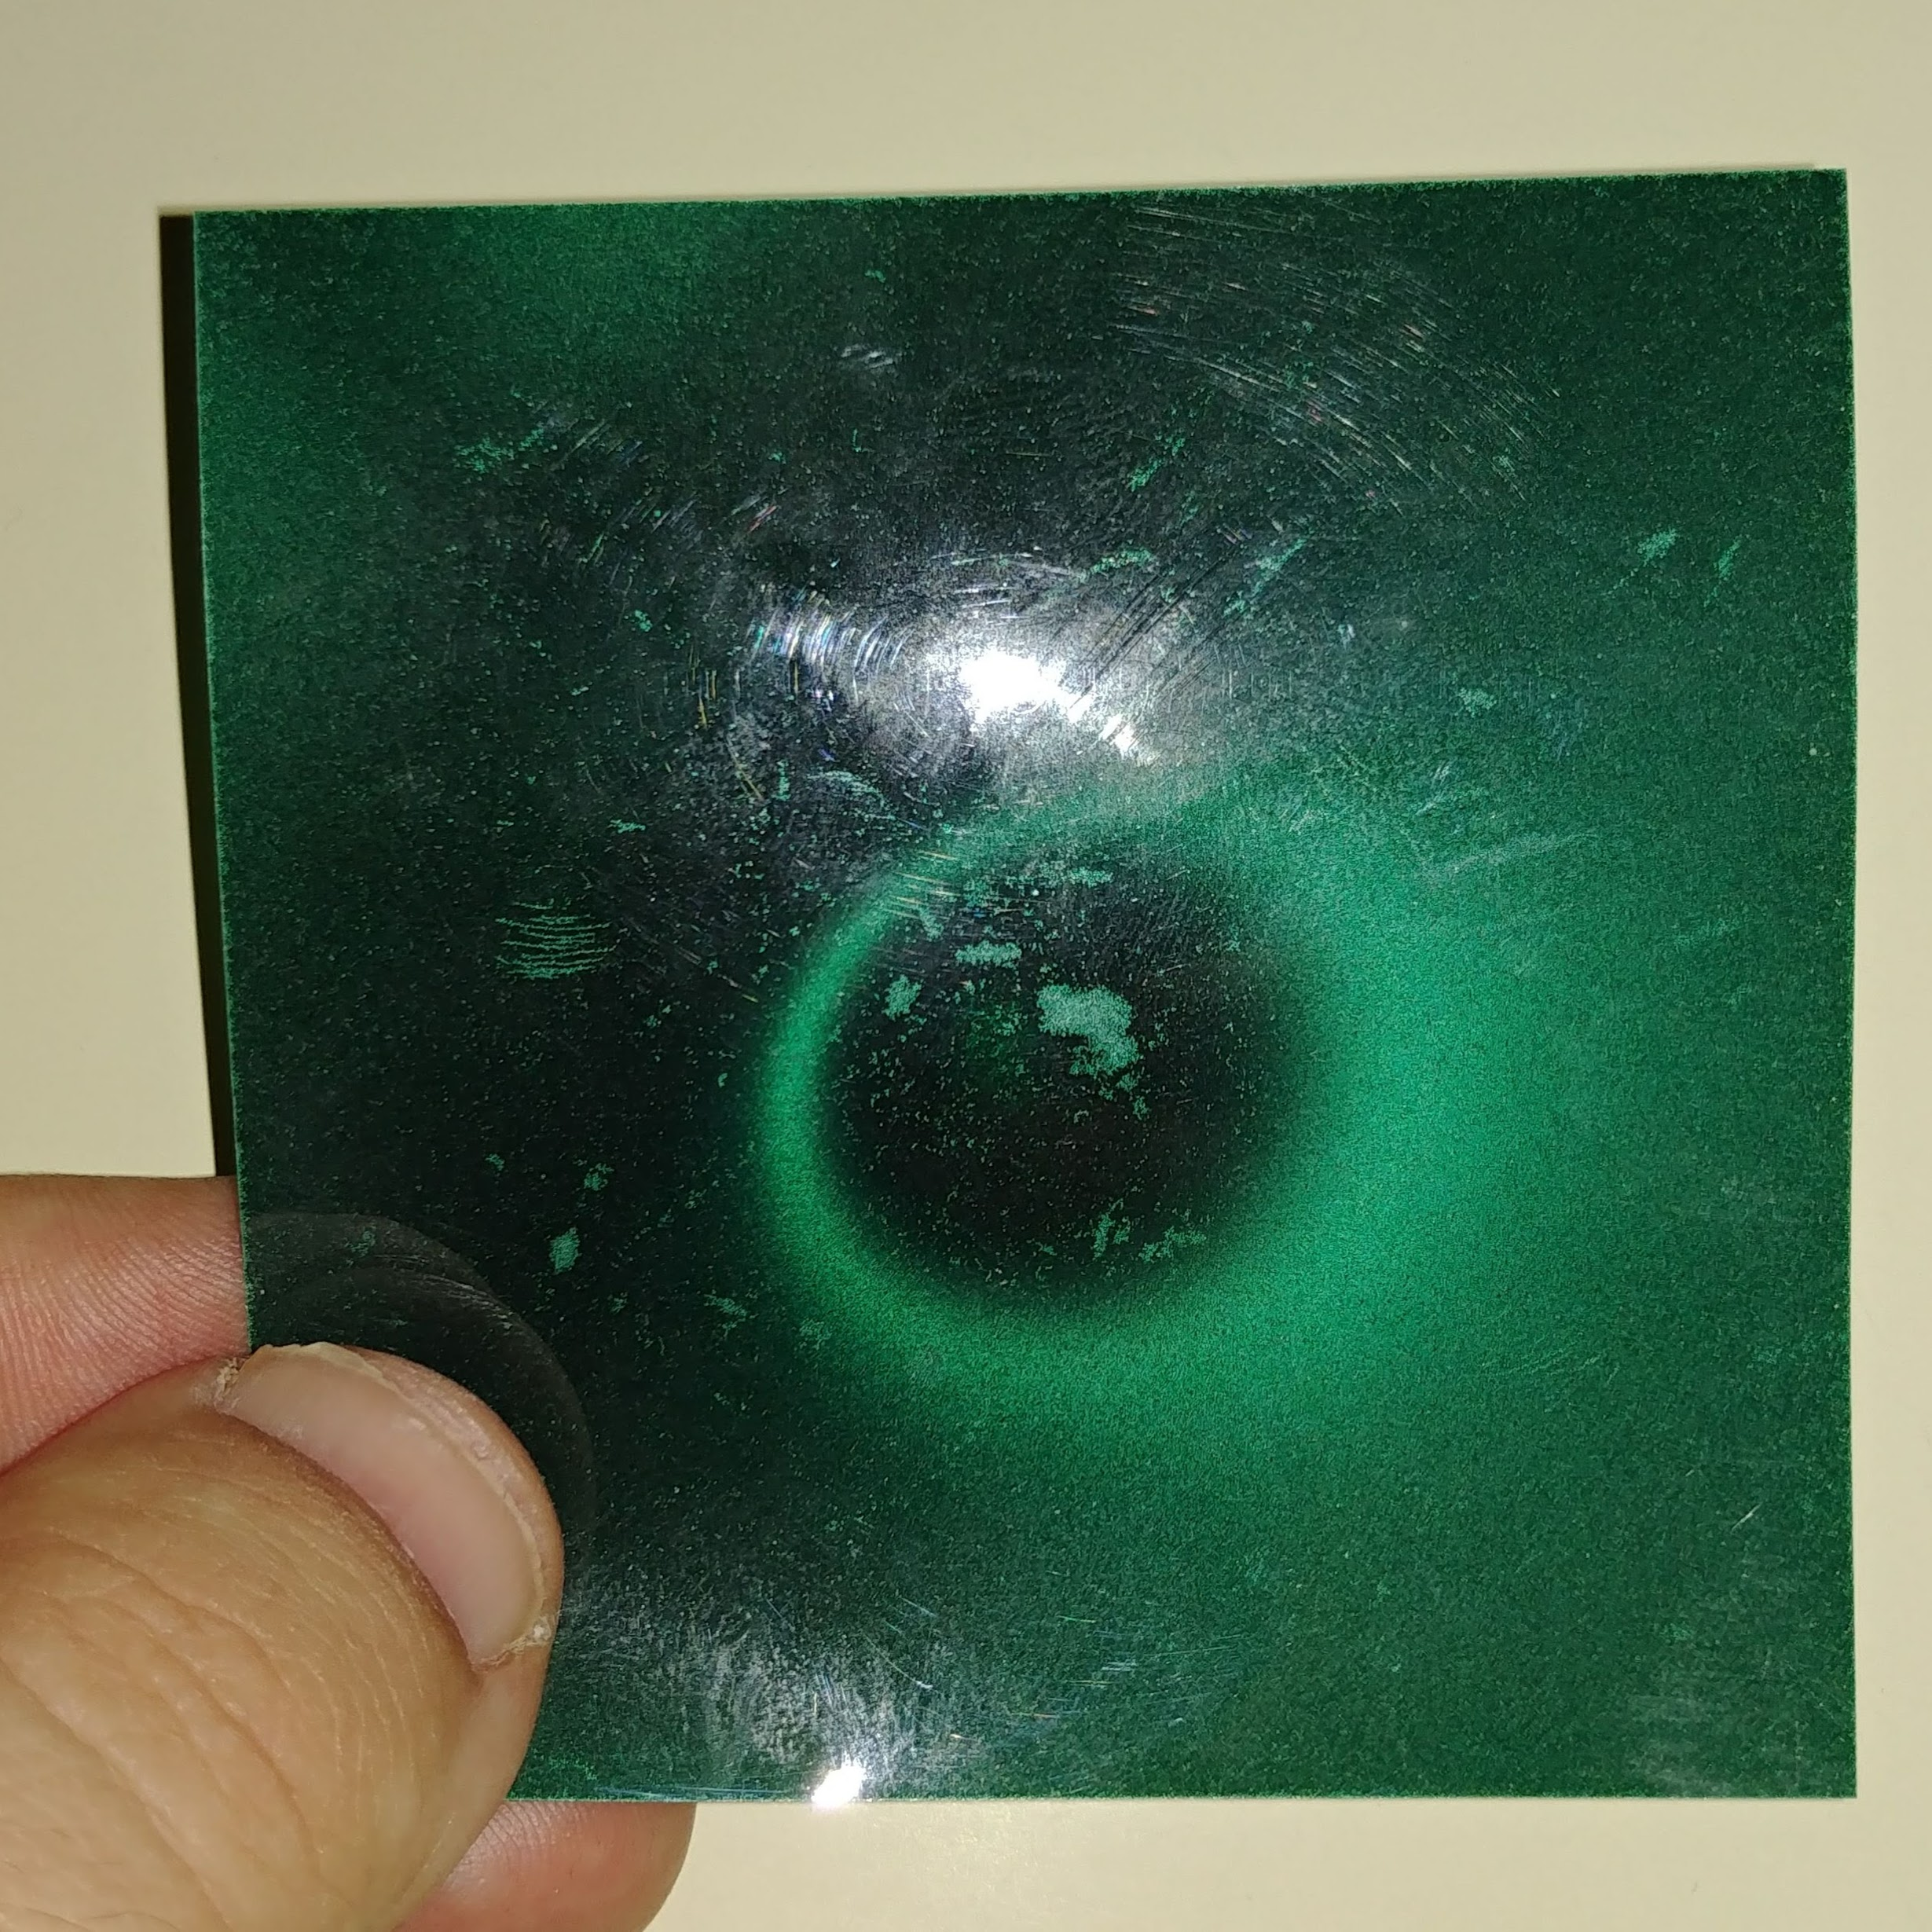
\includegraphics[width=.3\linewidth]{fig/experimentos/visualizacion_B_1}
	}\,
	\subfloat[Ecuador magnético del imán observado empleando la lámina ferromagnética.]{
		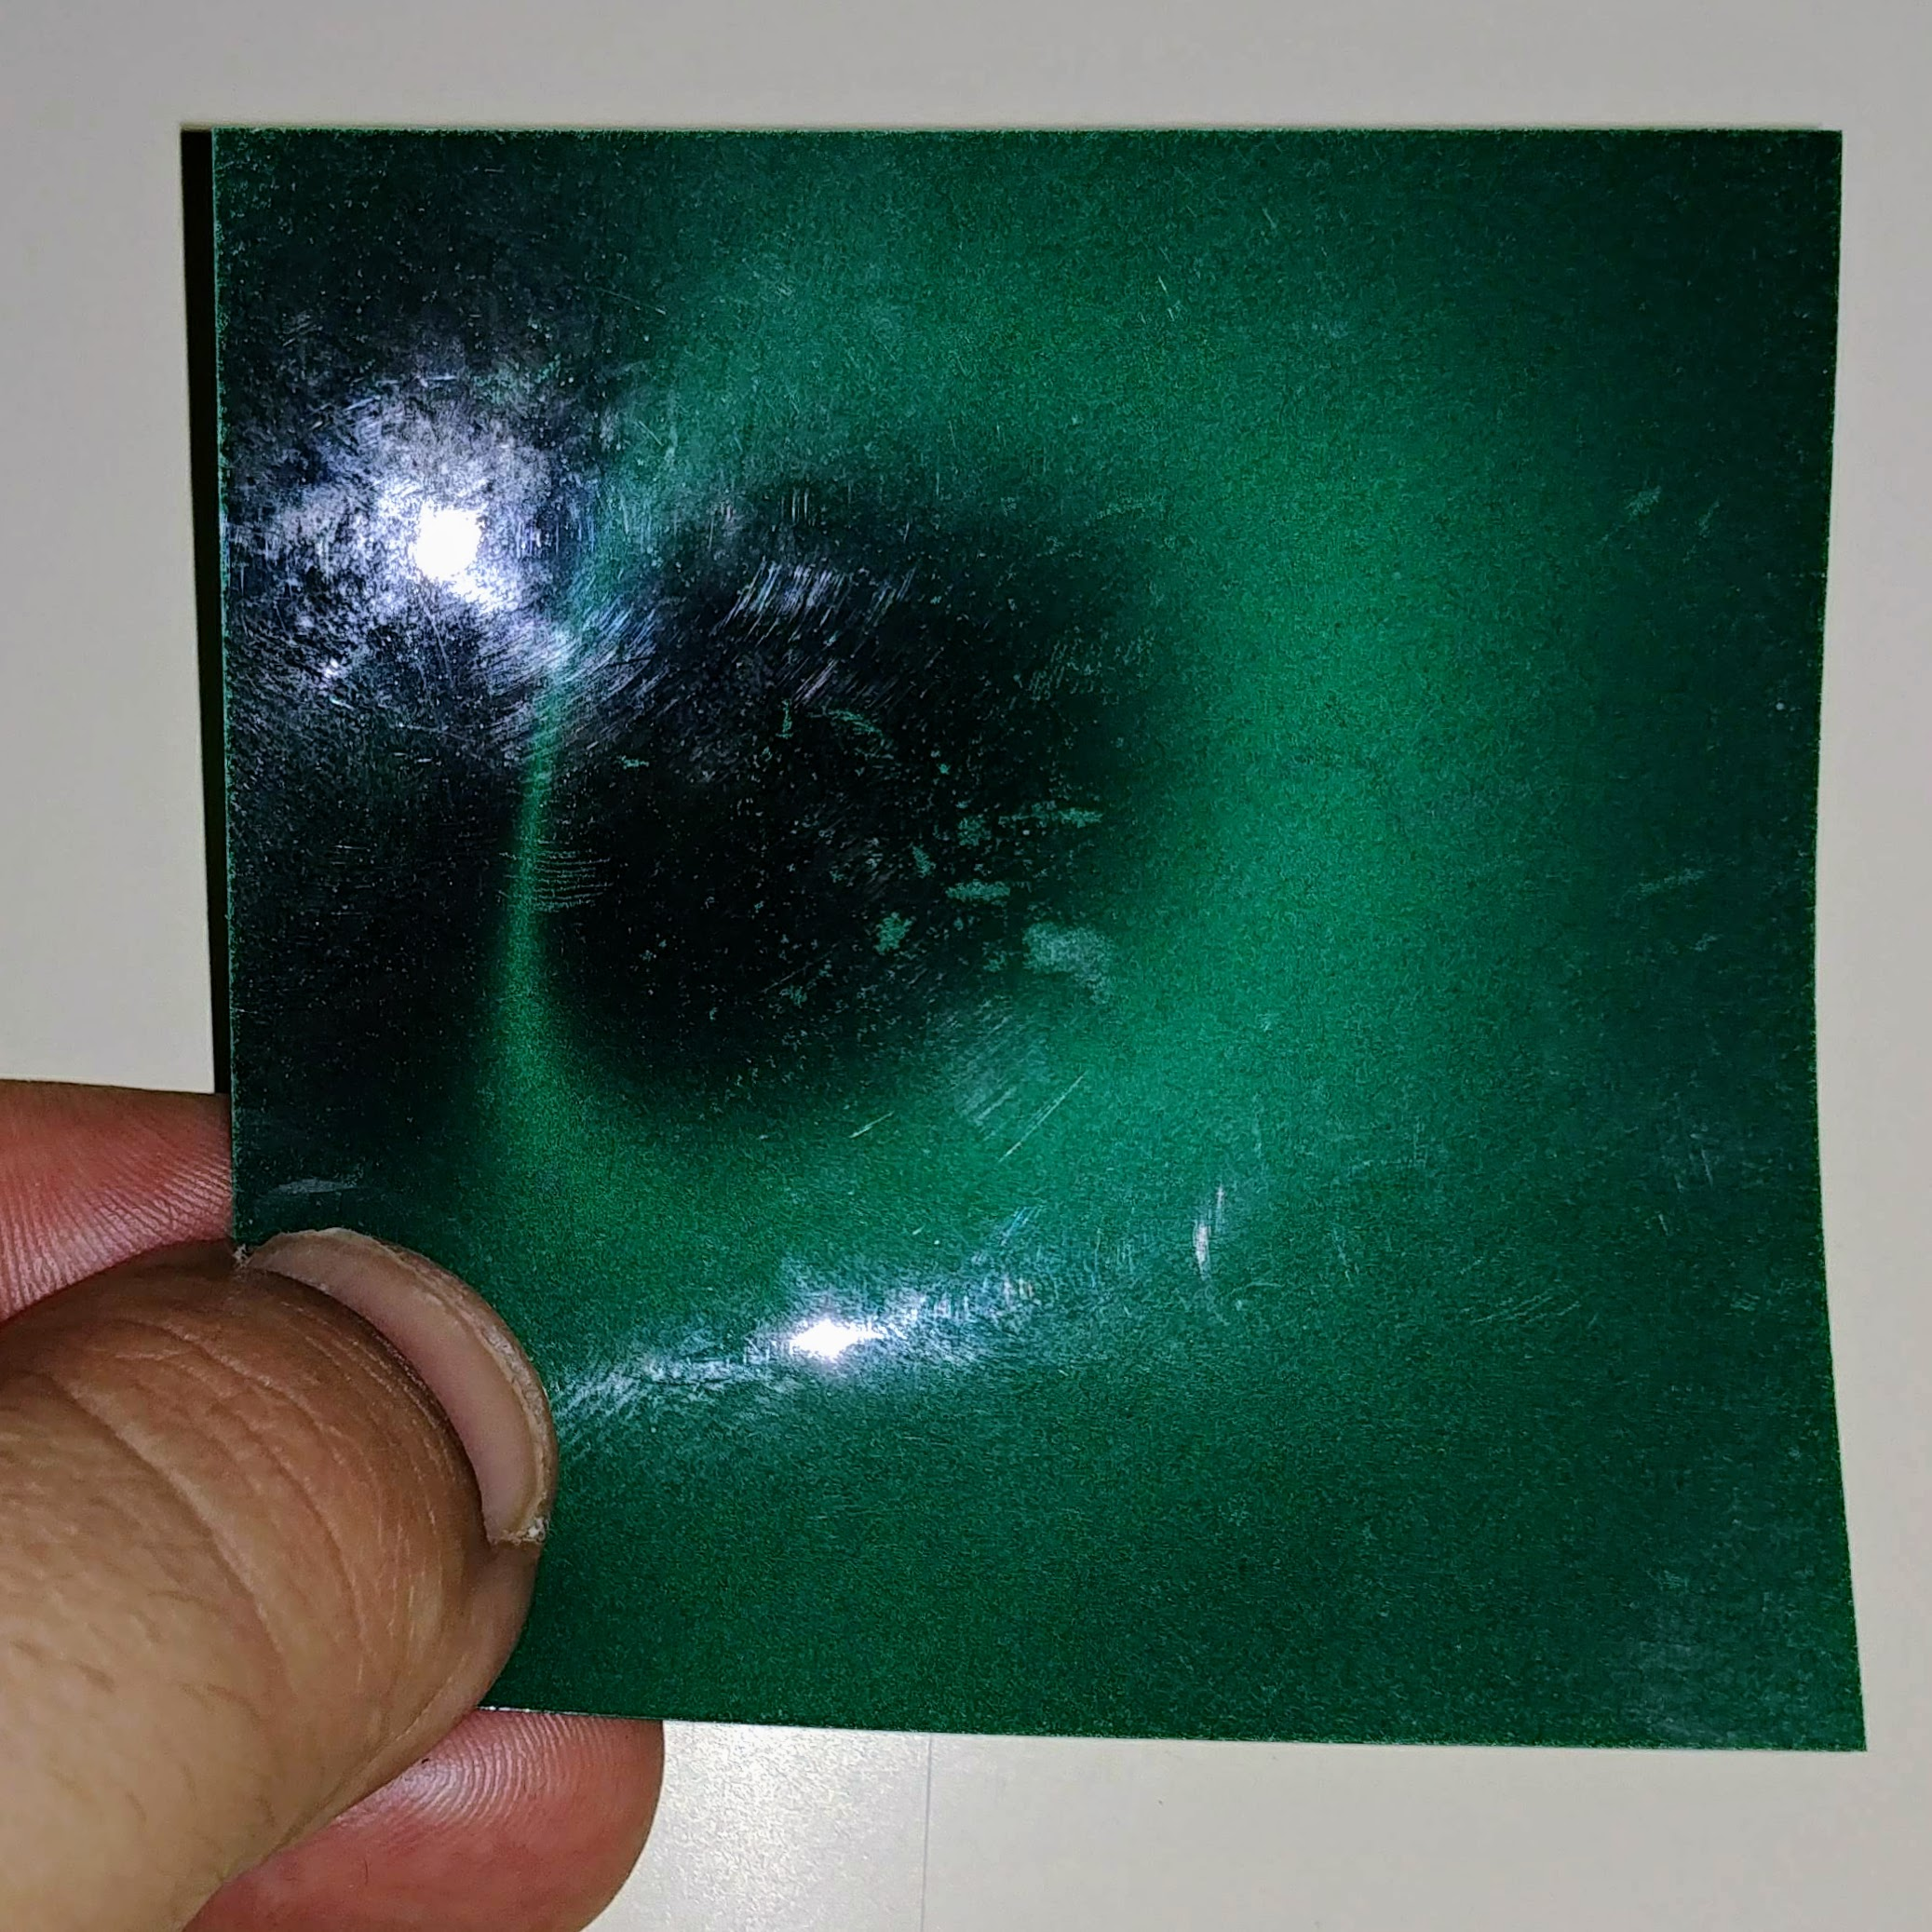
\includegraphics[width=.3\linewidth]{fig/experimentos/visualizacion_B_2}
	}
	\caption{Campos magnéticos de un imán de neodimio esférico}
\end{figure}
\end{frame}

\section{El motor eléctrico más sencillo del mundo}
\subsection{Introducción teórica}
\begin{frame}{Fuerza magnética sobre una corriente}
\begin{block}{Fuerza magnética sobre una corriente}
Una corriente $I$, con una longitud $L$, situado en un campo magnético $\magnFlux$, experimenta una fuerza:
$$
\vec{F}_m = \int_L I d\vec{l} \times \magnFlux
$$
\end{block}
La fuerza total sobre ese conductor se puede expresar como $F=I l B_\perp$ o, en forma vectorial, como
$$
\vec{F} = I \vec{l} \times \vec{B}
$$
\end{frame}

\begin{frame}{Fuerza sobre una espira}
\begin{block}{Momento dipolar magnético}
	\justifying
	El análogo magnético del momento dipolar eléctrico es el \textbf{momento magnético} que se puede expresar como,
	$$ \vec{\mu} = I A \hat{n} 	$$
	Donde $I$ es la corriente que circula por una espira de área $A$. El vector $\hat{n}$ es normal a la superficie con una orientación indicada por el sentido de la corriente siguiendo la regla de la mano derecha. 
\end{block}
\begin{block}{Torque en una espira}
La fuerza neta sobre un lazo de corriente en un campo magnético \textbf{uniforme} es cero. Sin embargo, el torque se puede expresar como,
$$ \vec{\tau} = \vec{\mu} \times \magnFlux $$
\end{block}
\end{frame}

\begin{frame}{Ejemplos: Motor de corriente continua y homopolar}
\begin{figure}
	\centering
	\subfloat[Motor DC. \newline \newline \tiny Fuente: Wikipedia, CC BY-SA 3.0]{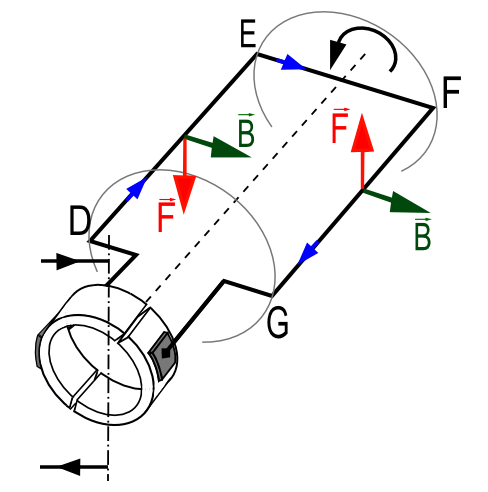
\includegraphics[width=.45\linewidth]{motor_dc}} \,
	\subfloat[Motor homopolar. \newline \newline \tiny Fuente: Wikipedia, dominio público]{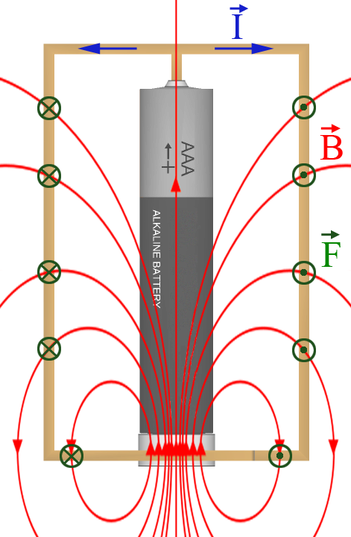
\includegraphics[width=.3\linewidth]{fig/motor_homopolar}}
	\caption{Distintos tipos de motores eléctricos.}
\end{figure}
\end{frame}

\subsection{Diseño experimental}
\begin{frame}{Materiales}
\begin{figure}
\centering
\subfloat[Latas de acero (izda.) y aluminio (dcha.)]{
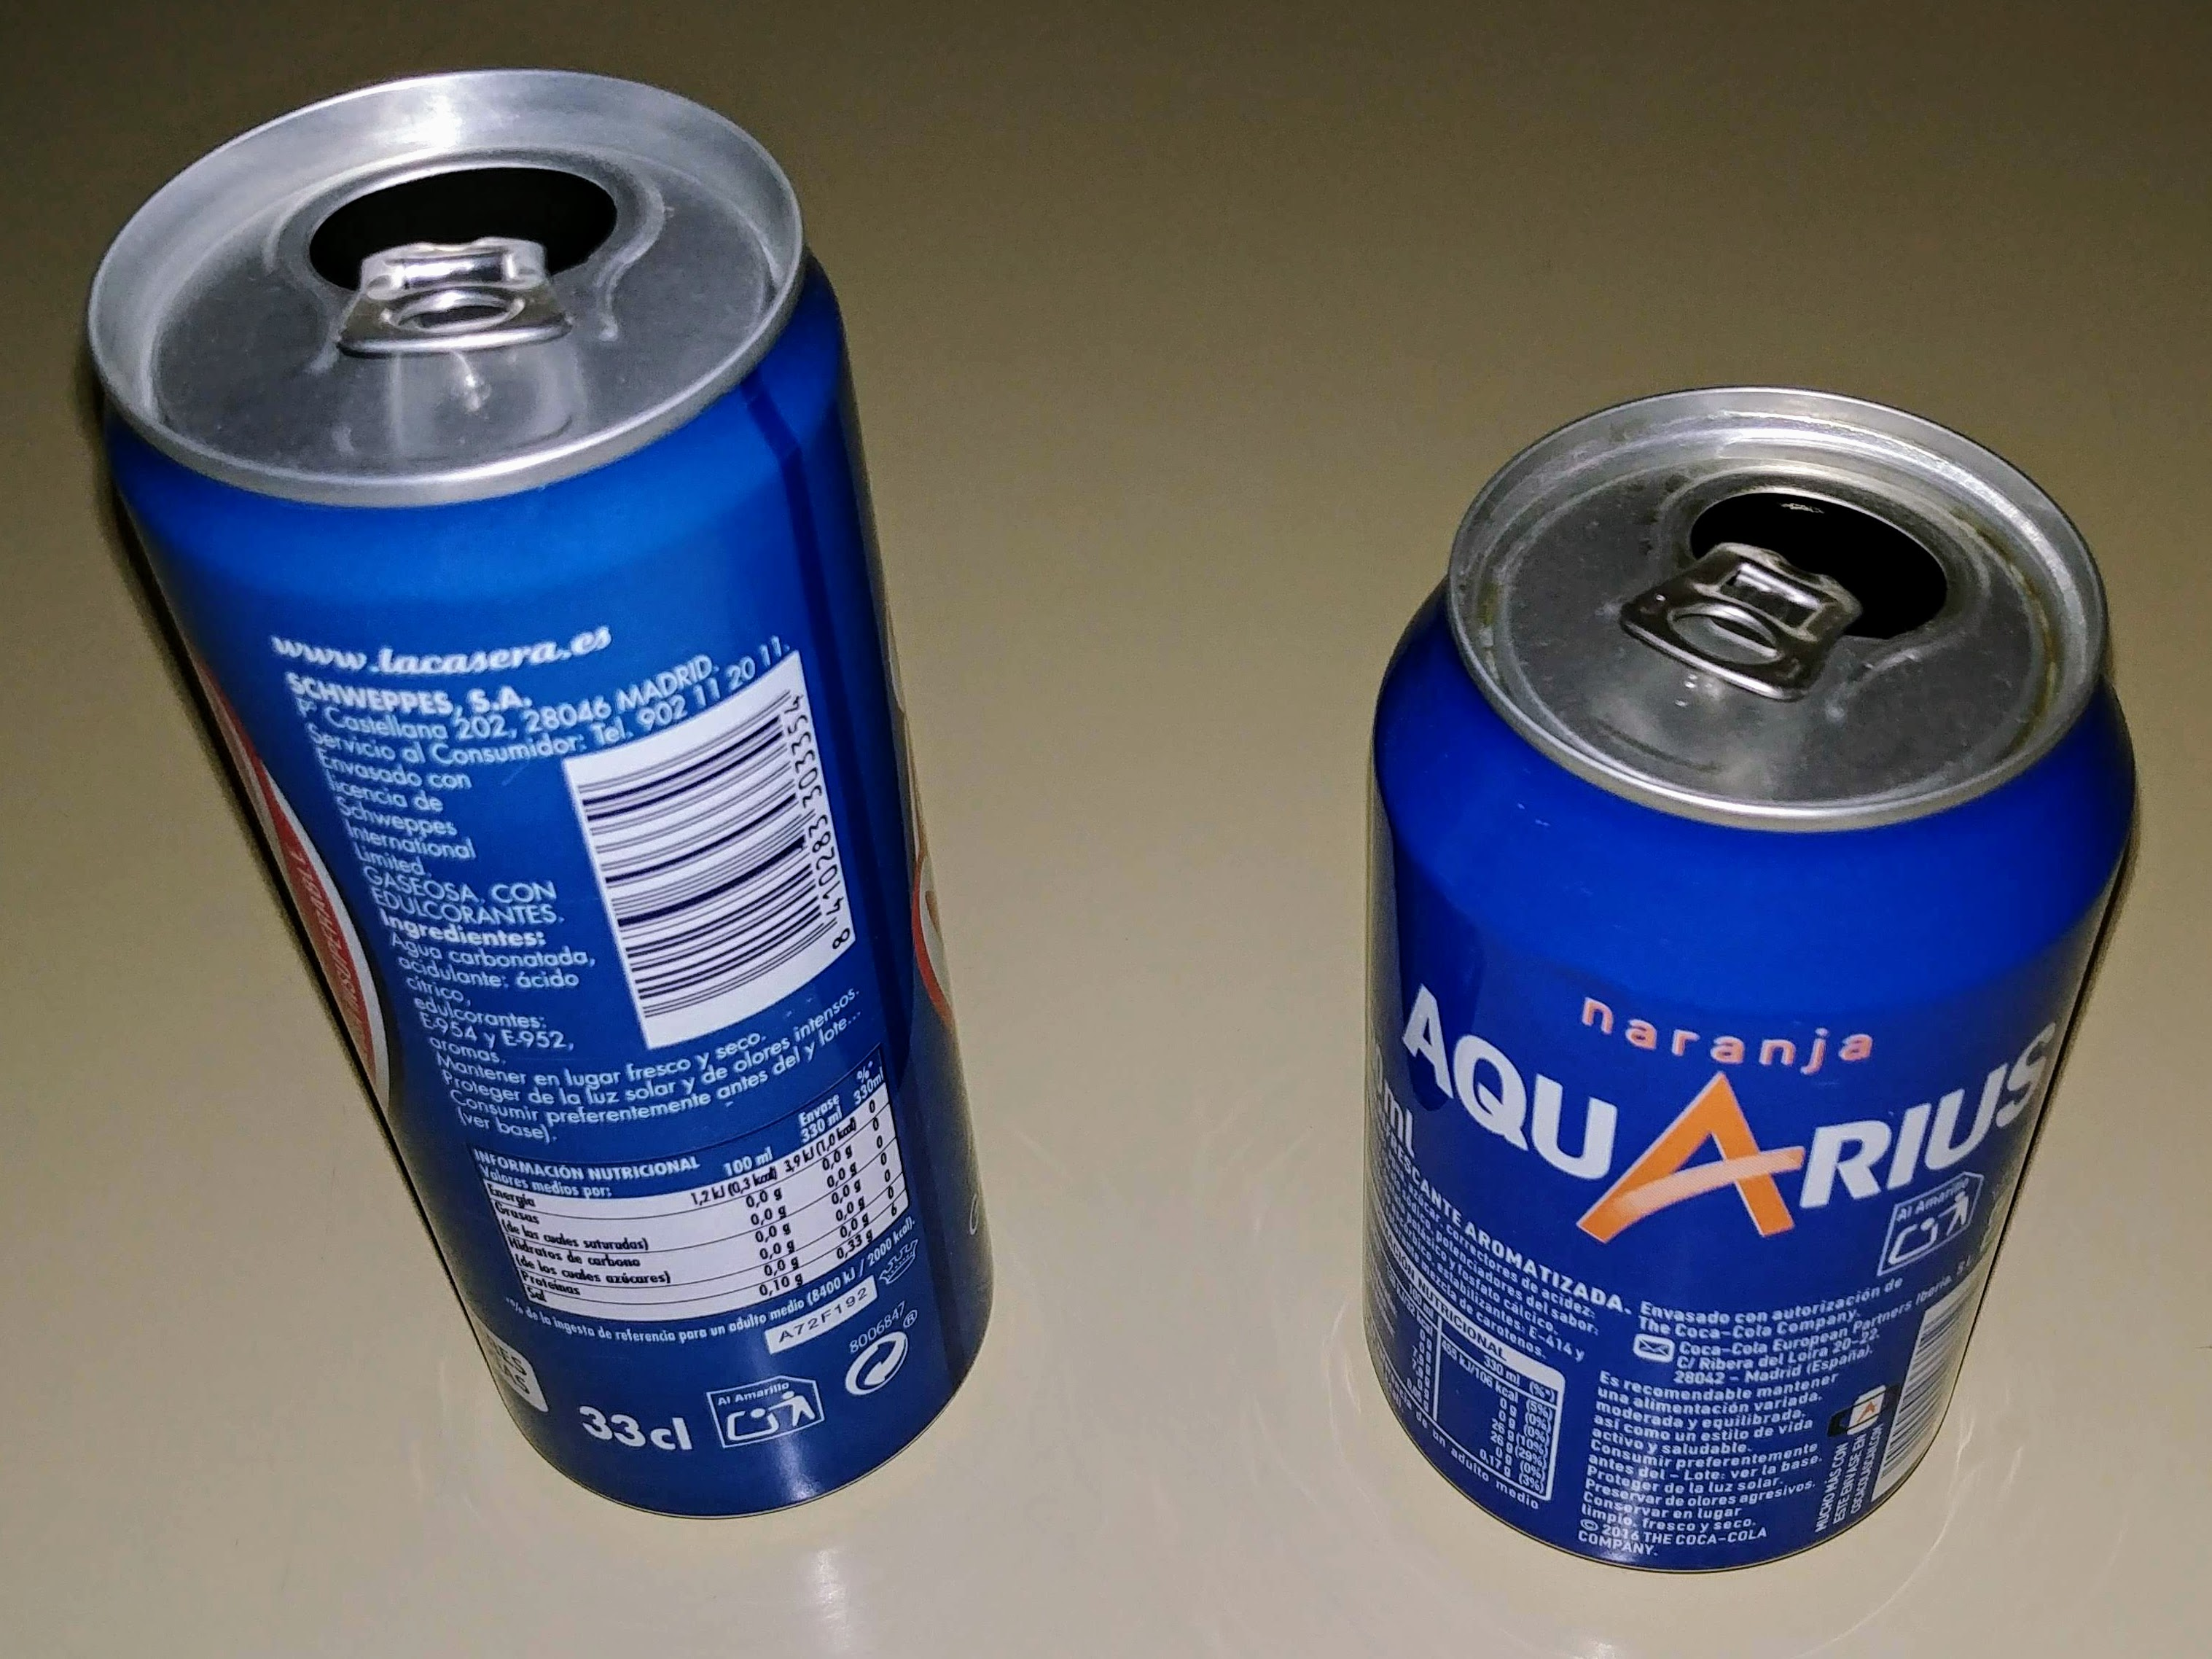
\includegraphics[width=.4\linewidth]{fig/experimentos/latas}
}\,
\subfloat[Hilo de cobre, pila, e imán en forma de disco (bajo la pila)]{
	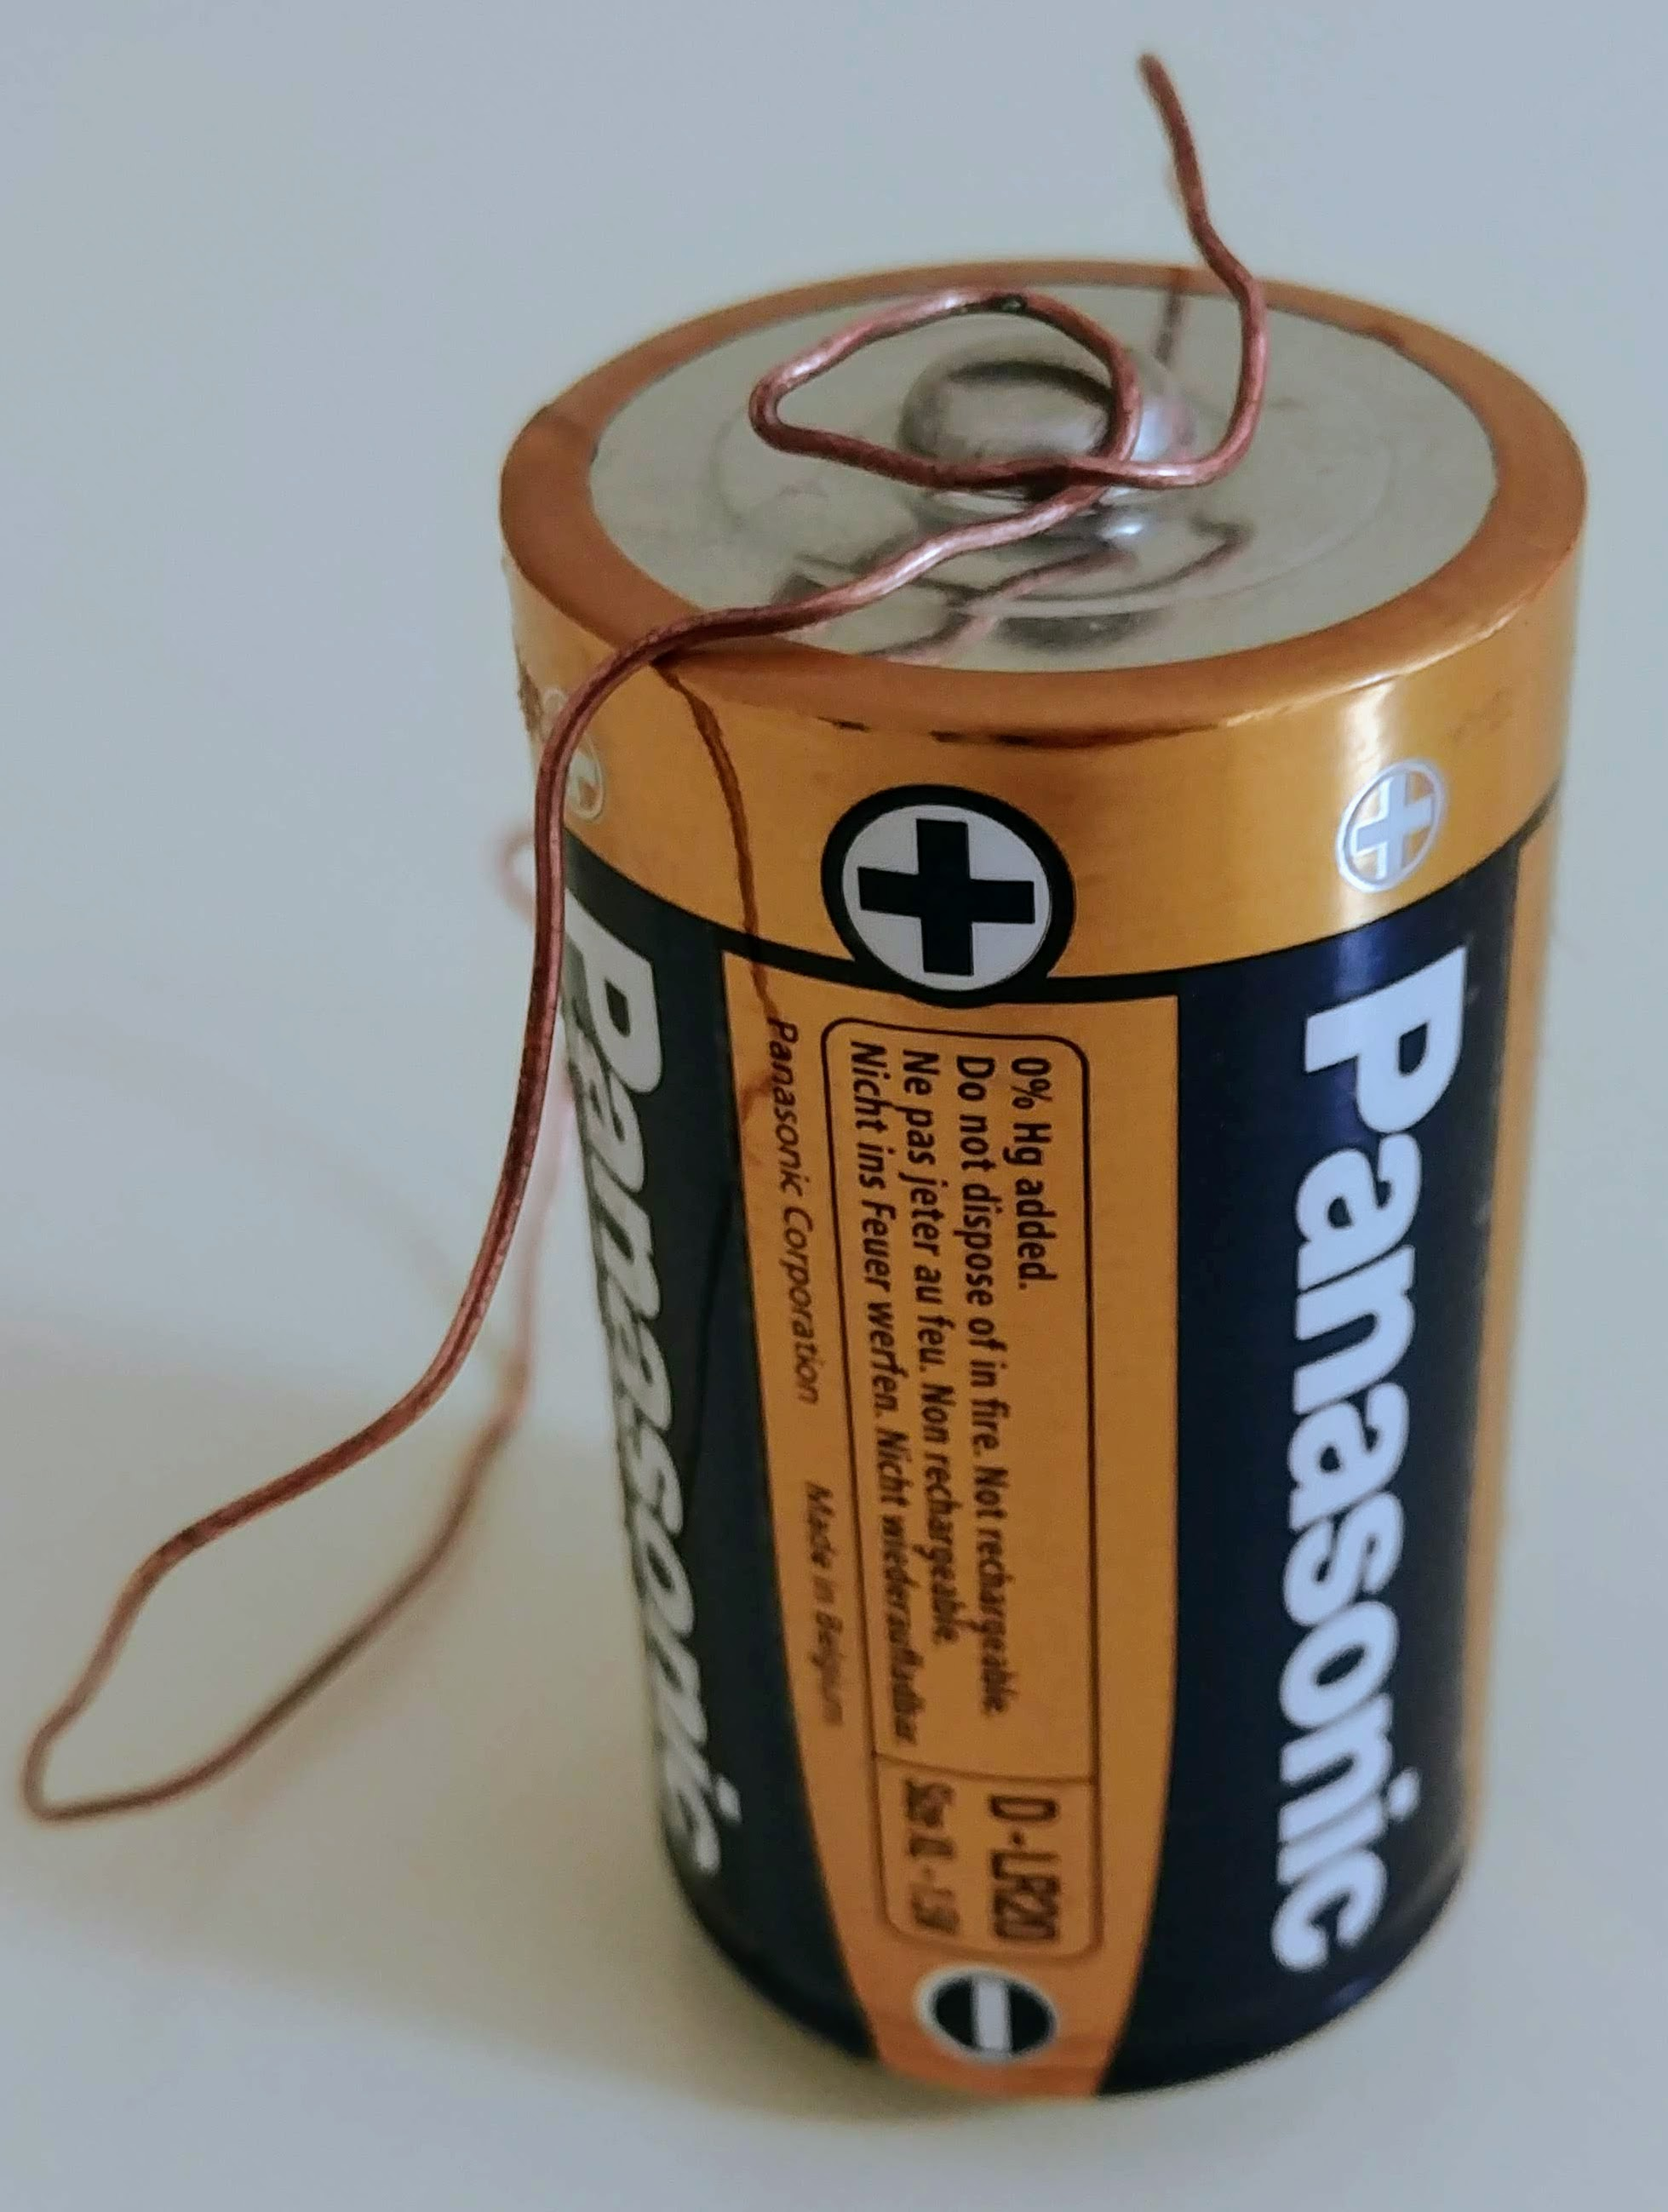
\includegraphics[width=.25\linewidth]{fig/experimentos/motor_dc}
}\,
\subfloat[Motor homopolar empleando un tornillo, hilo de cobre, una pila, imanes en forma de disco, y papel de aluminio]{
	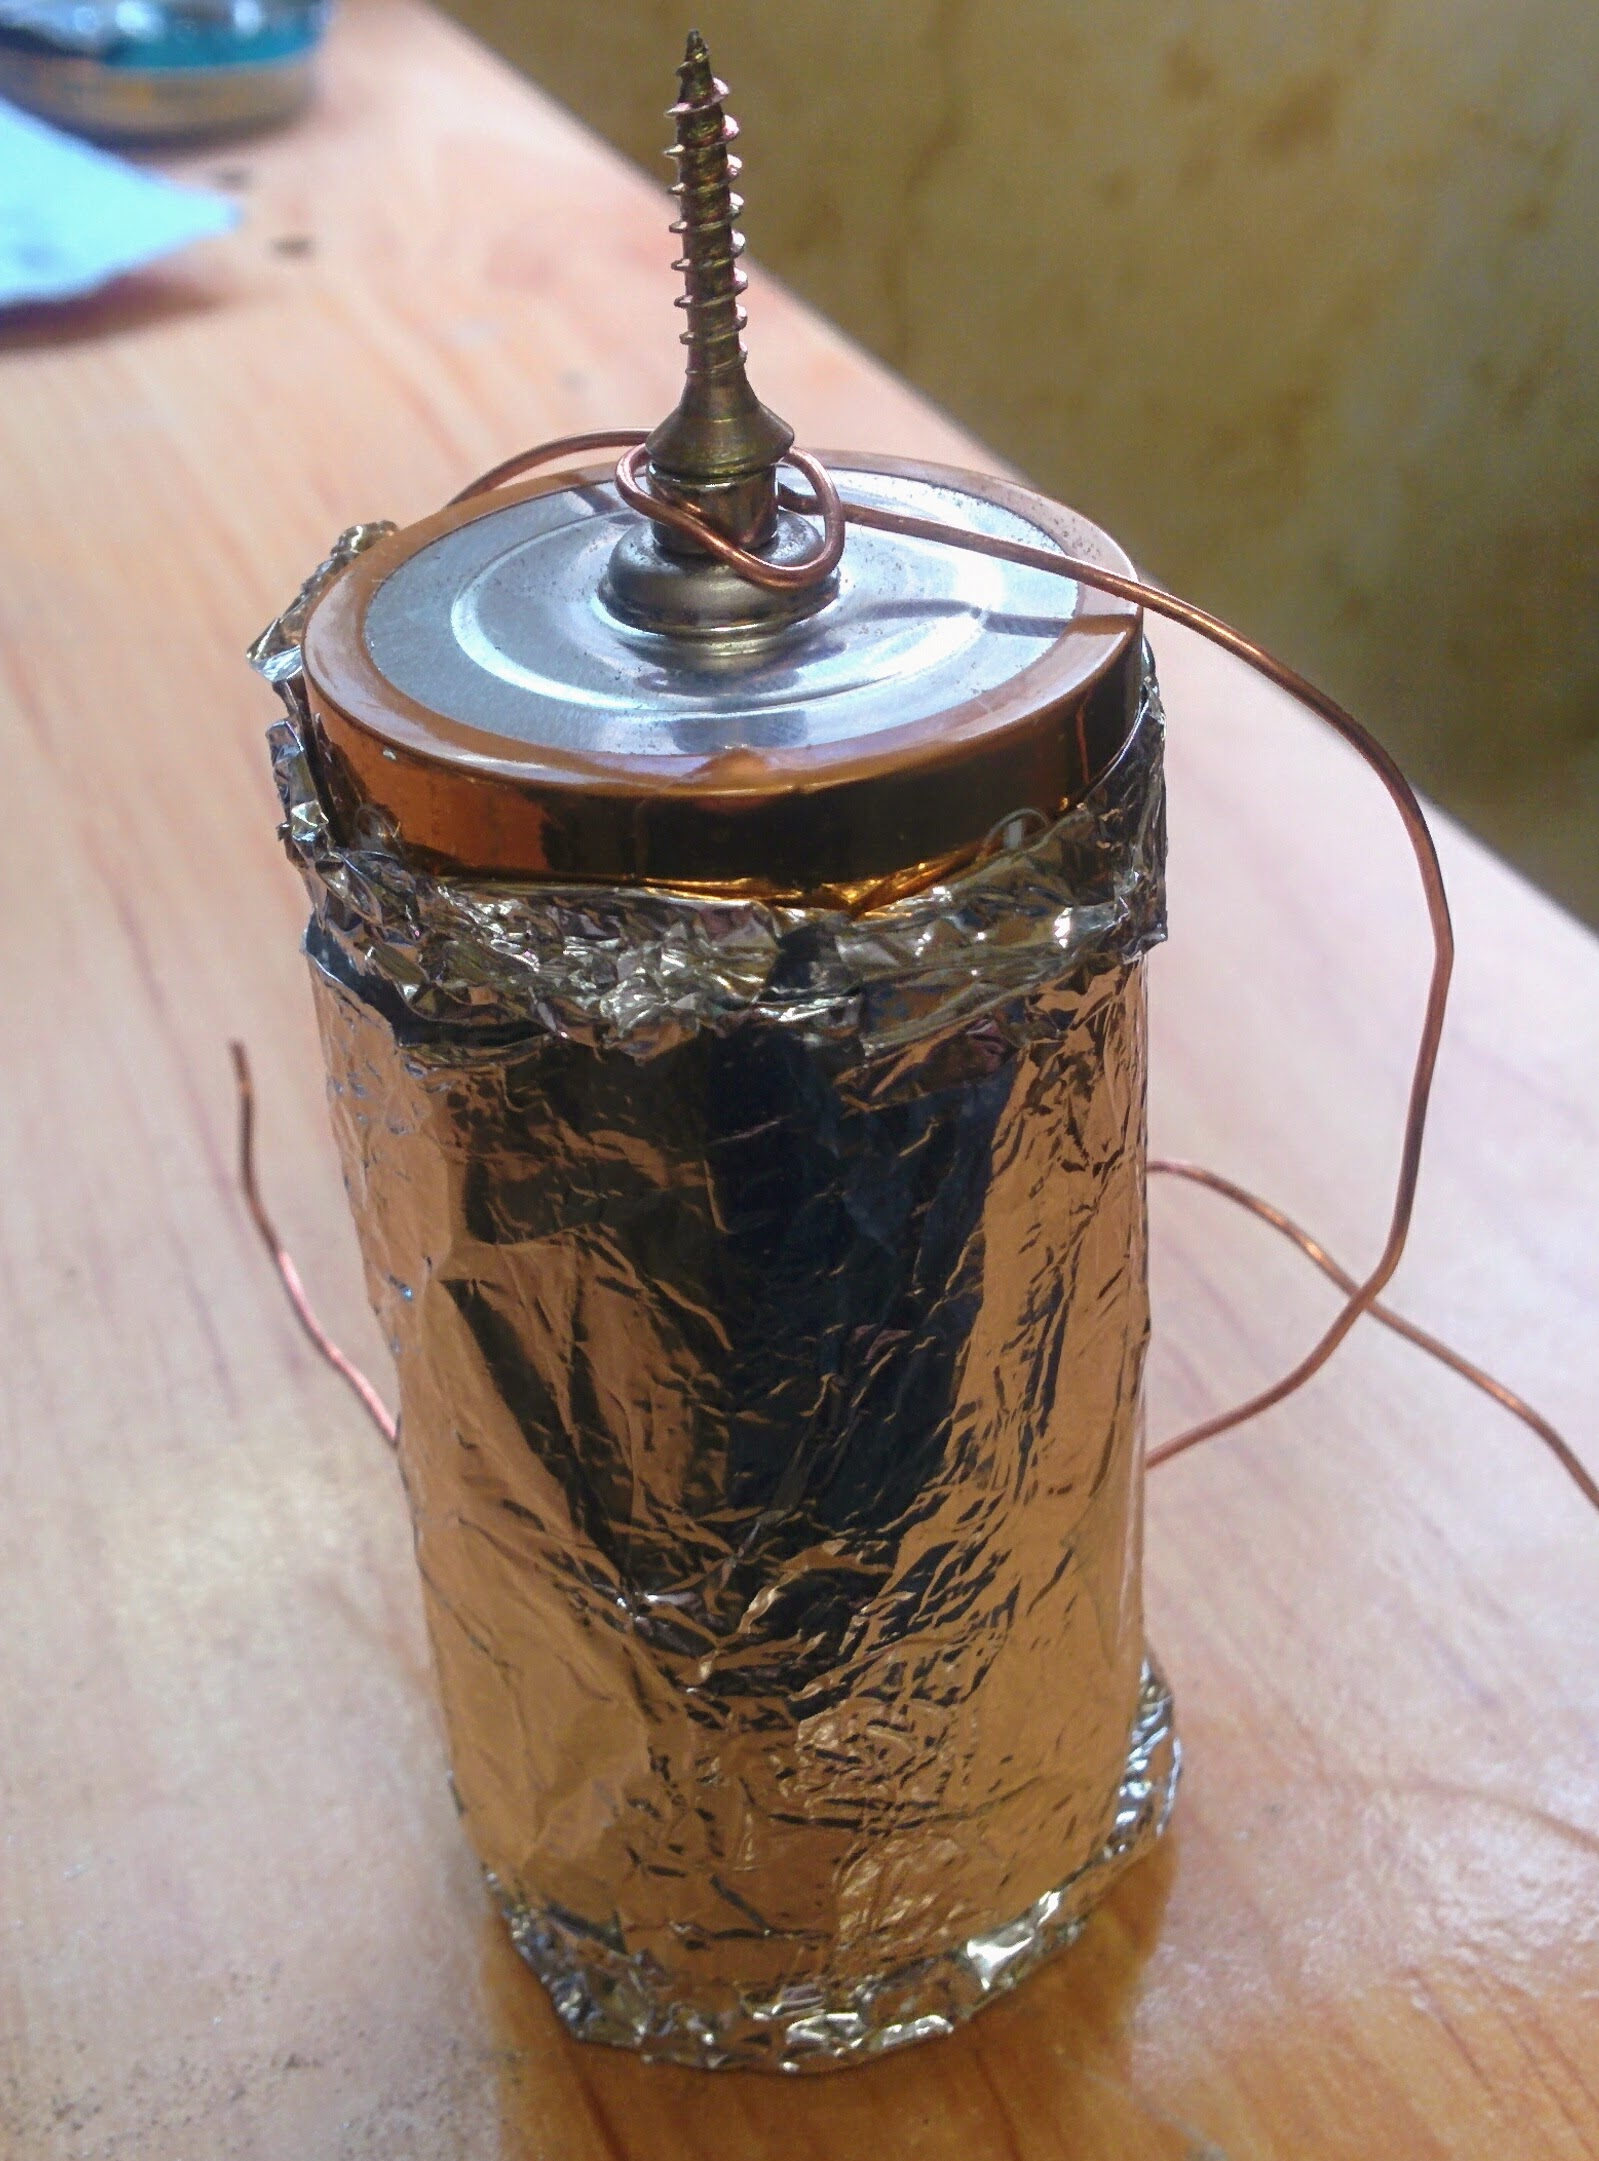
\includegraphics[width=.25\linewidth]{fig/experimentos/motor_pila_aluminio}
}\,
\end{figure}
\end{frame}

\begin{frame}{Ejemplos}
\begin{figure}
	\centering
	\subfloat[Motor hecho con una pila, imanes e hilo de cobre]{			    
		\movie[]{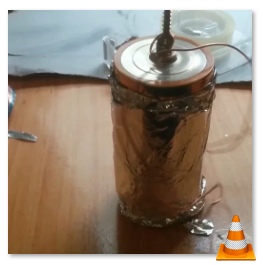
\includegraphics[width=.4\linewidth]{fig/experimentos/motor_pila}}{fig/experimentos/motor_pila.avi}
	}
	\subfloat[Motor hecho con una pila, imanes y lata] {
		\movie[]{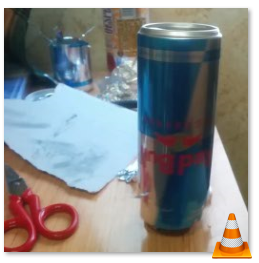
\includegraphics[width=.4\linewidth]{fig/experimentos/motor_lata}}{fig/experimentos/motor_lata.avi}
	}
\end{figure}
\end{frame}

\section{Fuerzas sobre corrientes}
\subsection{Introducción teórica}
\begin{frame}{Ley de Inducción de Faraday}
	\begin{block}{Ley de inducción de Faraday en un lazo cerrado}
		La FEM inducida en un lazo cerrado es igual al negativo de la tasa de cambio del flujo magnético a través del lazo.
		$$
		\emf = - \frac{d\Phi_B}{dt} \ \ \ [\Volt]
		$$
	\end{block}
\end{frame}

\begin{frame}
	\begin{block}{Ley de inducción de Faraday}
		La ley de inducción de Faraday en forma integral es,
		$$
			\oint \elec \cdot d\vec{l} = - \frac{d\Phi_B}{dt}
		$$
	\end{block}	
    \begin{block}{Ley de Lenz}
		La polaridad de una corriente inducida es tal que el campo magnético que esta genera tiende a oponerse al campo que las genera.
	\end{block}
\end{frame}

\begin{frame}{Corrientes de Foucault}
\begin{figure}
	\centering
	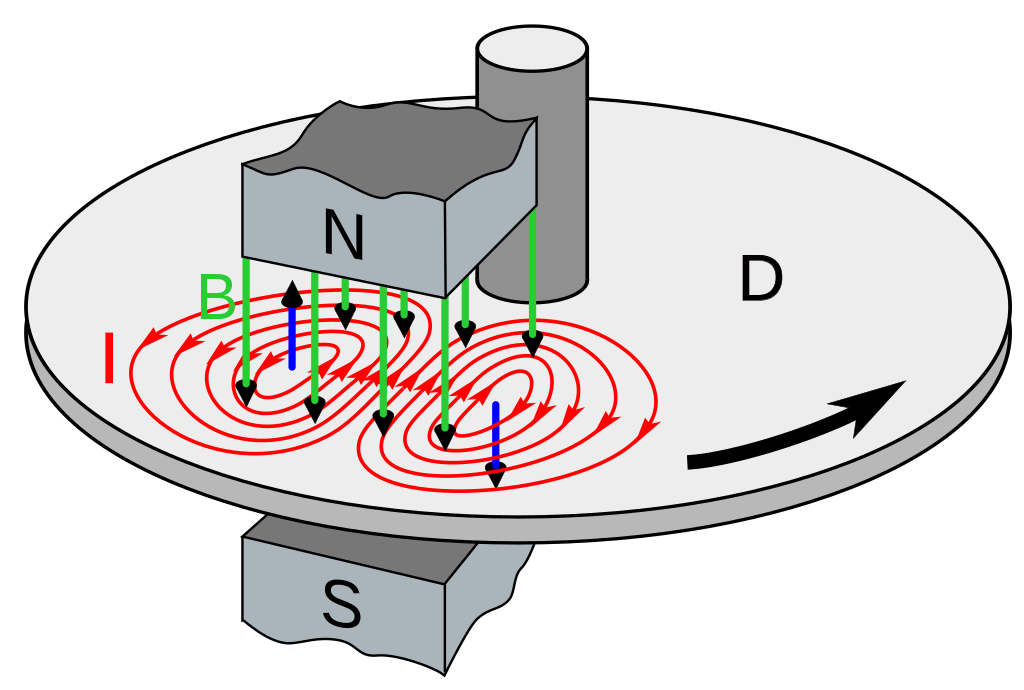
\includegraphics[width=0.7\linewidth]{eddy_current.png}
\end{figure}
\end{frame}

\begin{frame}
\begin{columns}
	\column{0.5\textwidth}  
	\begin{figure}
		\centering
		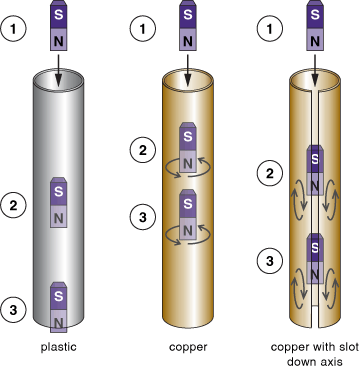
\includegraphics[width=1\linewidth]{ind_lenz_08_co.png}
		\caption{\tiny Fuente: NSW, Department of Education of Australia.}
	\end{figure}
	\column{0.5\textwidth}  
	\begin{enumerate}
		\item Al soltar un iman dentro de un tubo de cobre se producen unas corrientes de Foucault debido a su movimiento.
		\item Estas corrientes generan a su vez un campo magnético con la polaridad contraria a la del imán.
		\item Los campos magnéticos inducidos frenan la caida del imán.
	\end{enumerate}
\end{columns}
\end{frame}

\subsection{Diseño experimental}
\begin{frame}{Materiales}
\begin{figure}
	\centering
	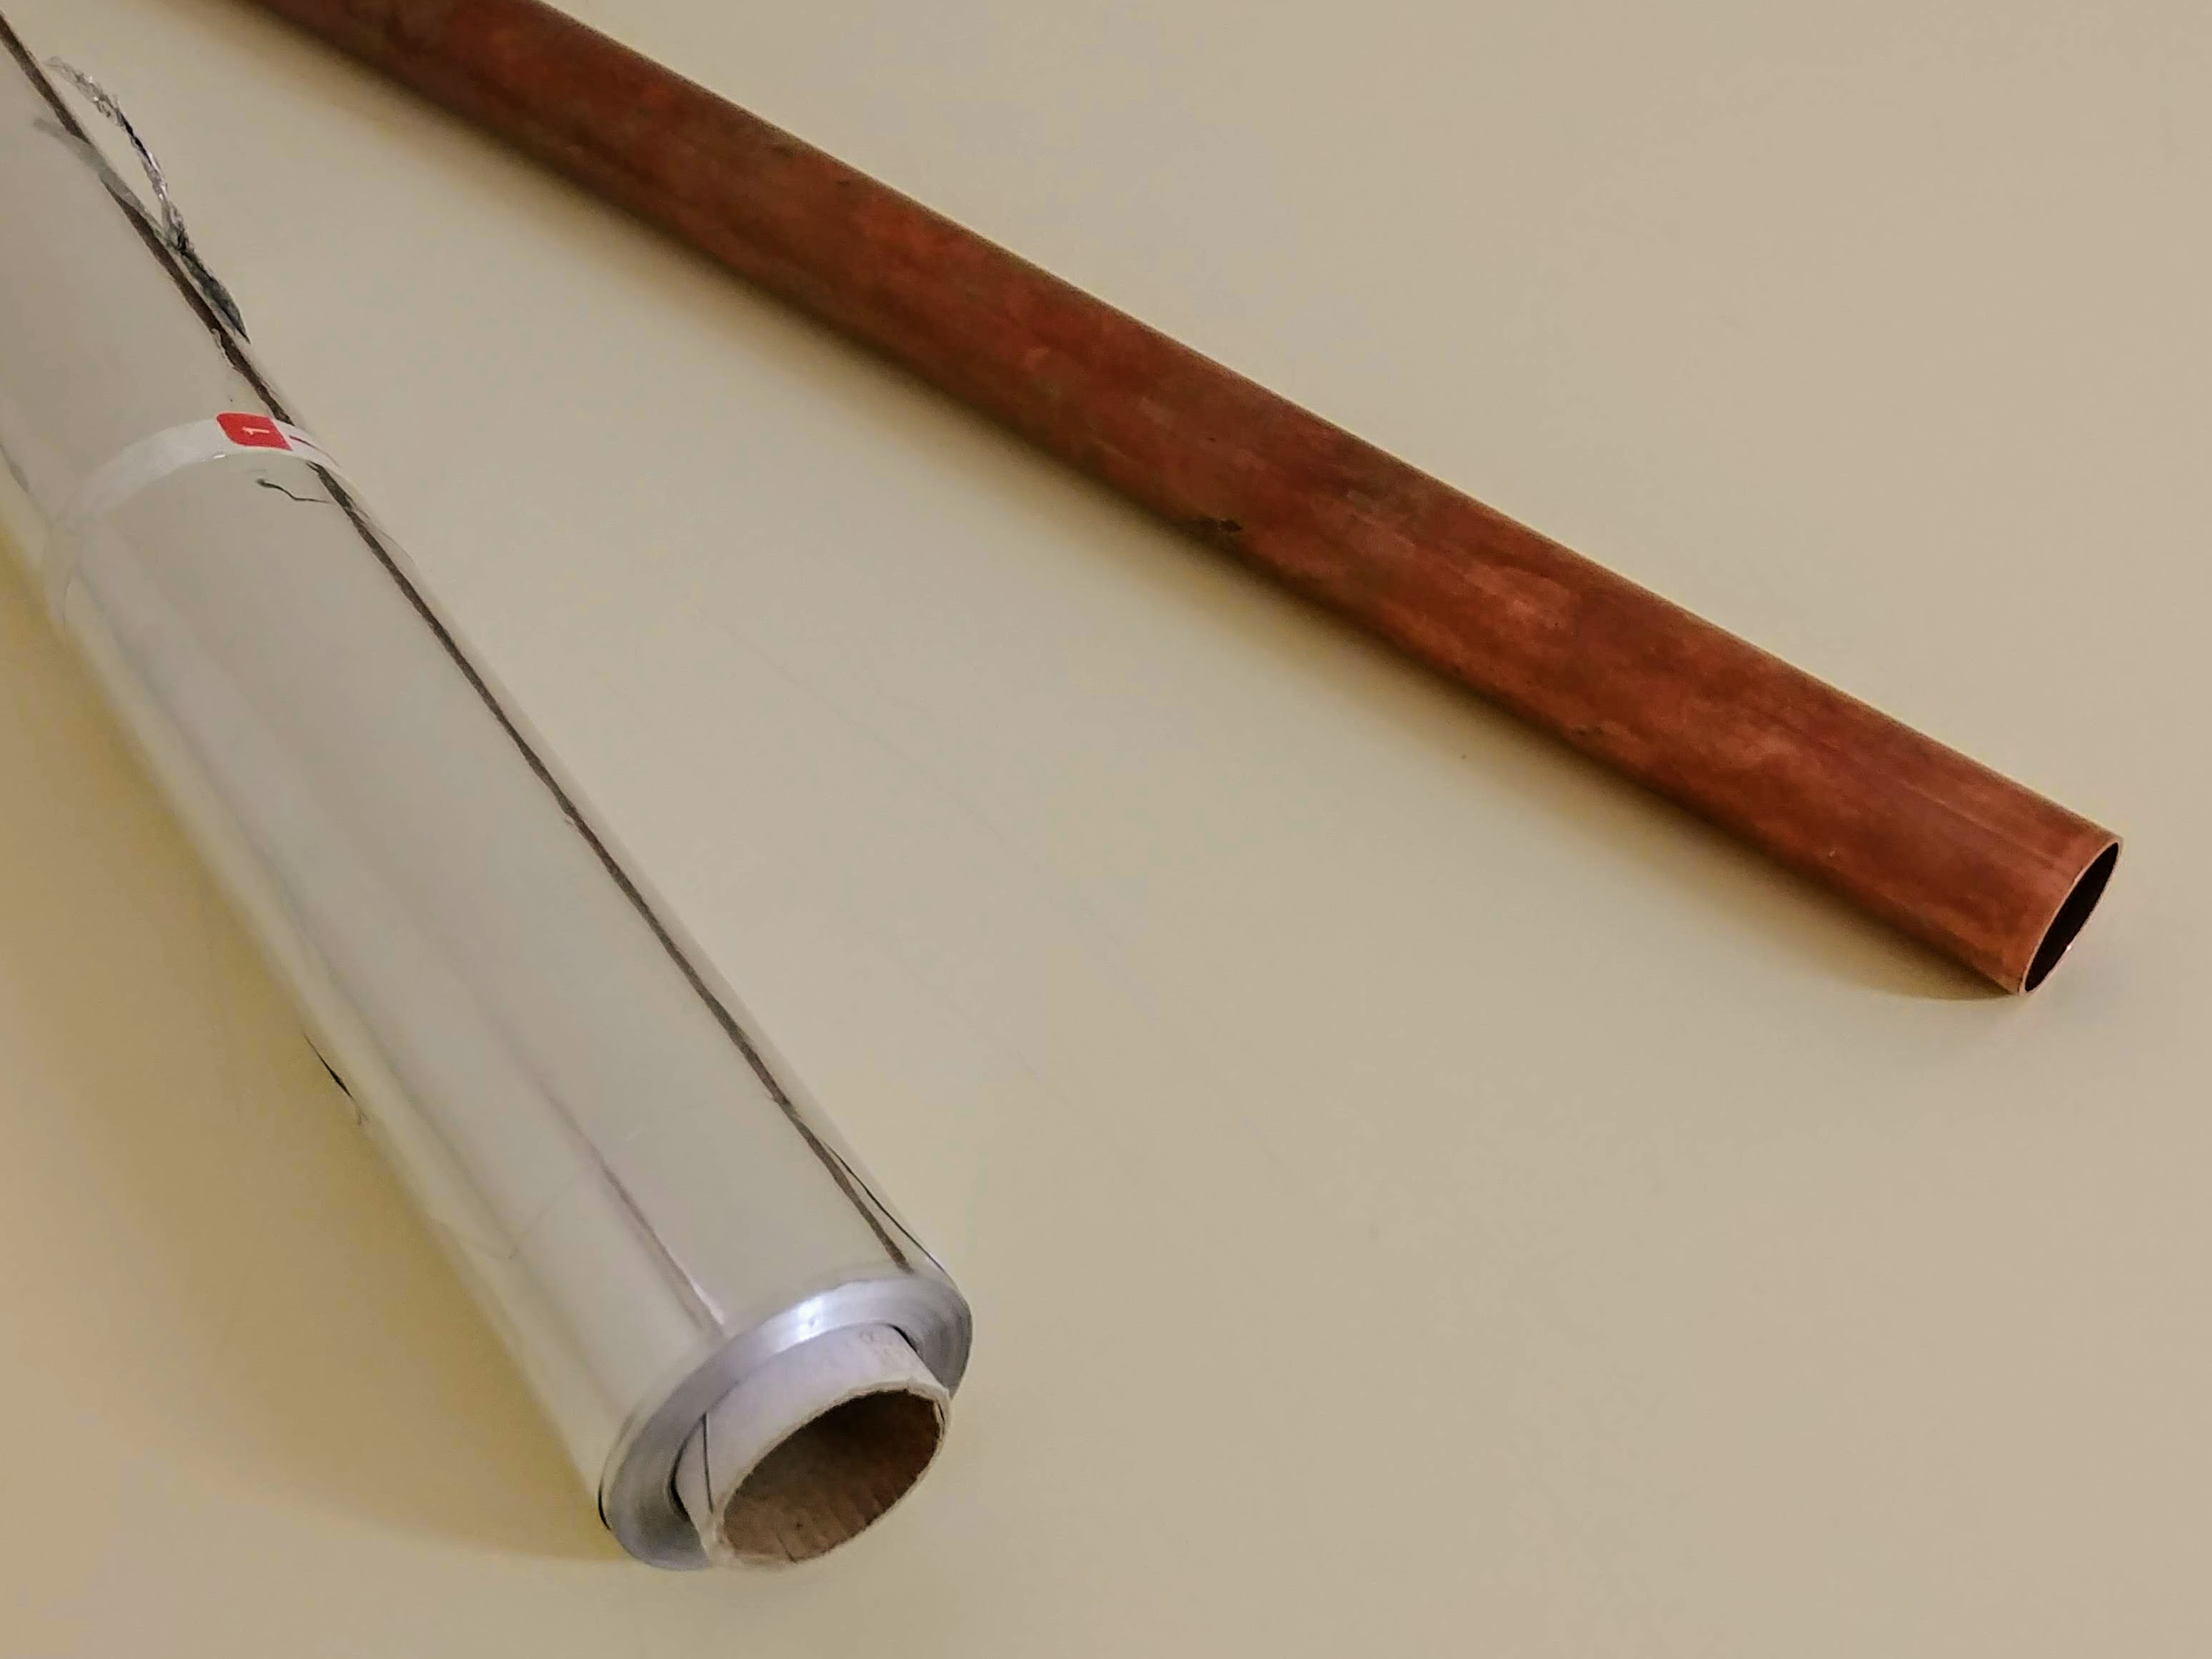
\includegraphics[width=.6\linewidth]{fig/experimentos/tubo_cobre_y_aluminio}
	\caption{\justifying Un imán de neodimio esférico es ralentizado a medida que cae por tubos tantos de aluminio (izda.) como de cobre (dcha.). En reposo, estos materiales son paramagnéticos y no se ven apenas afectados por imanes. La única explicación son las corrientes inducidas en ellos.}
\end{figure}
\end{frame}

\section{Materiales diamagnéticos, paramagnéticos, y ferromagnéticos}
\subsection{Introducción teórica}
\begin{frame}{Materiales magnéticos}
	\justifying
	Los átomos tienen una corteza electrónica en movimiento cuyos electrones forman lazos microscópicos de corriente que producen campos magnéticos por si mismos, es decir que poseen un \textbf{momento dipolar magnético}, $\vec{\mu}$.
	\begin{itemize}
		\item Si estos están orientados al azar, en suma el campo magnético será cero.
		\item Si están alineados, generaran un campo magnético y entonces diremos que el material está \textbf{magnetizado}.
	\end{itemize}
	La magnetización $\vec{M}$ se puede expresar, como la suma de todos los momentos magnéticos por una unidad de volumen:
	$
	\vec{M} = \frac{\sum{\vec{\mu}}}{V}
	$
	
	Y el campo magnético efectivo como:
	$$
	\vec{B}_\text{efectivo} = \vec{B} + \mu_0 \vec{M}
	$$

\end{frame}

\begin{frame}{Clasificación}
	\begin{itemize}
		\justifying
		\item Los materiales \textbf{paramagnéticos} responden magnetizándose parcialmente \textbf{mientras} se encuentran en presencia de un campo magnético \textbf{en la dirección del mismo}. Esto se traduce en que tienen una permeabilidad magnética efectiva \textbf{mayor} que la del vacío: $\permeability = K_M \permeability_0 = \permeability_r \permeability_0 $, con $K_M > 1$.
		\item Los materiales \textbf{diamagnéticos} responden \textbf{oponiéndose} al campo magnético debido al movimiento de su corteza electrónica. En consecuencia, su $K_M < 1$. Es decir, $\permeability$ \textbf{menor que} la del vacío.
		\item Los materiales \textbf{ferromagnéticos} tienen interacciones muy fuertes entre sus momentos magnéticos que dan lugar a dominios magnéticos. Quedan magnetizados incluso \textbf{sin presencia de campos magnéticos externos}. Por tanto tienen \textbf{histéresis}, es decir, que \textit{recuerdan} los campos magnéticos a los que han sido sometidos.
	\end{itemize}
\end{frame}

\begin{frame}{Ferromagnetismo y dependencia con la temperatura}
En los materiales ferromagnéticos existe una fuerte dependencia con la temperatura. 
\begin{itemize}
\item Por encima de una cierta temperatura, llamada temperatura de Curie, las interacciones térmicas dominan y los dipolos se orientan aleatoriamente.
\item Cuando $T$ baja, los dipolos tienden a alinearse con sus vecinos, dando lugar a los dominios magnéticos. Si al enfriarse existe un $\magnFlux$ externo, unos dominios predominarán sobre otros y el material se comportará como un imán permanente.
\end{itemize} 
Una simulación del fenómeno:
\begin{itemize}
\item  {\scriptsize \url{http://physics.weber.edu/schroeder/software/demos/IsingModel.html}}
\end{itemize}
Un video explicativo: {\scriptsize \url{https://www.youtube.com/watch?v=kjwKgpQ-l1s}}
\end{frame}

\subsection{Diseño experimental}
\begin{frame}{Materiales diamagnéticos}
\begin{figure}
	\centering
	\subfloat[Vista superior]{
		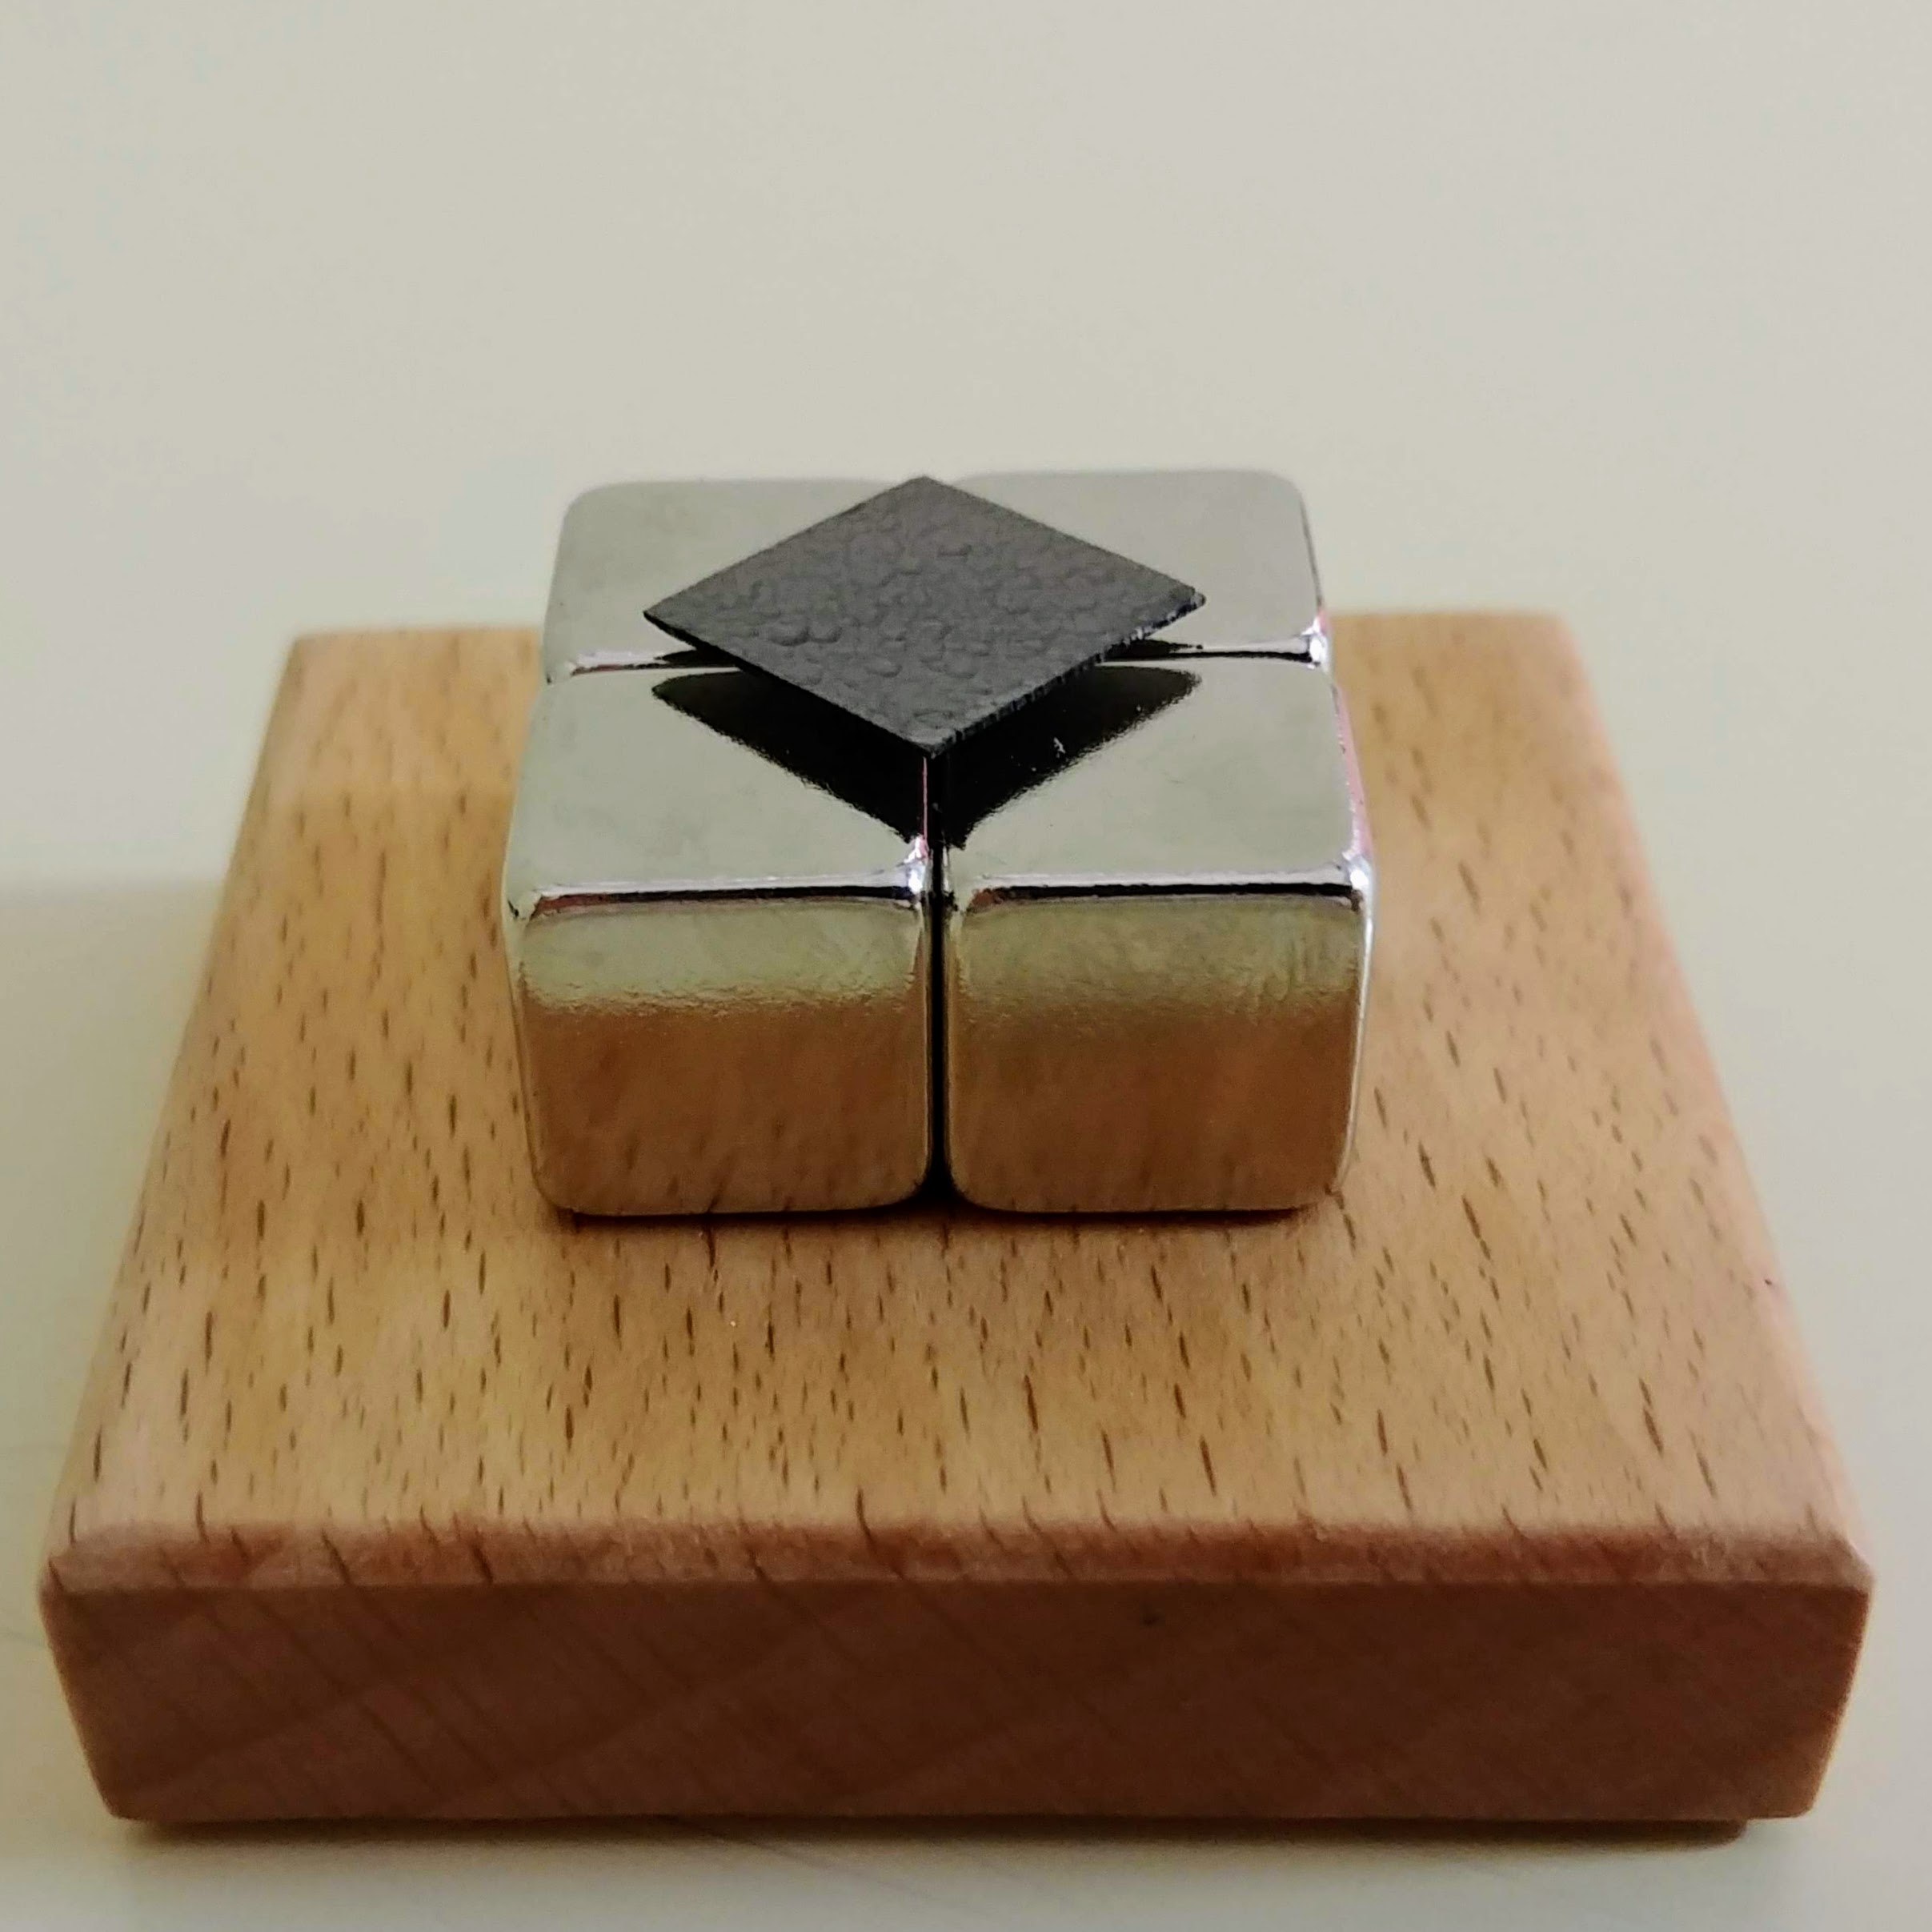
\includegraphics[width=.3\linewidth]{fig/experimentos/diamaglev_1}
	}\,
	\subfloat[Vista lateral]{
	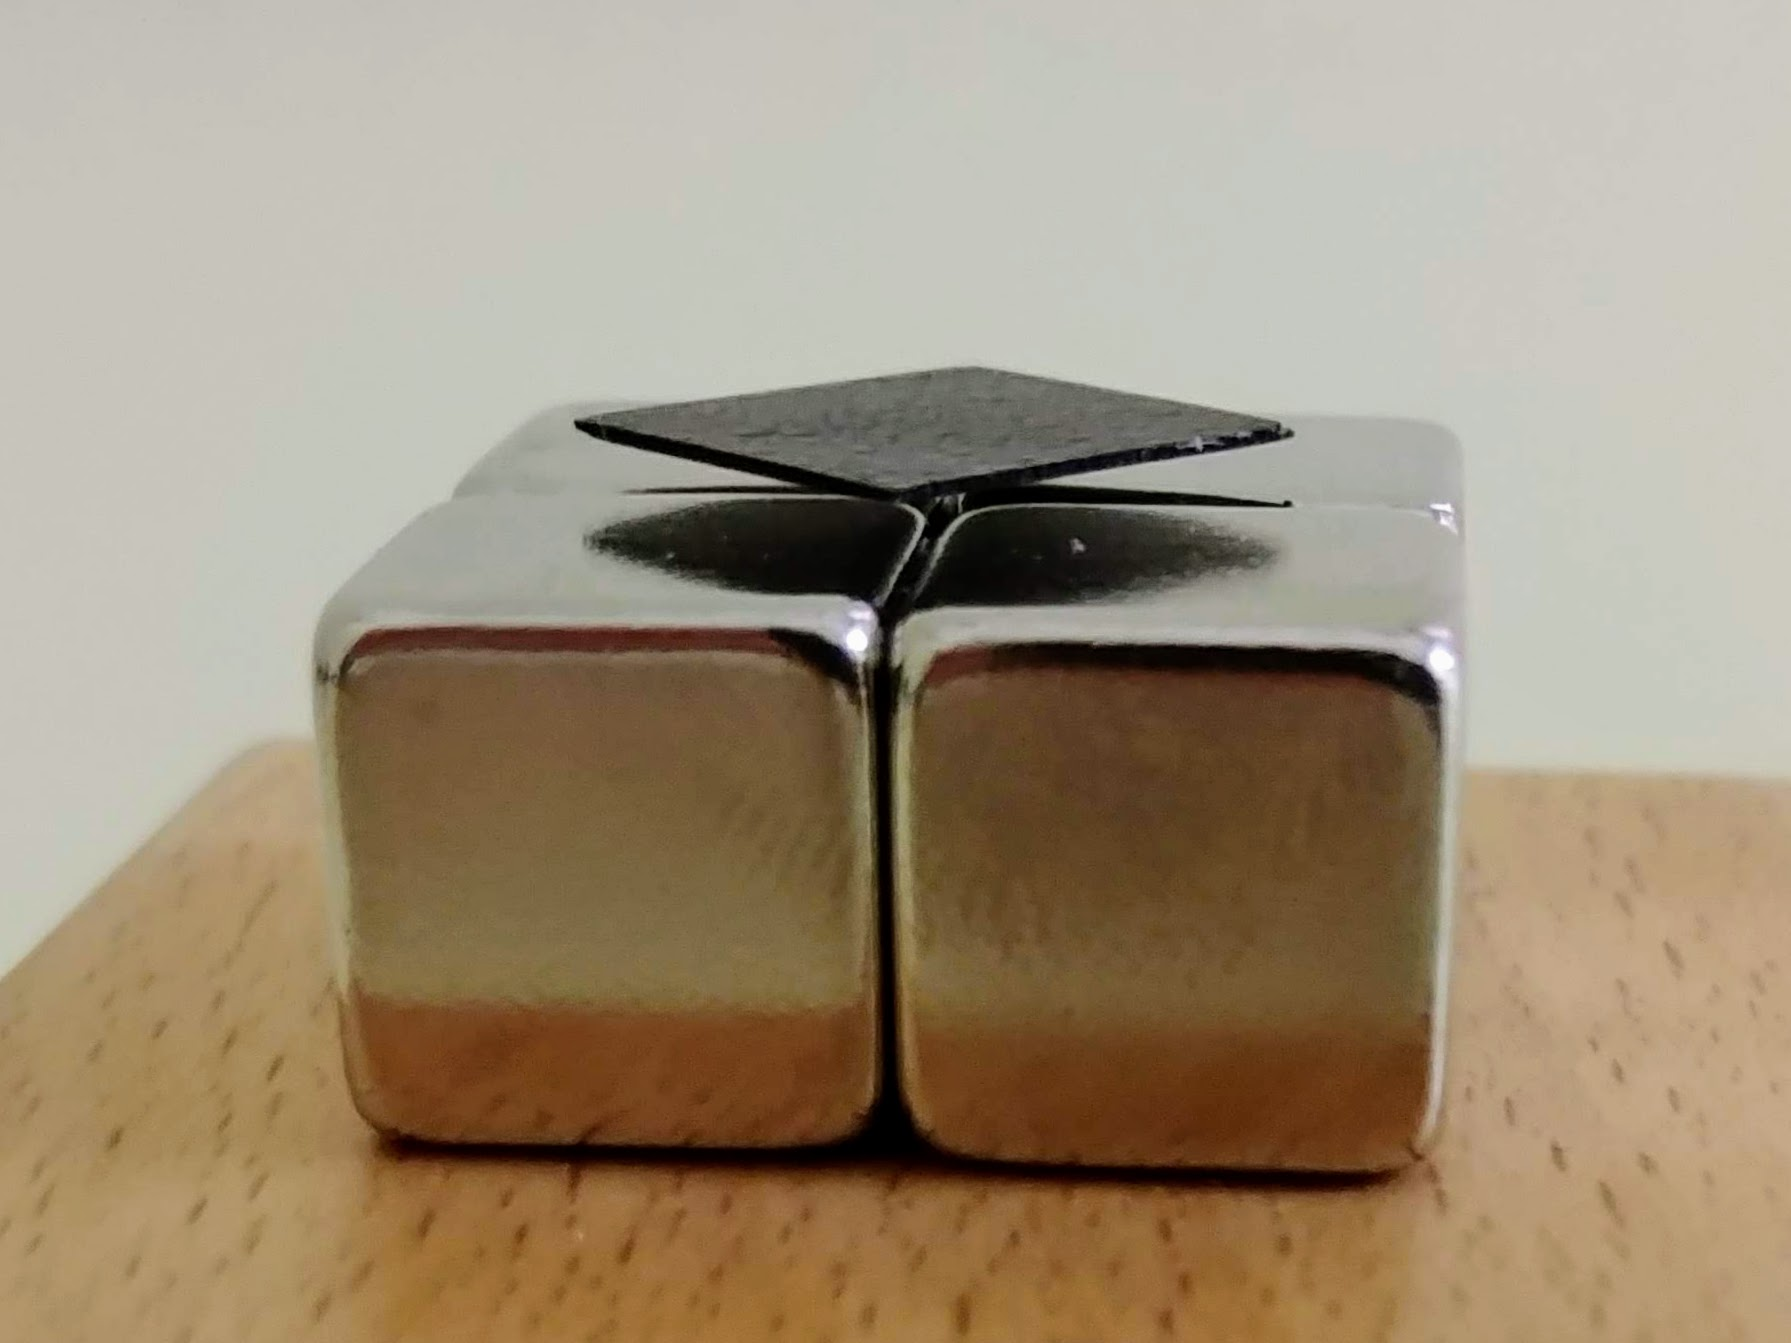
\includegraphics[width=.4\linewidth]{fig/experimentos/diamaglev_3}
	}
	\caption{Placa de grafito (diamagnético) levitando, a temperatura ambiente y sin aportes externos de energía, sobre cuatro imanes con polaridades alternantes. Los materiales diamagnéticos son repelidos por los campos magnéticos.}
\end{figure}
\end{frame}

\begin{frame}{Materiales ferromagnéticos y paramagnéticos}
\begin{columns}
	\column{0.6\textwidth}
	Las cerillas comunes tienen compuesto de óxido de hierro que es paramagnético.
	Cuando se prenden, este óxido de hierro sufre la siguiente transformación:
	$$
		\text{Fe}_2\text{O}_3 \rightarrow 2 \, \text{Fe} + 3 \, \text{O}_2
	$$
	El hierro que se obtiene es ferromagnético. Por tanto vemos que una cerilla prendida puede ser atraida por un imán.
	\column{0.4\textwidth}
	\begin{figure}
		\centering
		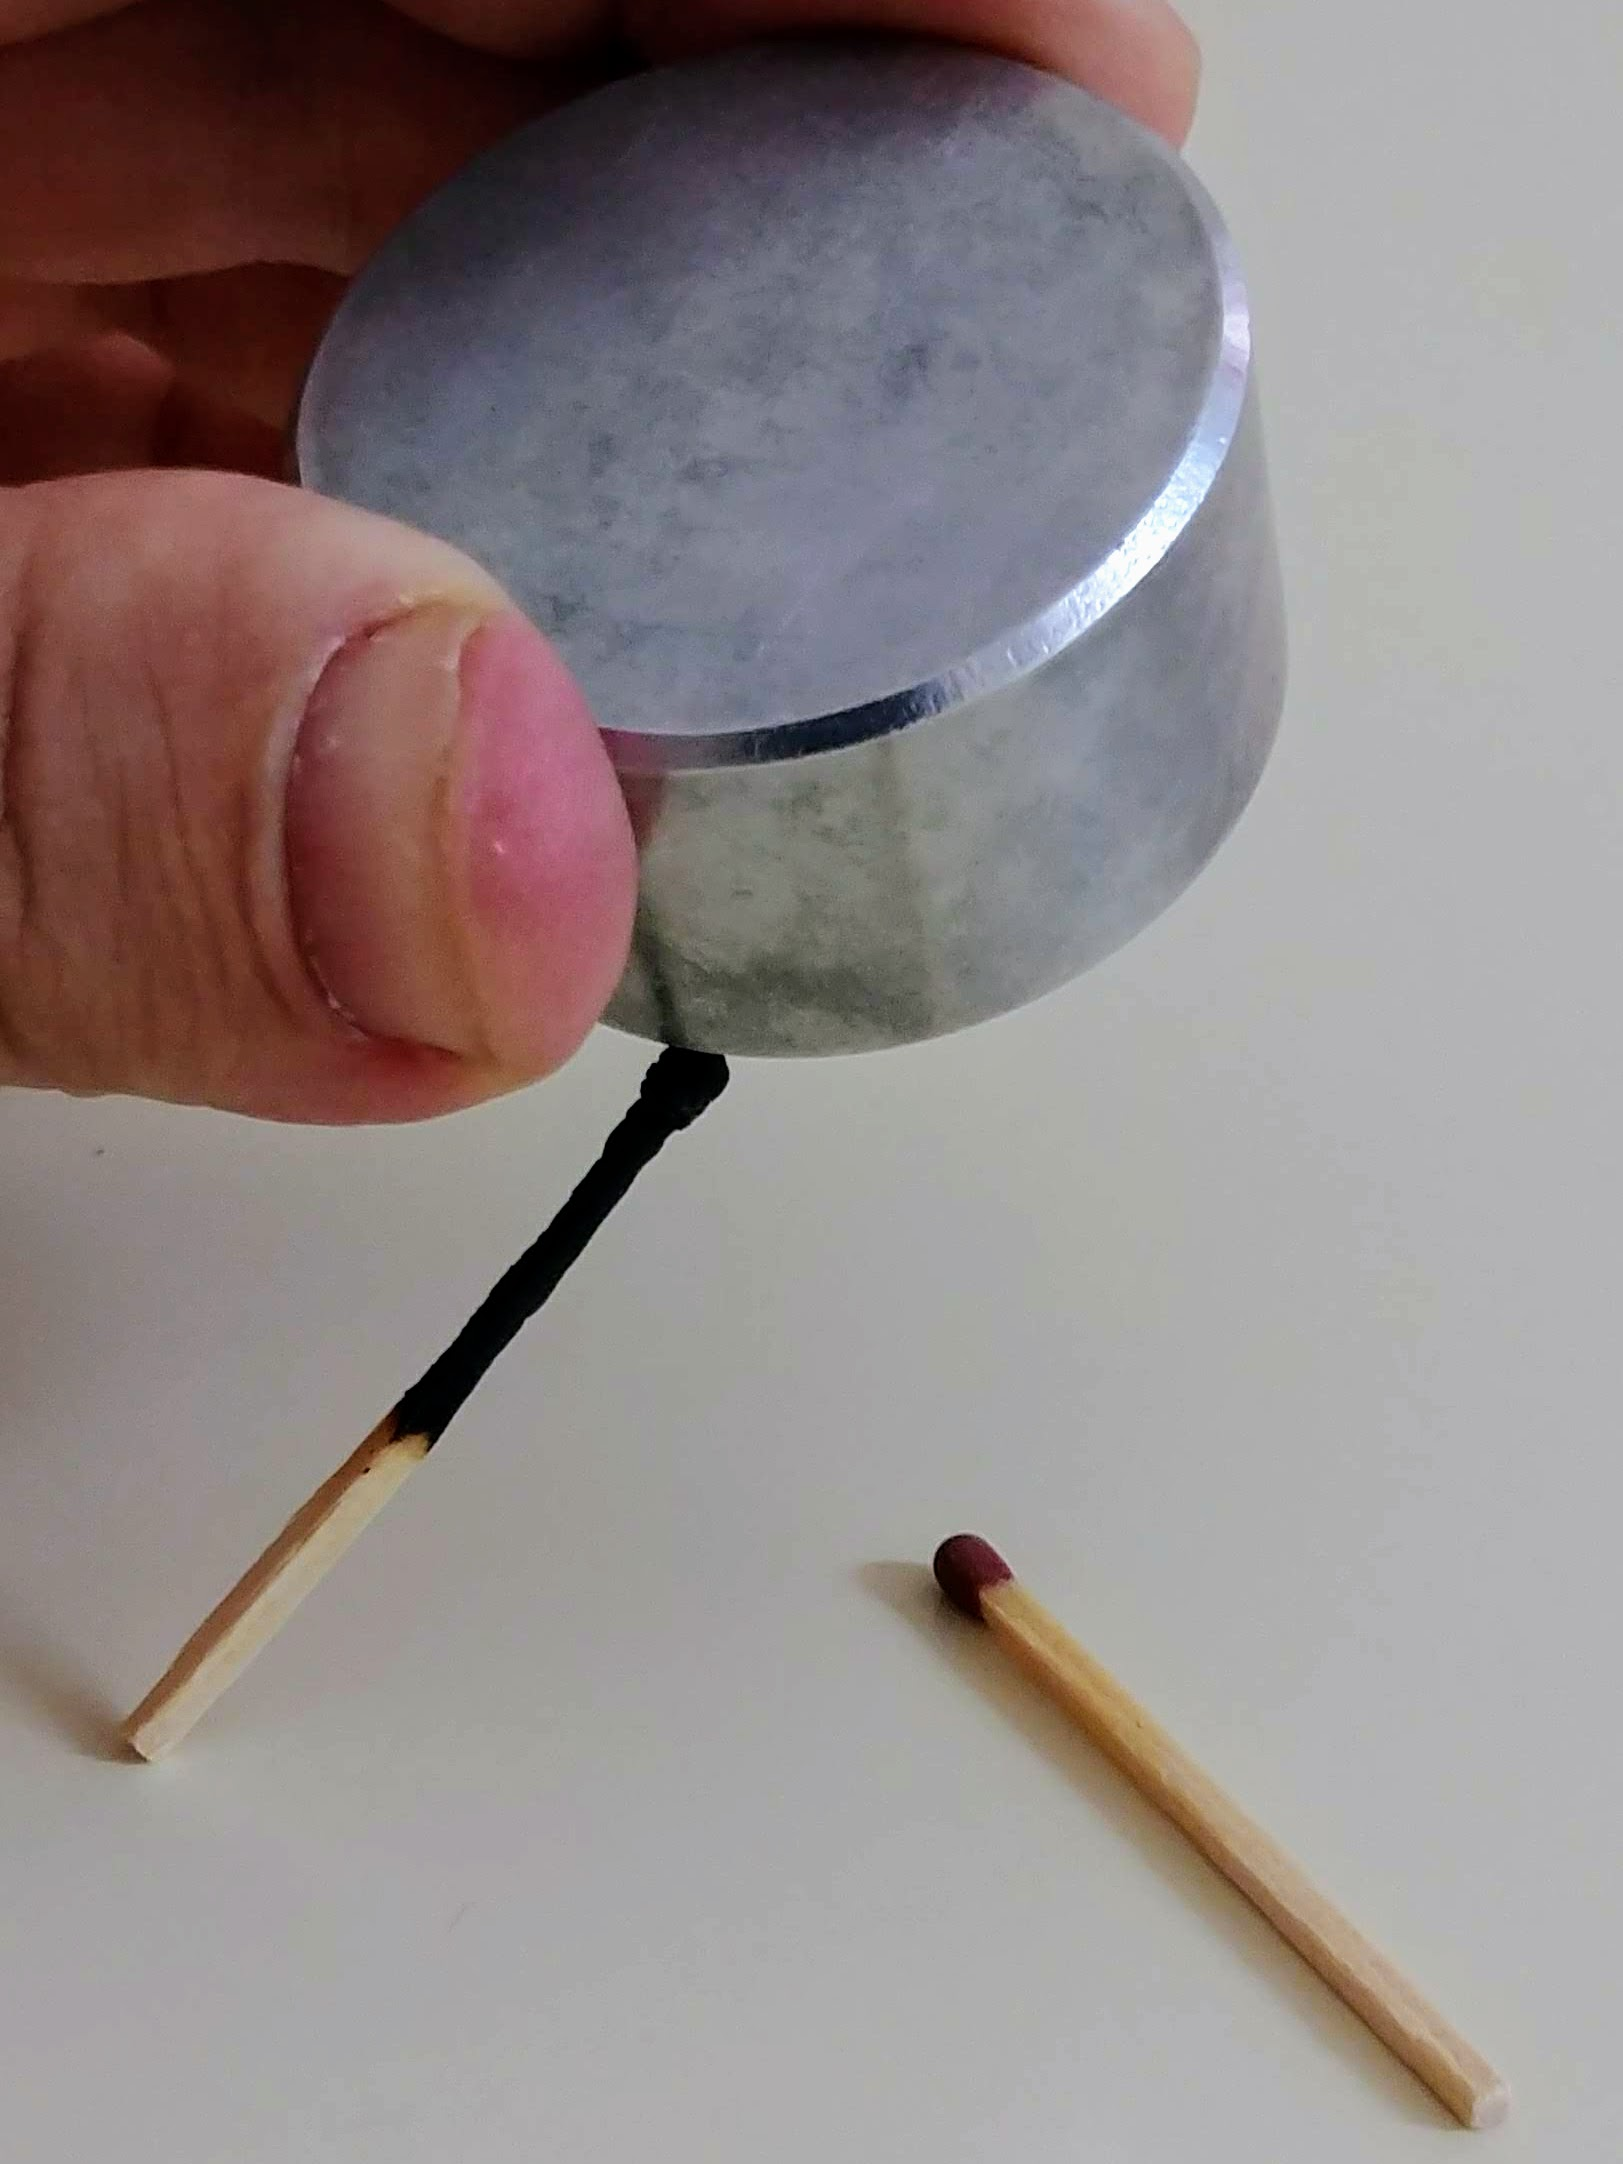
\includegraphics[width=1\linewidth]{fig/experimentos/iman_y_cerillas}
		\caption{Imán de neodimio y cerillas.}
	\end{figure}
\end{columns}
\end{frame}


\section{Corriente alterna}
\subsection{Introducción teórica}
\begin{frame}{Corriente alterna}
\begin{columns}
	\column{0.5\textwidth} 
	\justifying
	En una fuente de tensión alterna la tensión y la corriente varían sinusoidalmente con el tiempo:
	\begin{align}
	v(t) & = V \cos (\omega t) \nonumber\\
	i(t) & = I \cos (\omega t) \nonumber
	\end{align}
	donde $v$ e $i$ son la tensión y corriente \textbf{instantáneas} respectivamente. $V$ e $I$ representan los valores \textbf{máximos} de estas magnitudes    
	\column{0.5\textwidth}   
	\begin{center}
		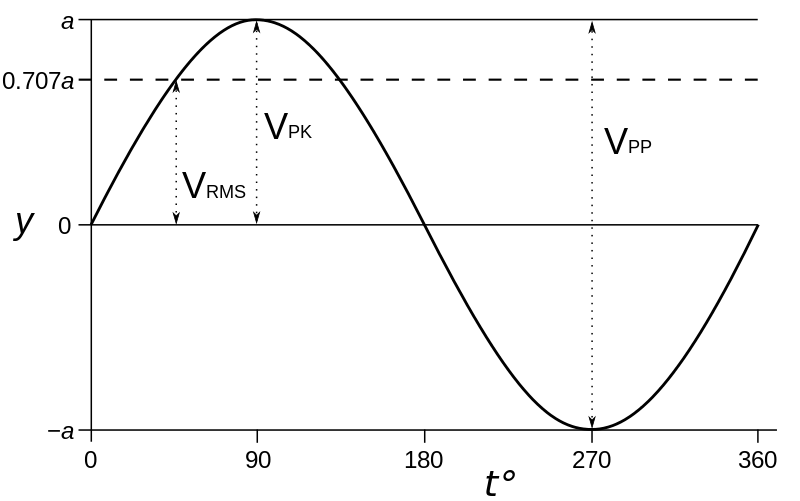
\includegraphics[width=1\linewidth]{voltaje_alterna}
	\end{center}
\end{columns}
\end{frame}

\subsection{Componentes pasivos en CA}
\begin{frame}
	La caida de tensión en una resistencia por la que circula una corriente alterna $i(t)$ viene dada por la ley de Ohm
	\begin{align}
	v_R (t) & = i(t) R = (IR) cos (\omega t) \nonumber \\
	V_R & = IR \nonumber
	\end{align}
	La corriente $i$ y el voltaje $v_R$ son proporcionales a a $\cos(\omega t)$, por tanto la \textbf{corriente está en fase con el voltaje}.   
	
	En un condensador, podemos obtener la carga integrando
	la corriente con respecto al tiempo
	$$
	q = \int i \, dt = \frac{I}{\omega} \sin (\omega t)
	$$
	teniendo en cuenta la fórmula de la capacidad, $C = q/V$,
	$$
	v_C = \frac{I}{\omega C} \sin(\omega t) 
	= \frac{I}{\omega C} \cos(\omega t - \pi/2)
	$$
\end{frame}

\subsection{Diseño experimental}
\begin{frame}
\begin{columns}
	\column{0.6\textwidth}
	\justifying
	Las bolas de plasma funcionan mediante de corriente alterna. Esta corriente pasa por un gas que al ionizarse emite un destello luminoso. Al ser alterna, esta corriente puede atravesar el cristal de la esfera mediante un mecanismo capacitivo,
	$$
		i(t) = C \frac{d v(t)}{d t}
	$$
	
	Las corrientes cierran el circuito (vuelven a tierra) a través del aire o de nuestro propio cuerpo. Al acercar una lámpara fluorescente podemos observar que se enciende ya que las corrientes pueden atravesar también el cristal de la lámpara.
	\column{0.4\textwidth}
	\begin{figure}
		\centering
		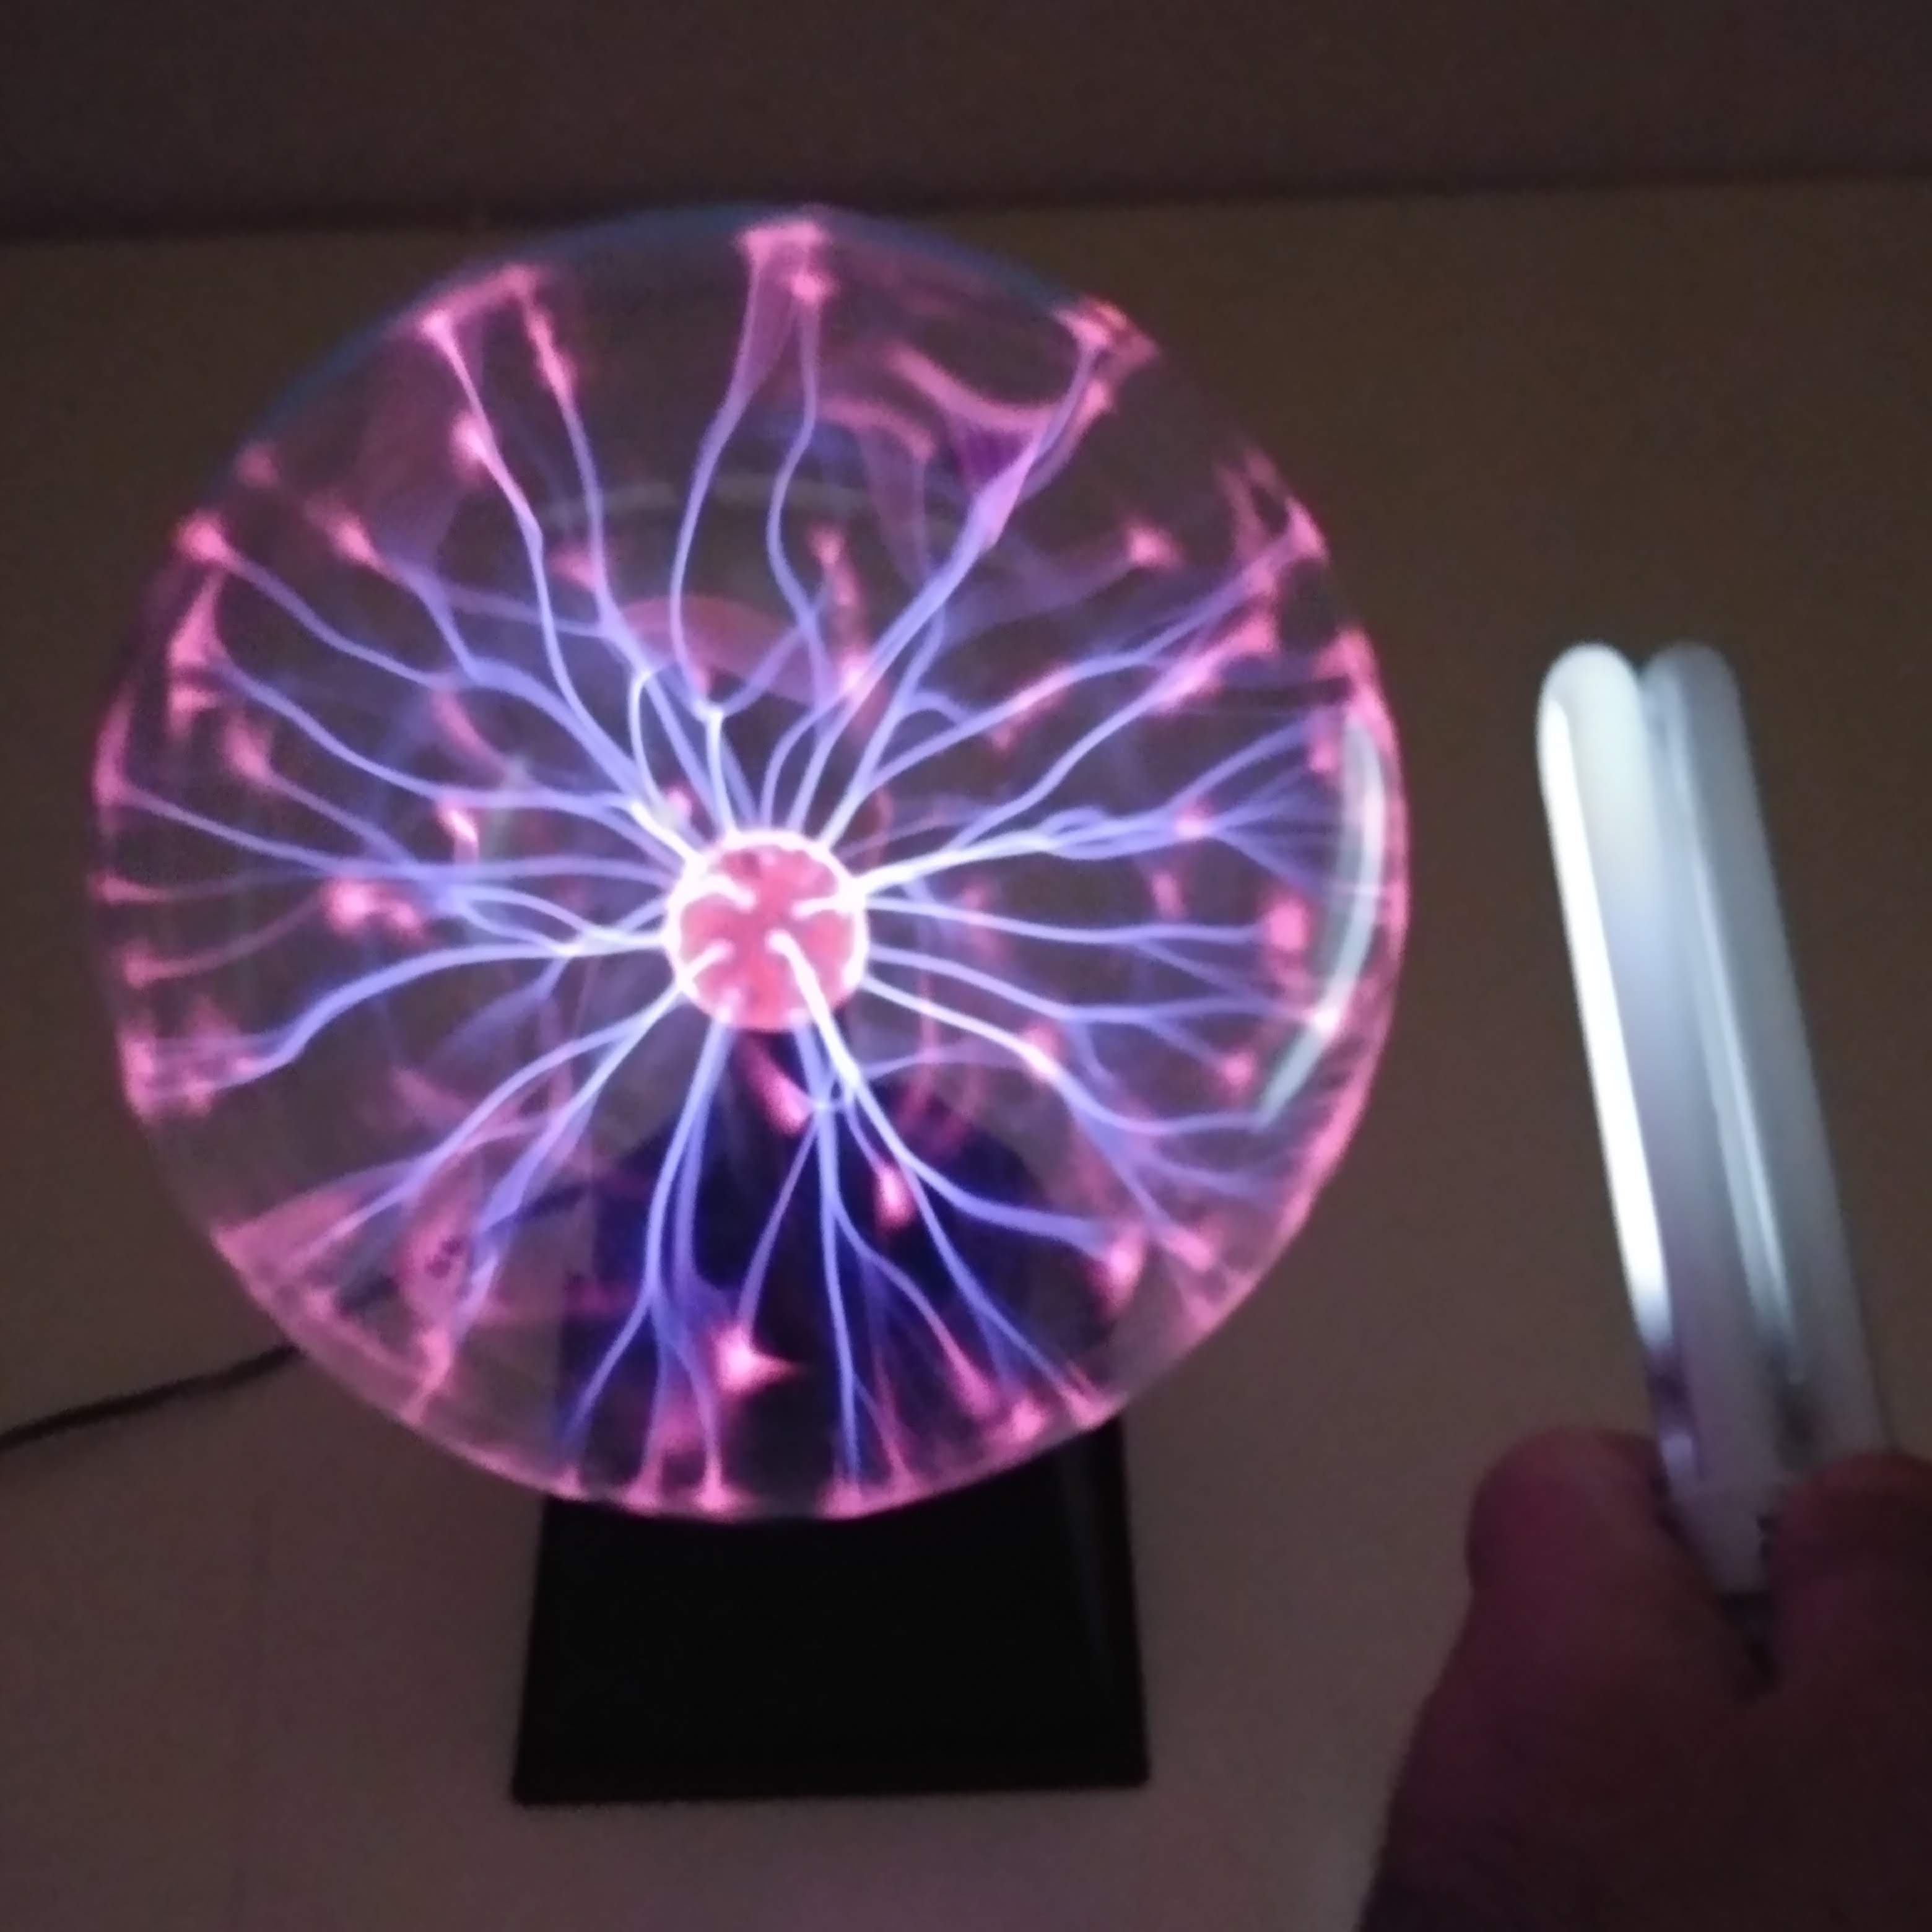
\includegraphics[width=1\linewidth]{fig/experimentos/bola_de_plasma_y_bombilla}
		\caption{\centering Lámpara de plasma y bombilla fluorescente}
	\end{figure}
\end{columns}
\end{frame}

\section{Reconstrucción de un arcoiris en el aula}
\subsection{Introducción teórica}
\begin{frame}{Dispersión de la luz}
La \textbf{dispersión} de la luz es un fenómeno que se produce cuando \textbf{un rayo de luz compuesta} se refracta en algún medio (por ejemplo un prisma), quedando separados sus colores constituyentes.
\begin{columns}
	\column{0.5\textwidth}
	\begin{figure}
		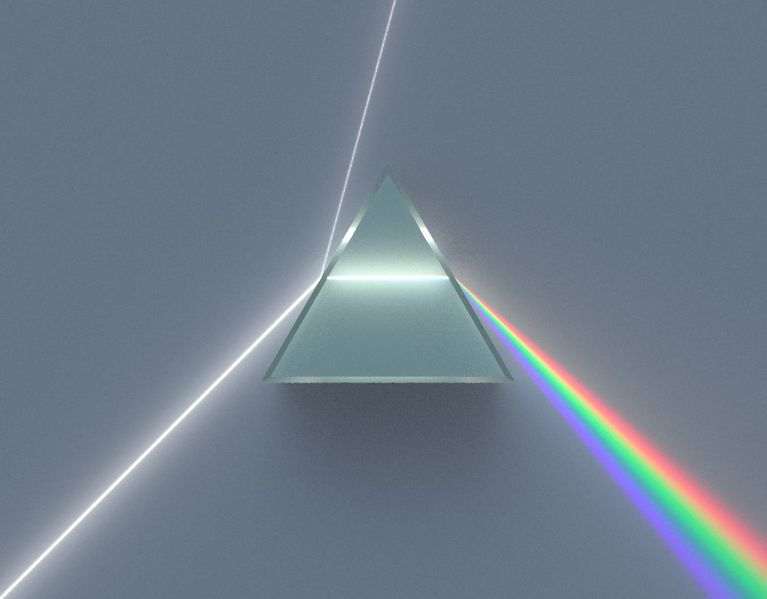
\includegraphics[width=1\textwidth]{prism}
		\caption{\tiny Fuente: Wikipedia, CC BY-SA 3.0}
	\end{figure}
	\column{0.5\textwidth}      
	\begin{figure}
		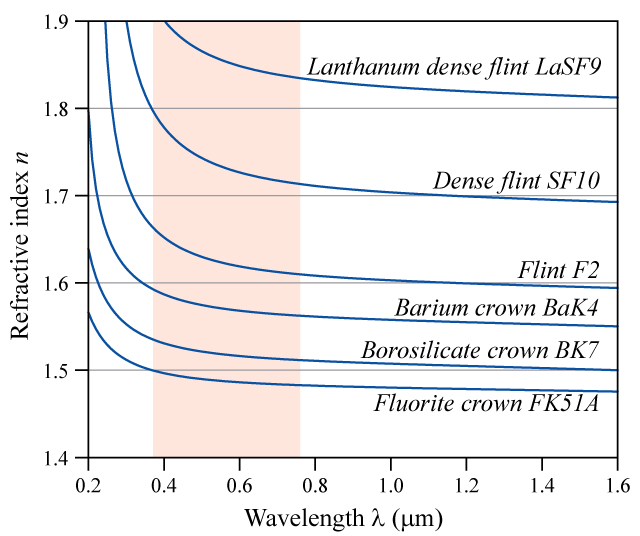
\includegraphics[width=\textwidth]{indicesRefraccionFrecuencia.png}
		\caption{\tiny Fuente: Wikipedia, CC BY-SA 3.0}
	\end{figure}
\end{columns}
\end{frame}

\begin{frame}{Arco iris}
\begin{figure}
	\centering
	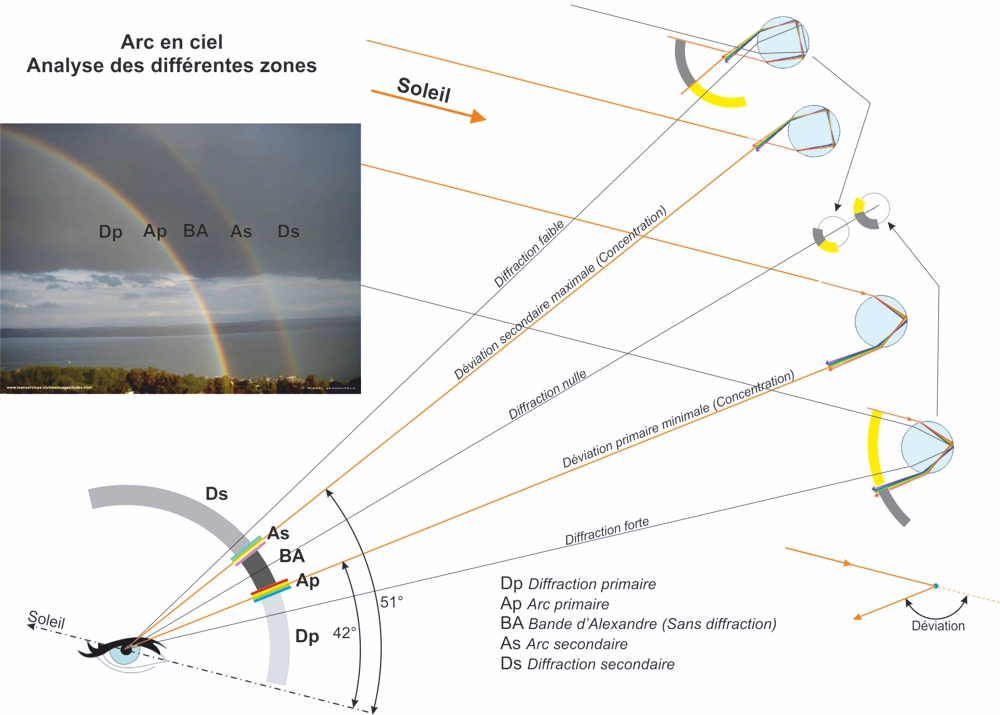
\includegraphics[width=.8\linewidth]{Arc_en_ciel_synthese-red.jpg}
	\caption{\tiny Fuente: Wikipedia, CC BY-SA 3.0}
\end{figure}
\end{frame}

\subsection{Diseño experimental}
\begin{frame}{Materiales}
\begin{figure}
	\centering
	\subfloat[Esfera de vidrio y lasers de colores rojo, verde, y azul]{
		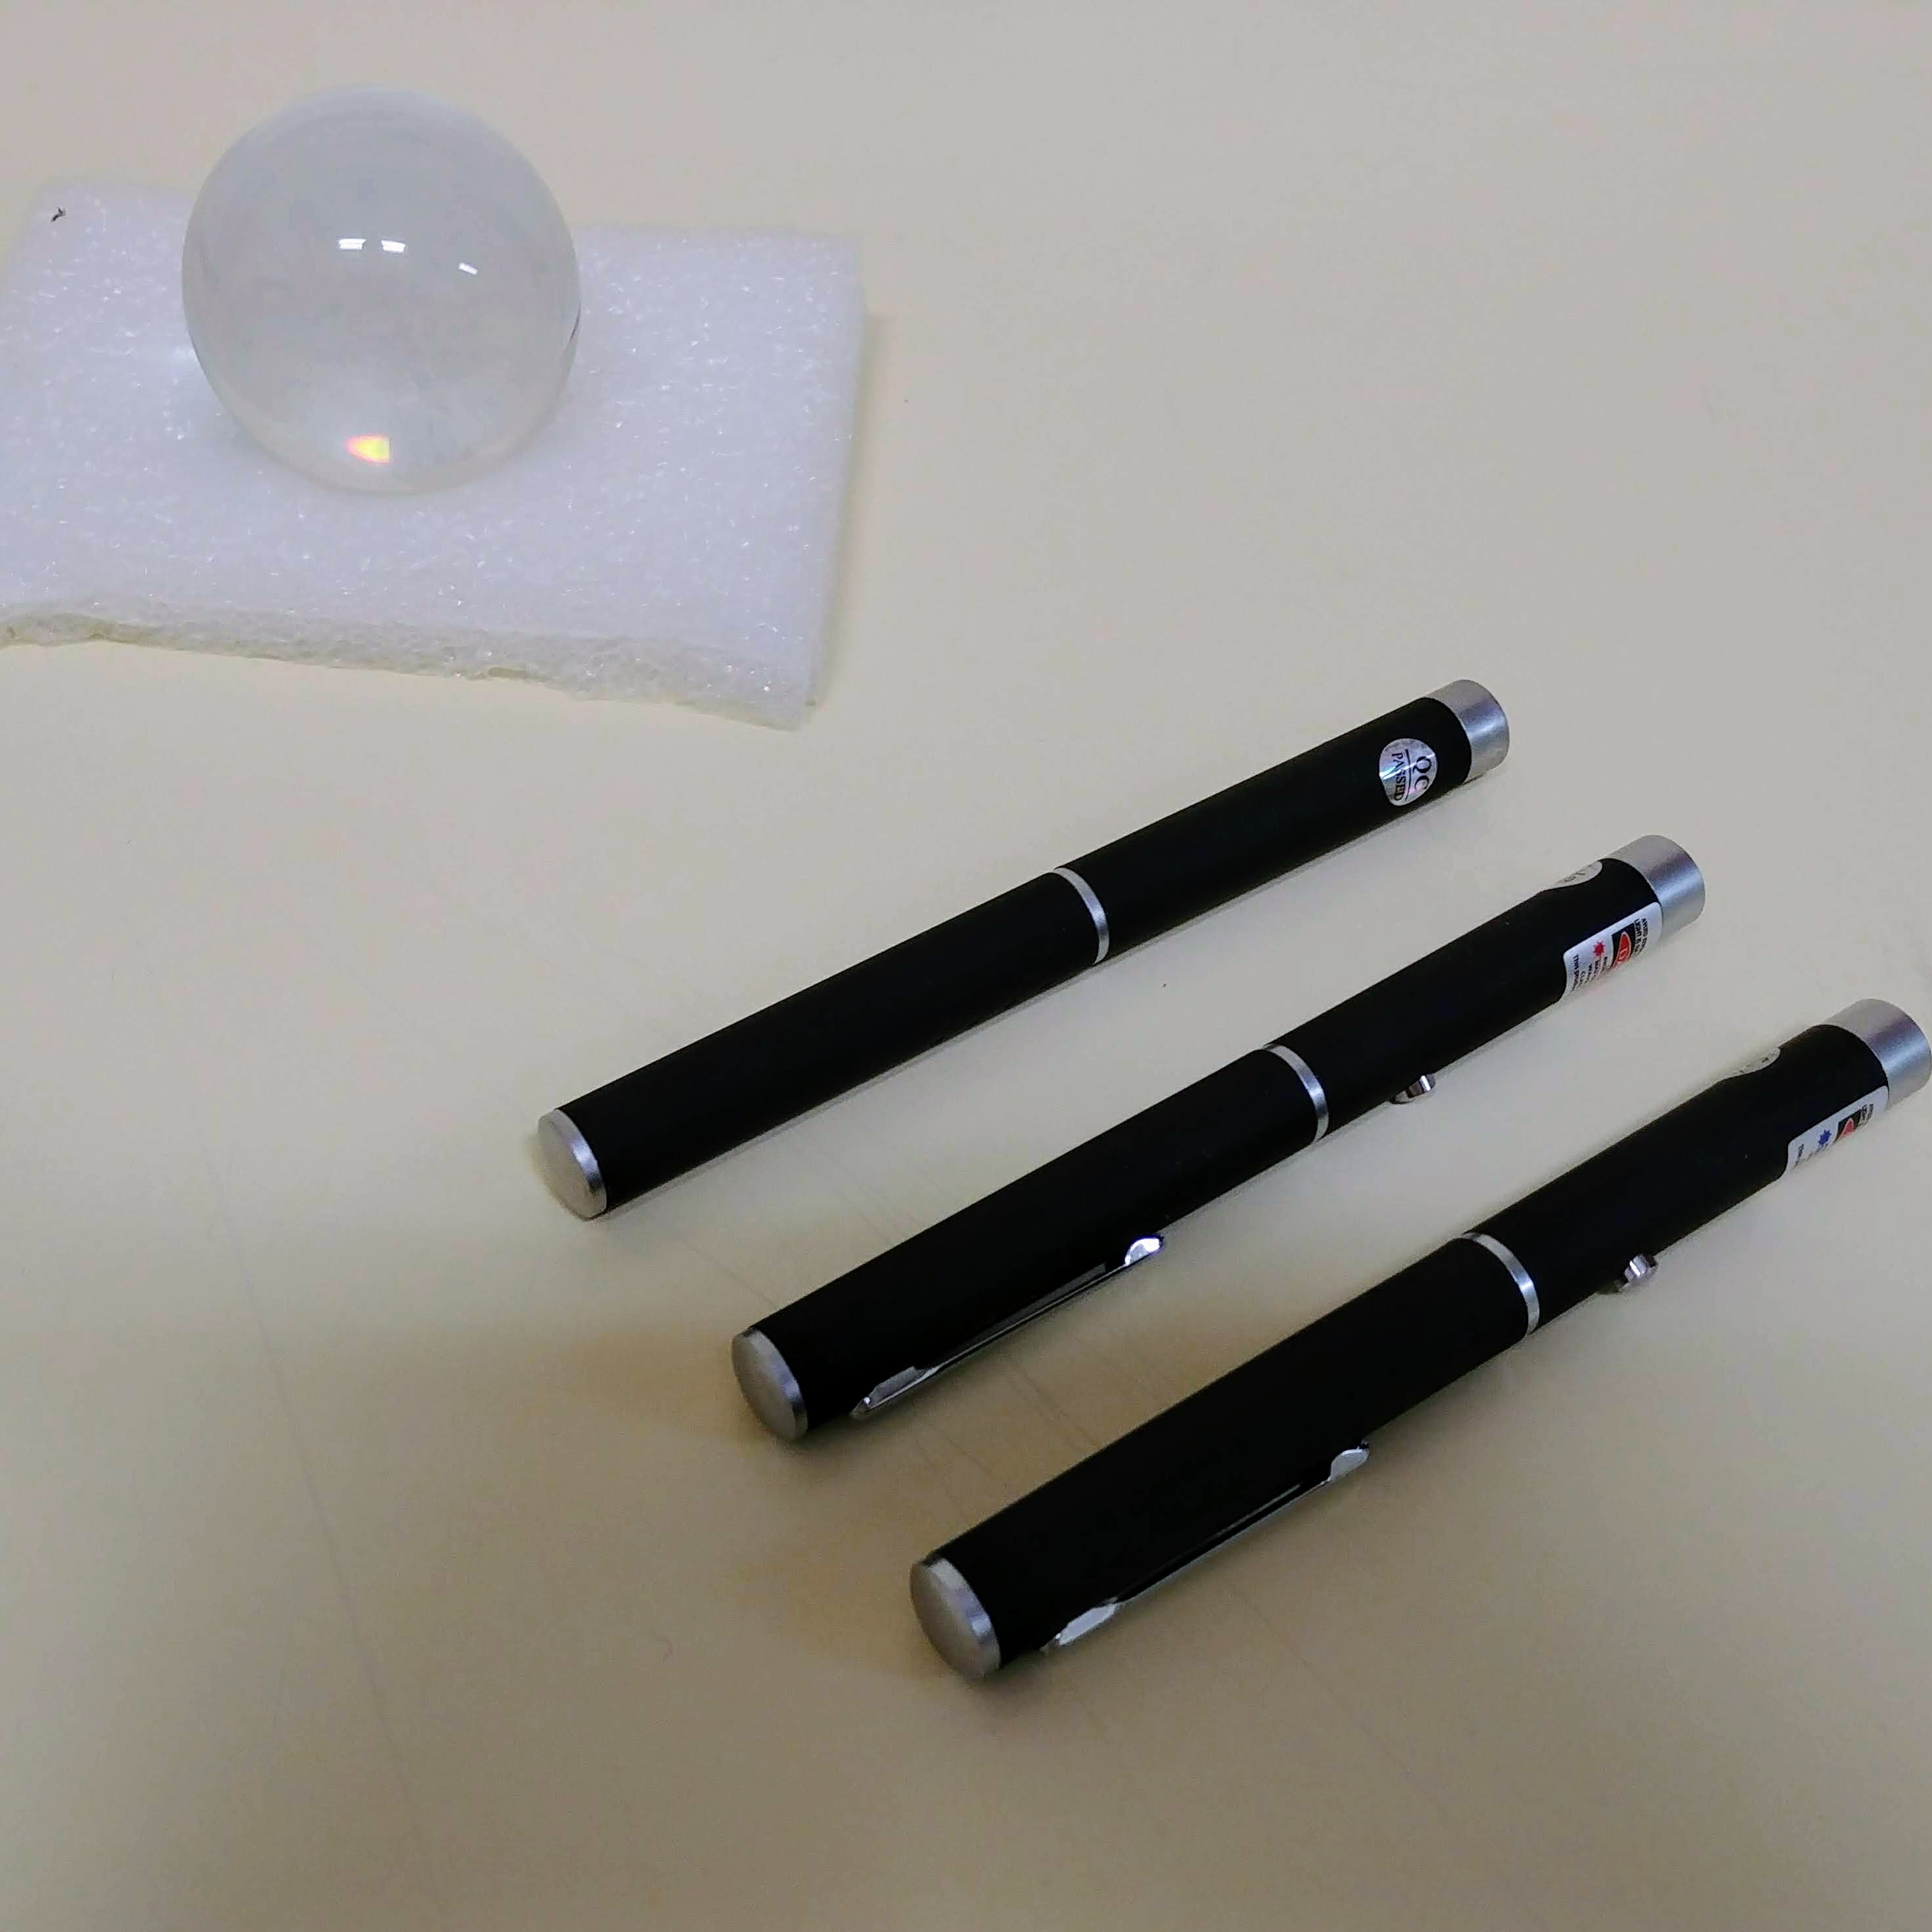
\includegraphics[width=.27\linewidth]{fig/experimentos/arcoiris_esfera_cristal_y_lasers}
	}\,
	\subfloat[Reflexión interna total dentro de la esfera de vidrio]{
		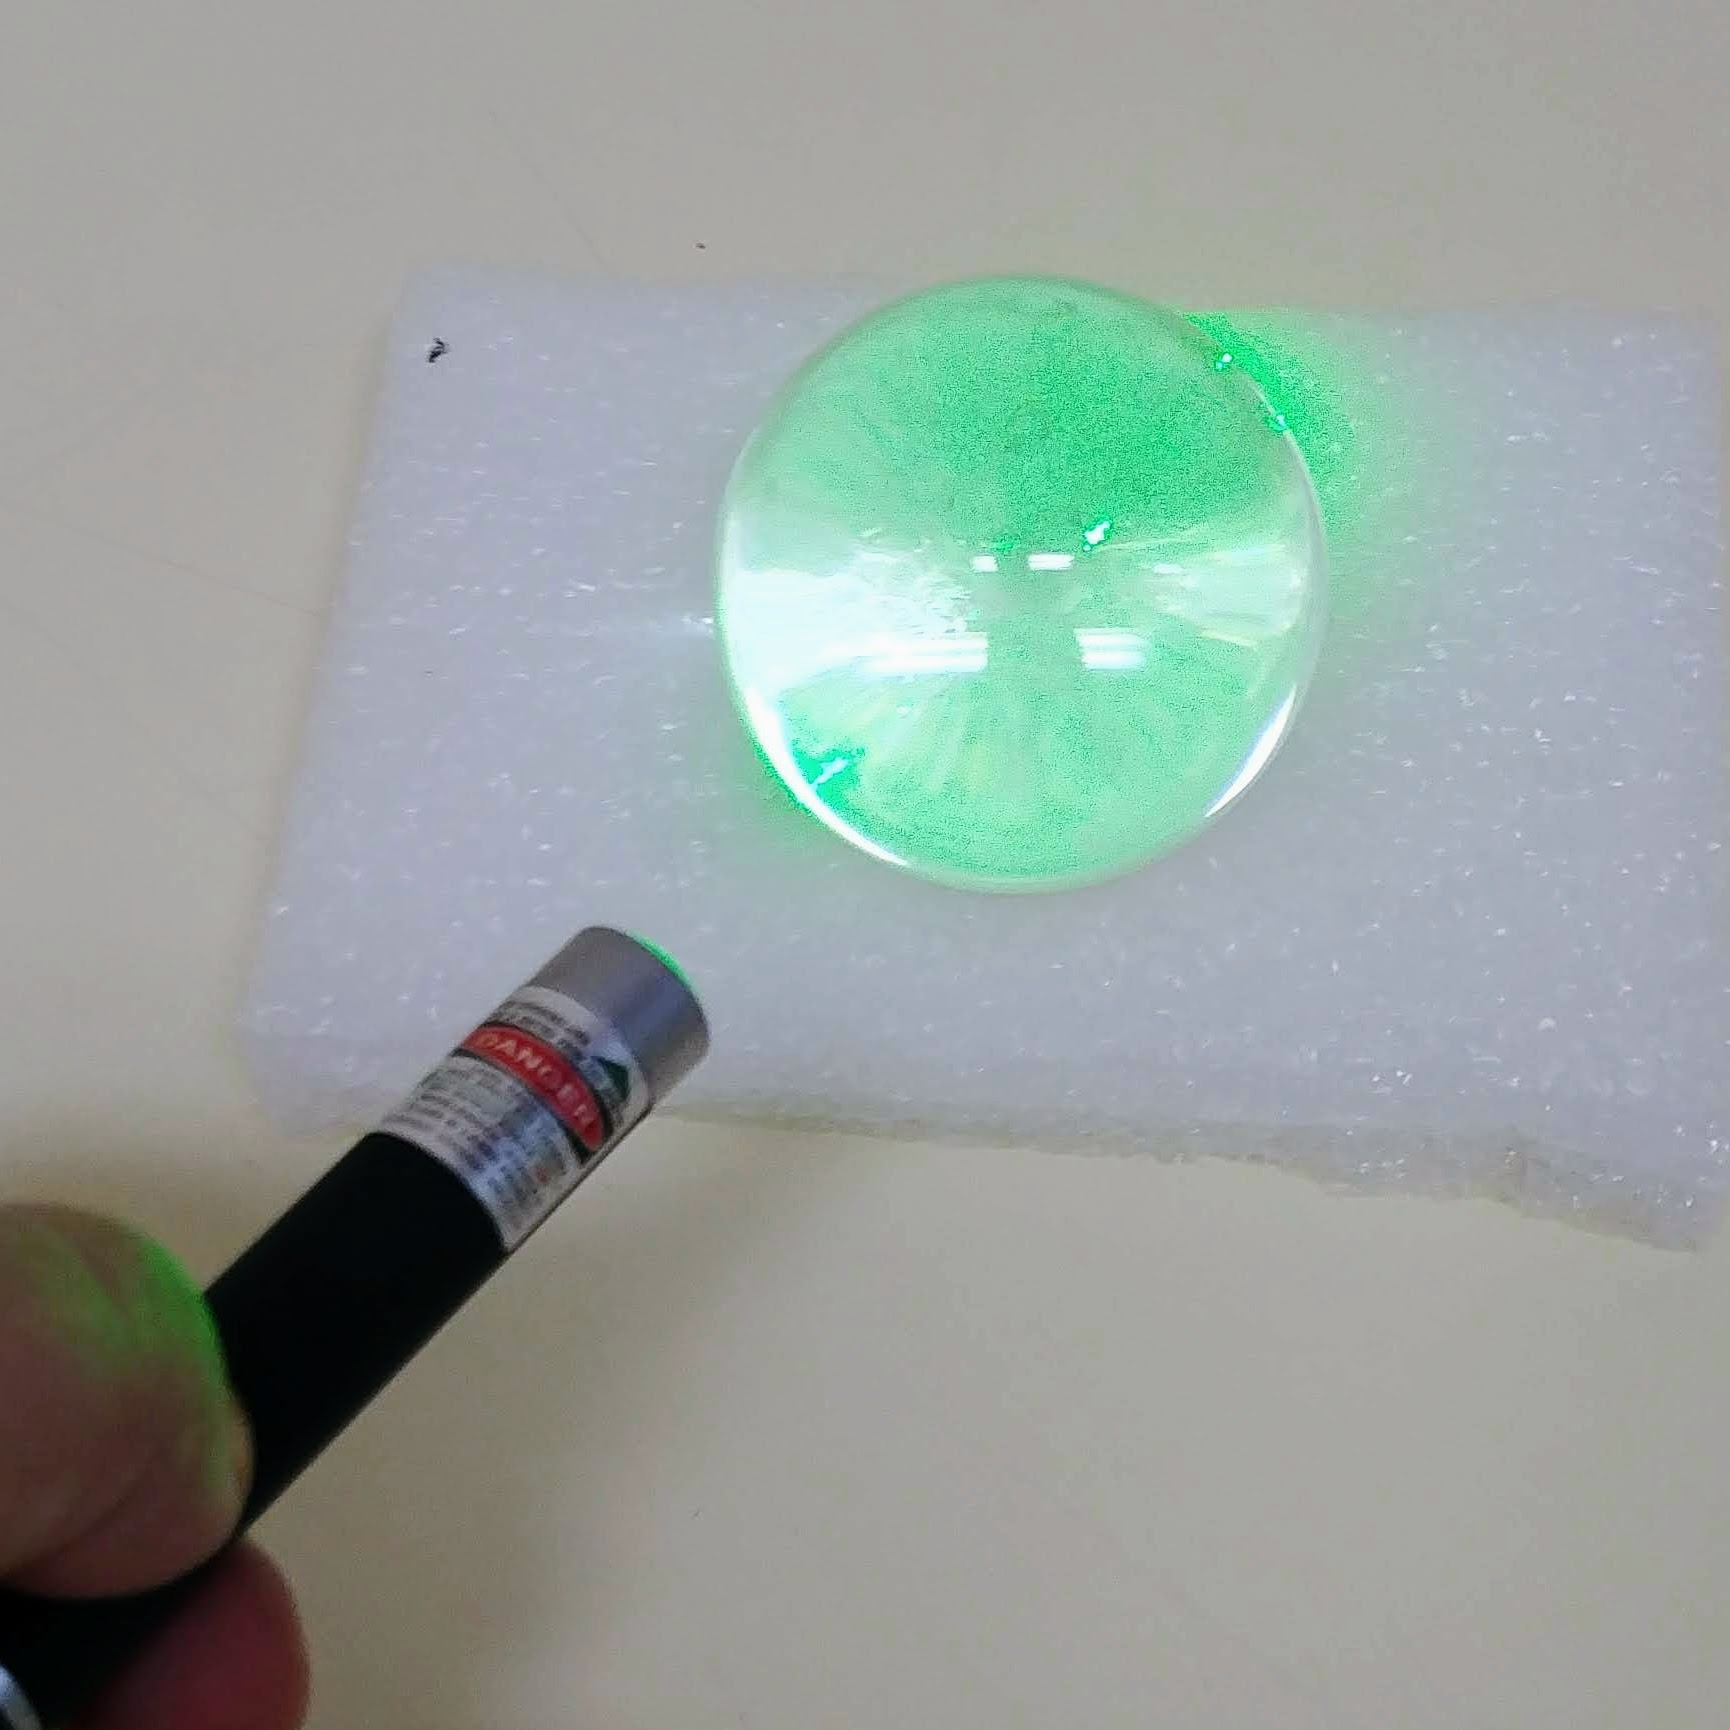
\includegraphics[width=.27\linewidth]{fig/experimentos/arcoiris_reflexion_1}
	}\,
	\subfloat[Reflexión dentro de la esfera de vidrio]{
		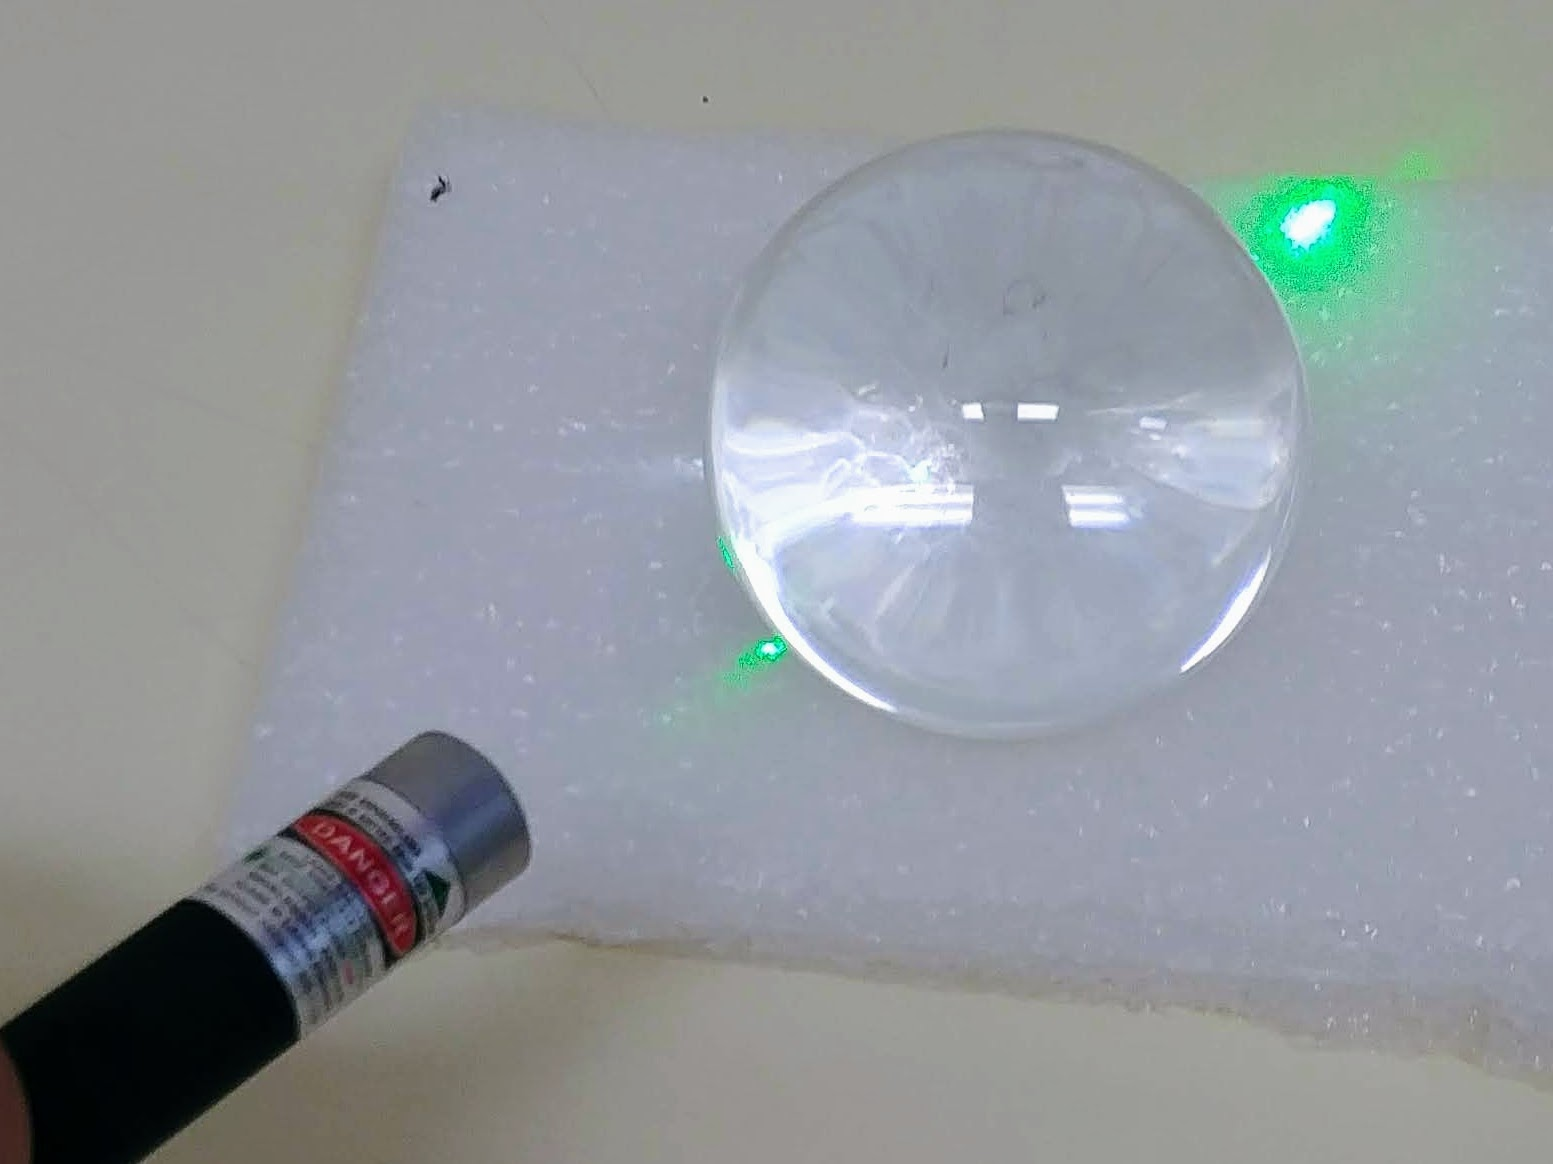
\includegraphics[width=.35\linewidth]{fig/experimentos/arcoiris_reflexion_2}
	}
	\caption{La esfera de vidrio sirve de modelo de gota de lluvia en la que se pueden estudiar la reflexión de la luz que da lugar al arcoiris. Los distintos haces de luz laser se refractan con ángulos distintos dando lugar a reflexiones internas en puntos distintos.}
\end{figure}
\end{frame}

\section{Polarización de la luz}
\subsection{Introducción teórica}
\begin{frame}{Polarización}
	Cuando el campo eléctrico de una onda está contenido a lo largo de un eje, se dice que la onda está \textbf{linealmente polarizada}.
	En general, si existe un patrón definido para describir el $\vec{E}$, hablamos de \textbf{luz polarizada}. En fuentes naturales, las oem son una superposición de muchas fuentes polarizadas aleatoriamente, a este tipo de luz se le llama \textbf{luz natural} o luz no polarizada.
\end{frame}

\begin{frame}{Filtros polarizadores}
	Es posible polarizar la luz natural mediante el uso de \textbf{filtros polarizadores}. Los filtros más comunes son materiales o sustancias con \textbf{dicroísmo} que impiden el paso de ondas en una orientación (\textbf{eje de polarización}) y lo permiten en otro.
	
	Algunas configuraciones geométricas también pueden actuar polarizando la luz. Por ejemplo una rejilla de alambres orientados, puede polarizar las oem de microondas.
	\begin{center}
		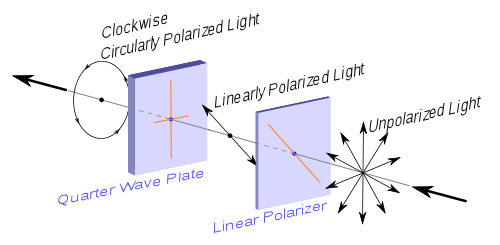
\includegraphics[width=.7\linewidth]{filtroPolarizador}
	\end{center}
\end{frame}

\begin{frame}
	La intensidad de luz que pasa por un filtro polarizador que forma un ángulo con su plano de polarización y descrita mediante la \textbf{ley de Malus}
	$$
	I = I_\text{máx} \cos^2 (\theta_1 - \theta_0)
	$$
	\begin{columns}
		\column{0.5\textwidth}
		\begin{figure}
			\centering	
			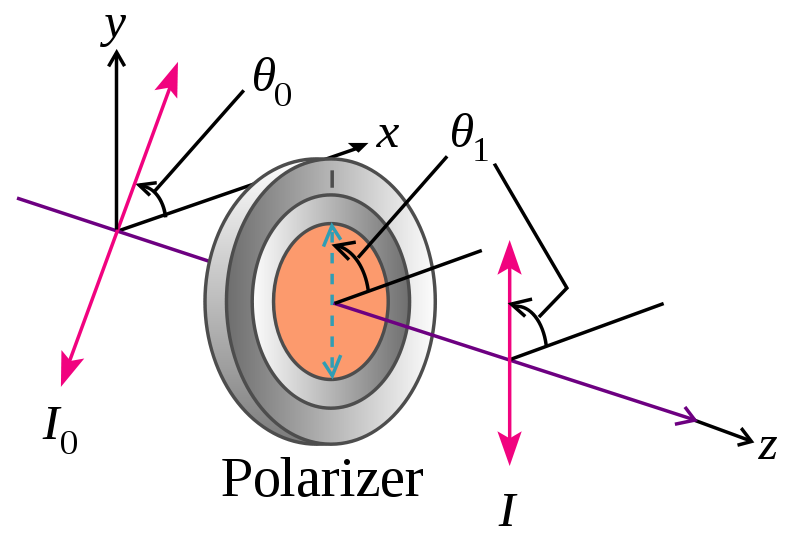
\includegraphics[width=1\textwidth]{doble_polarizacion}
			\caption{\tiny Fuente: Wikipedia, CC BY-SA 3.0}
		\end{figure}
		\column{0.5\textwidth}
		\begin{figure}
			\centering
			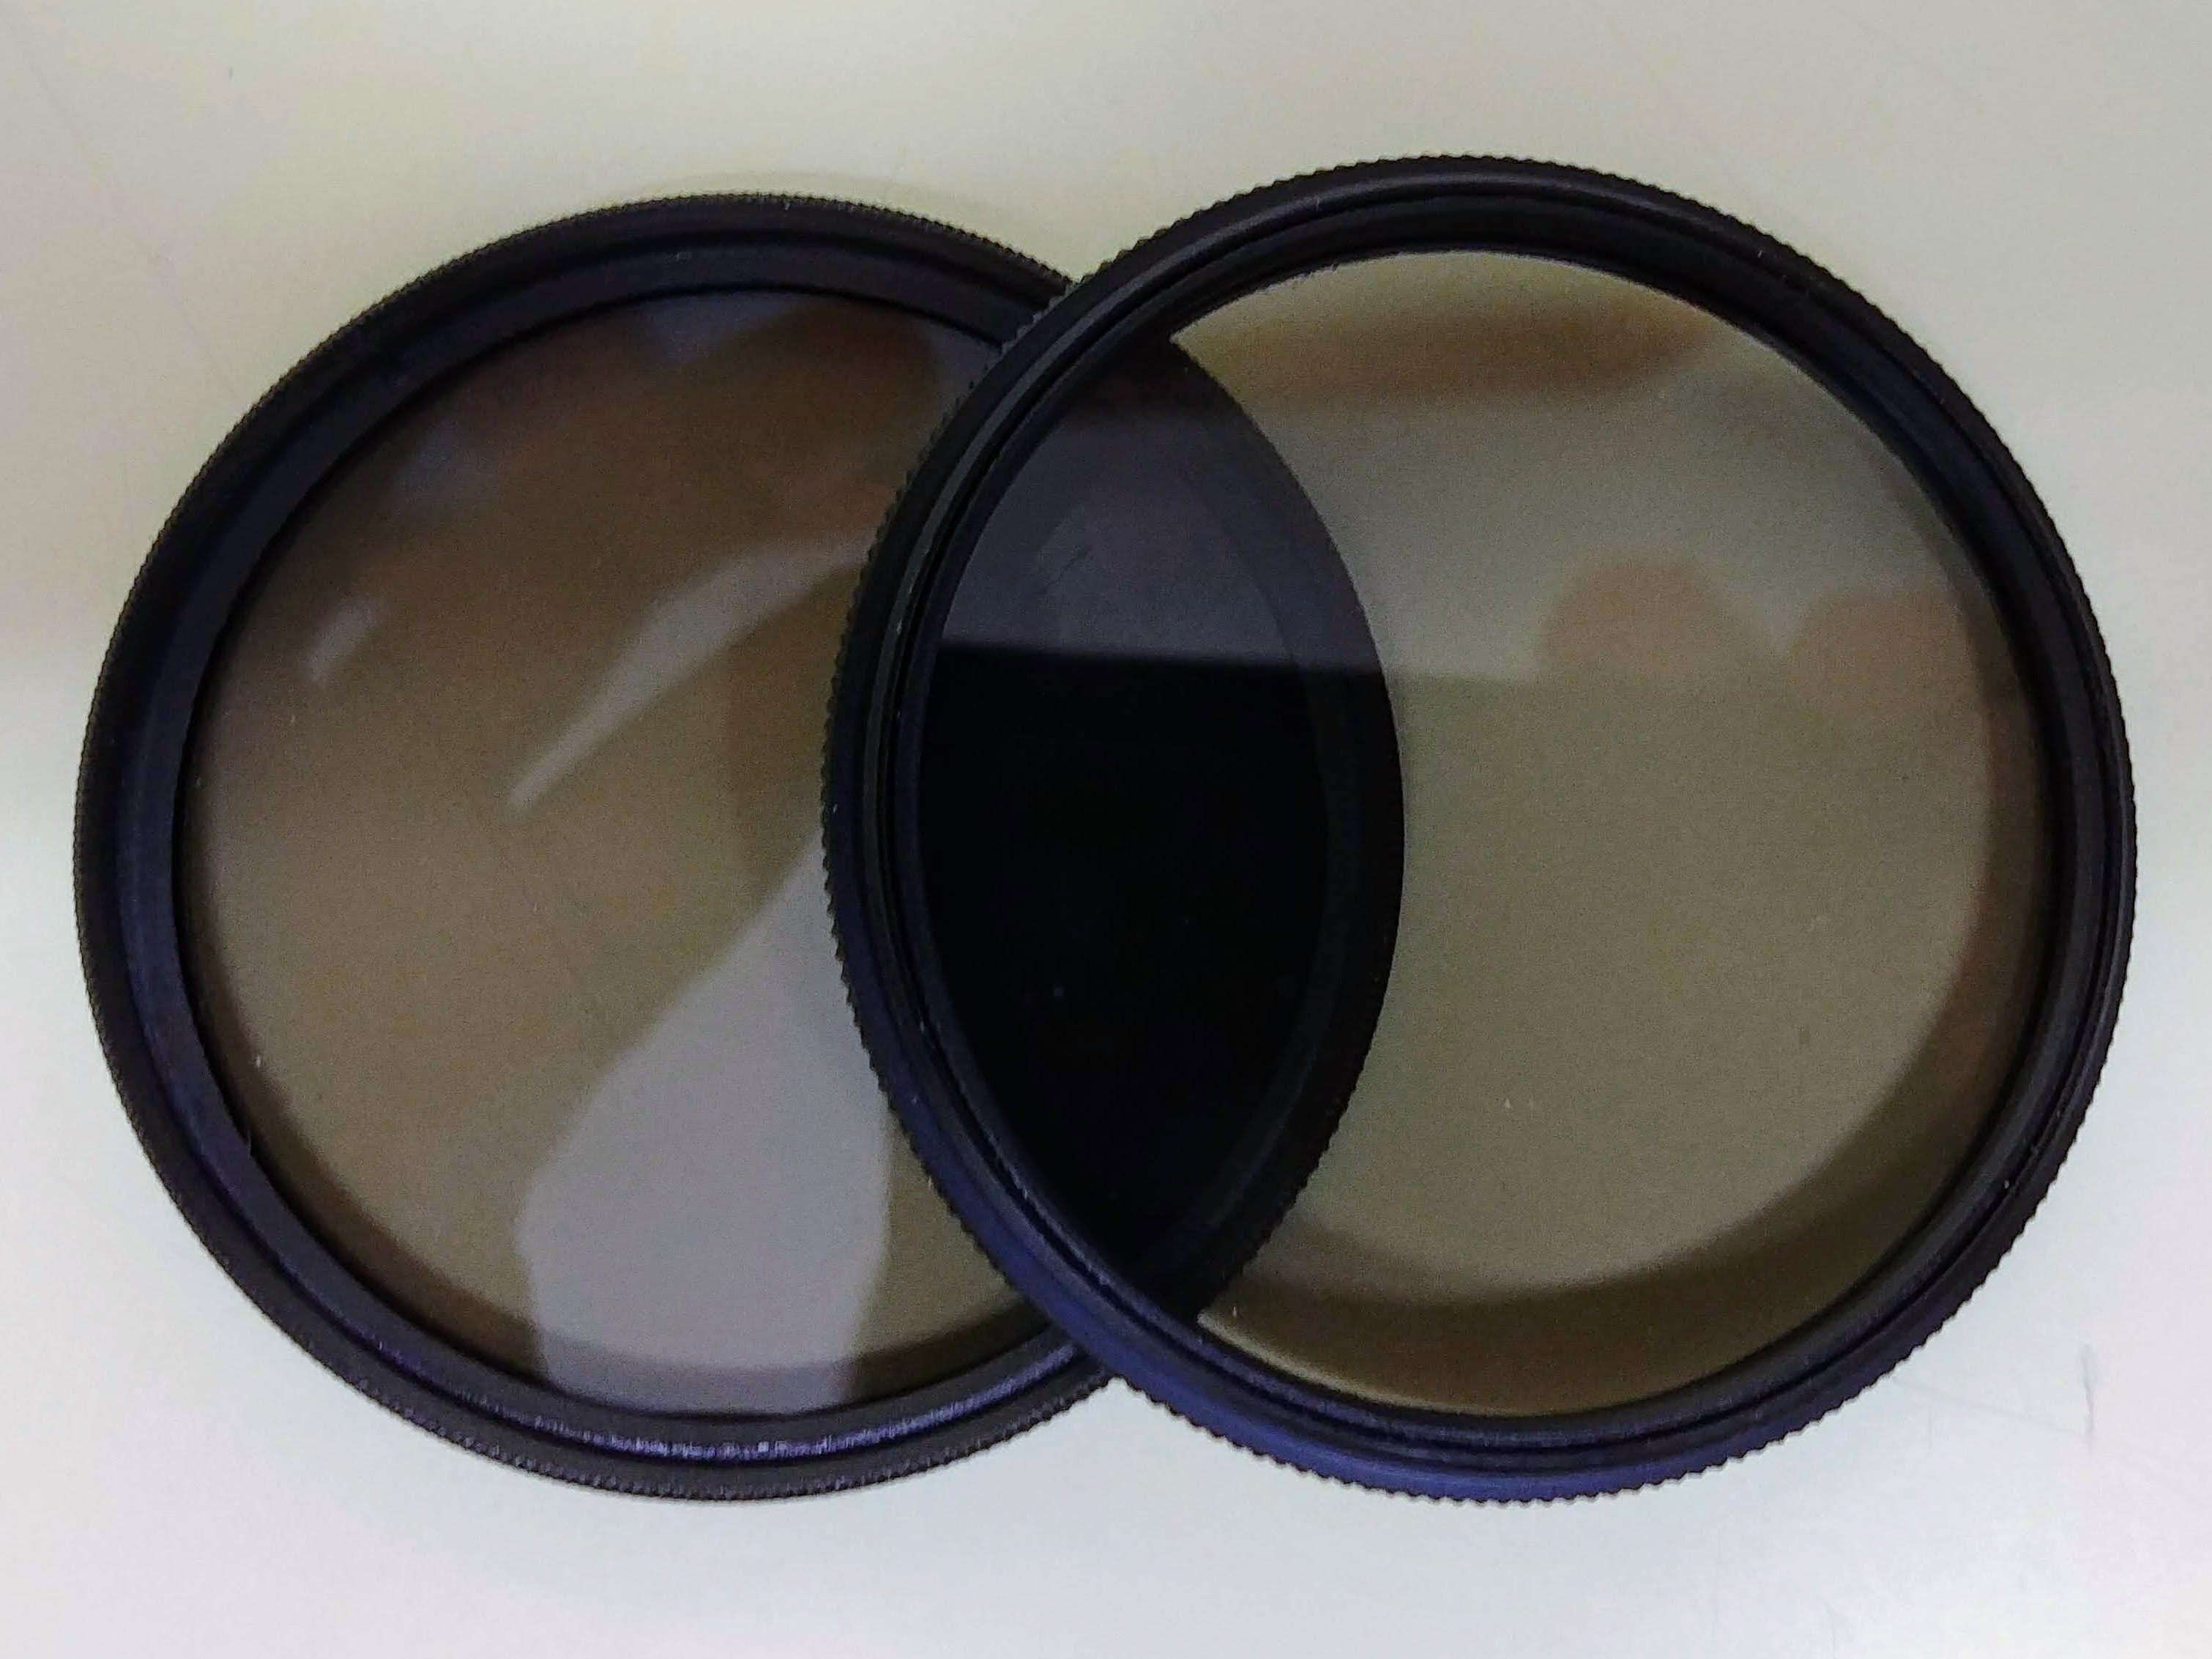
\includegraphics[width=.9\textwidth]{fig/experimentos/polarizacion_ley_de_malus}
			\caption{\justifying Filtros polarizadores formando un ángulo de $90^\circ$ entre sus ejes de polarización}
		\end{figure}
	\end{columns}
\end{frame}

\subsection{Diseño experimental}
\begin{frame}{Filtro de polarización}
\begin{figure}
	\centering
	\subfloat[$\phi = 0^\circ$]{
		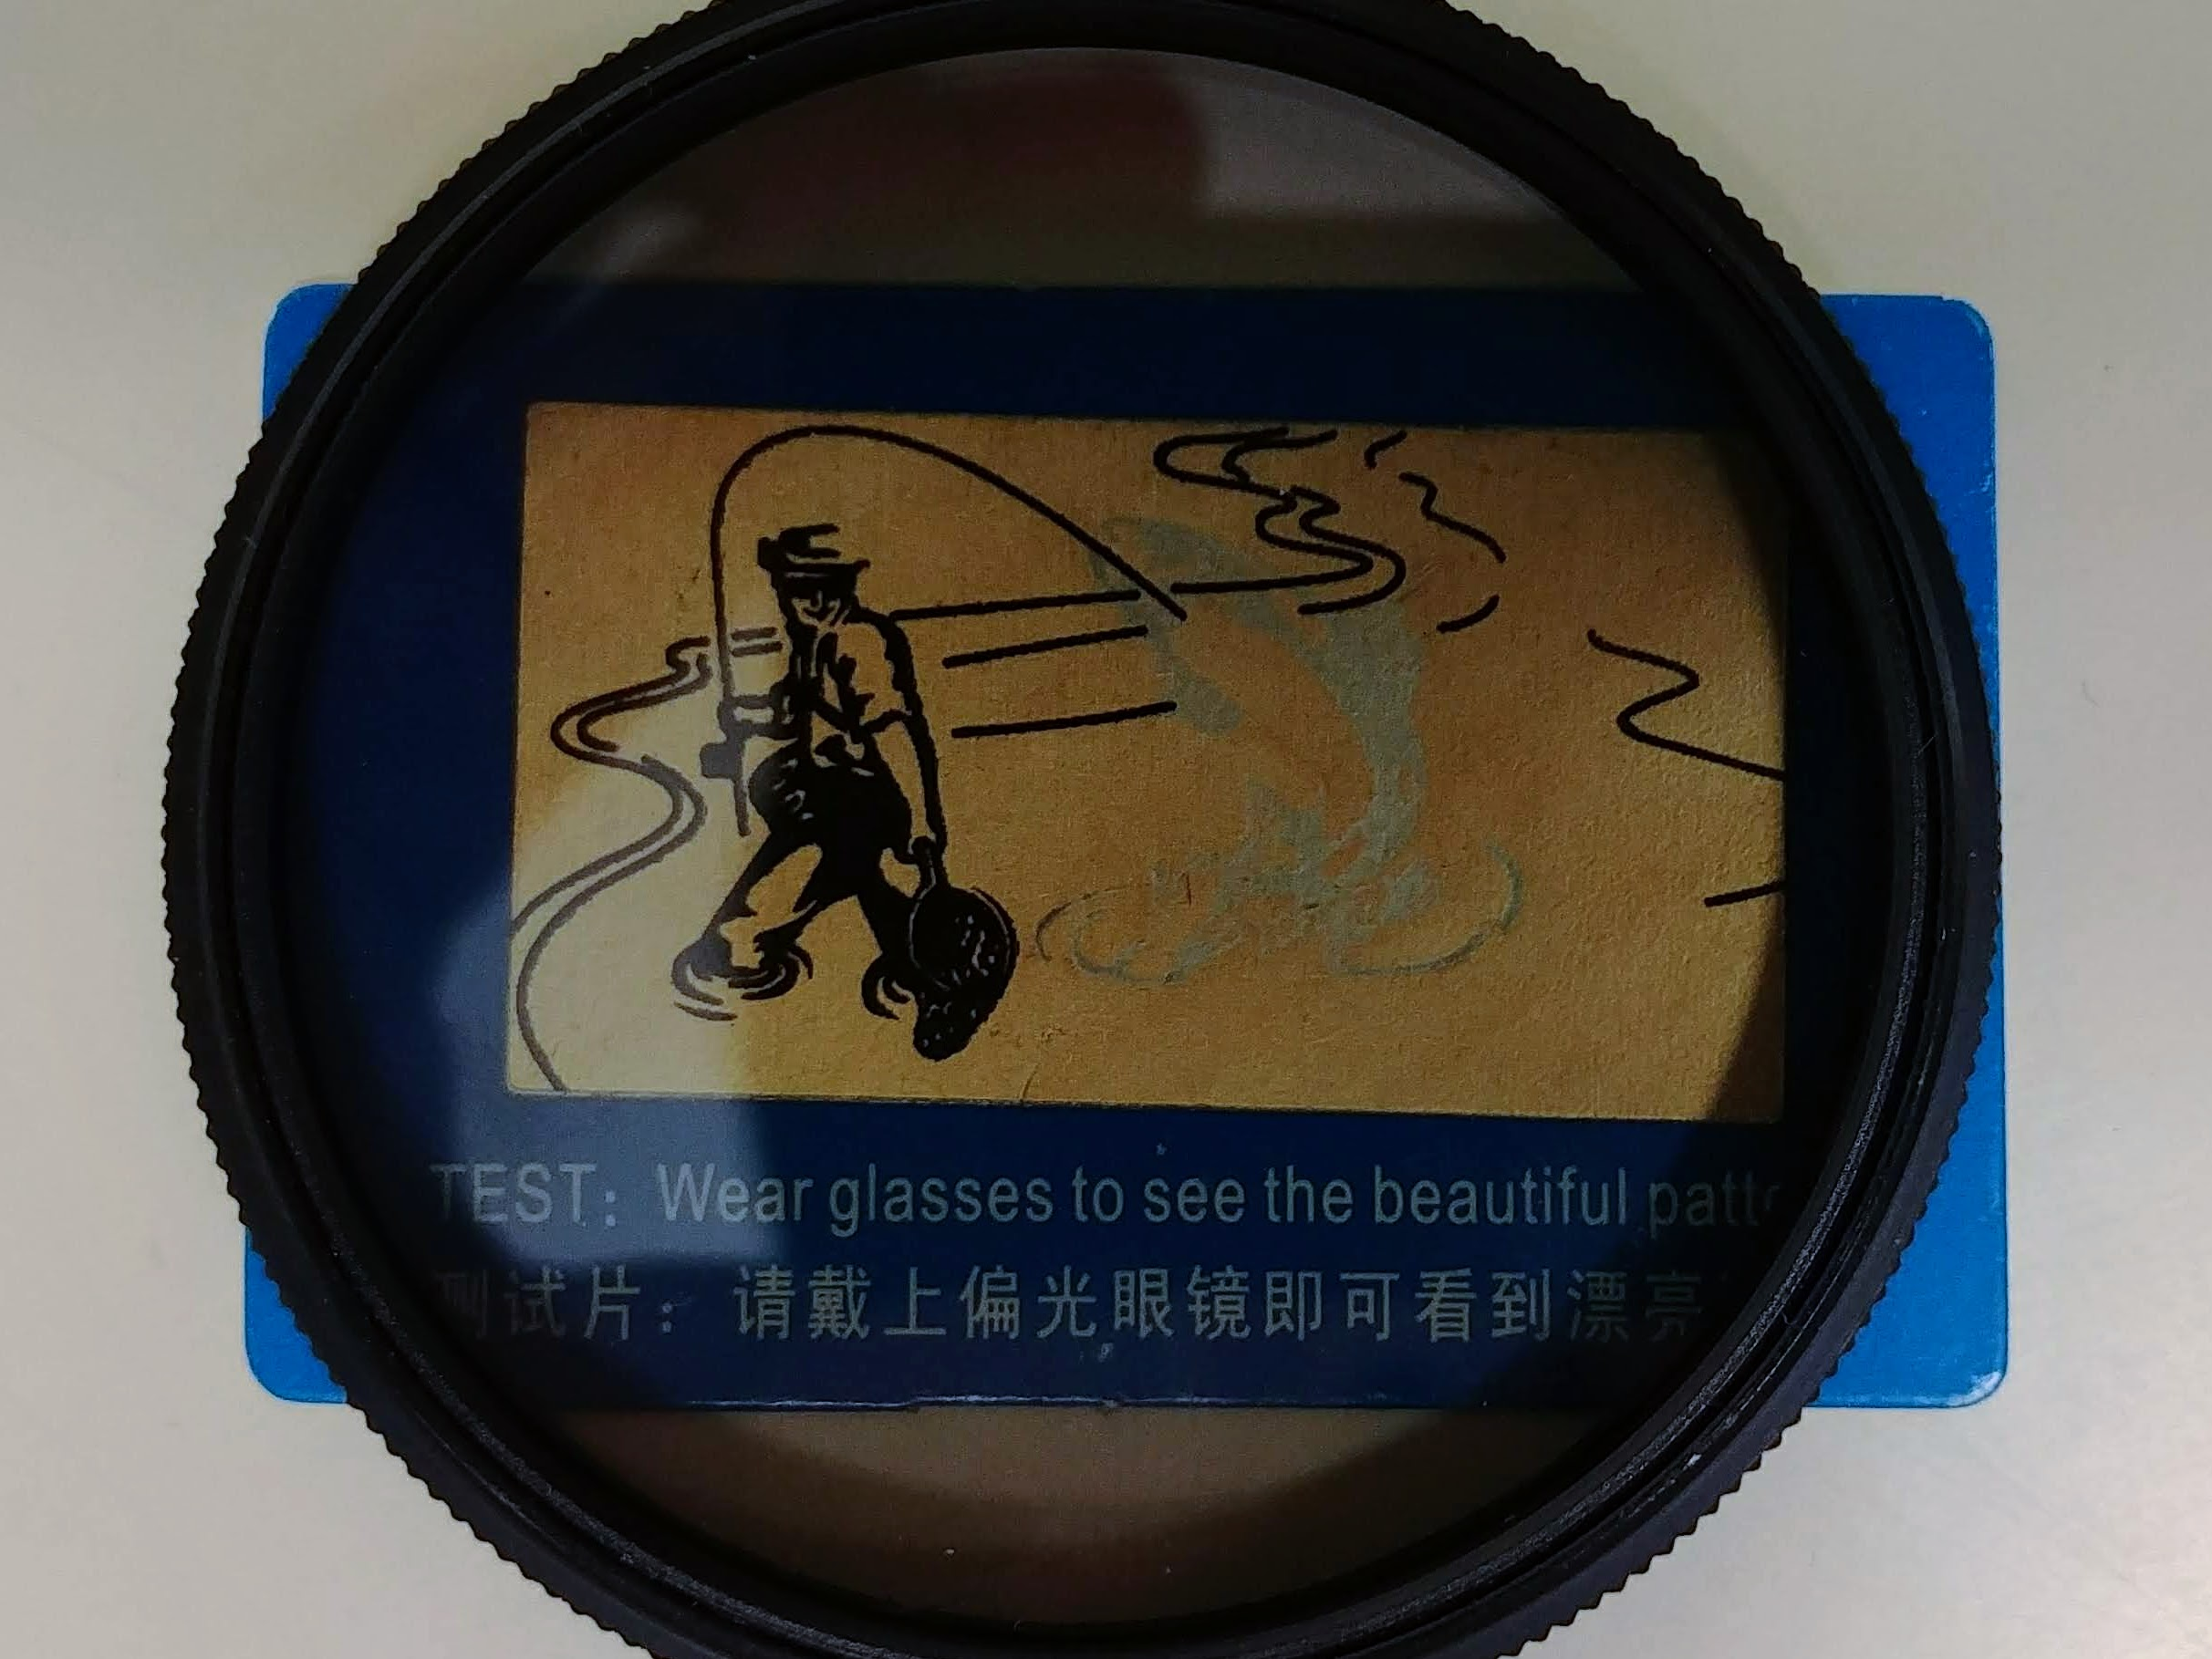
\includegraphics[width=.3\linewidth]{fig/experimentos/polarizacion_1}
	}\,
	\subfloat[$\phi = 45^\circ$]{
	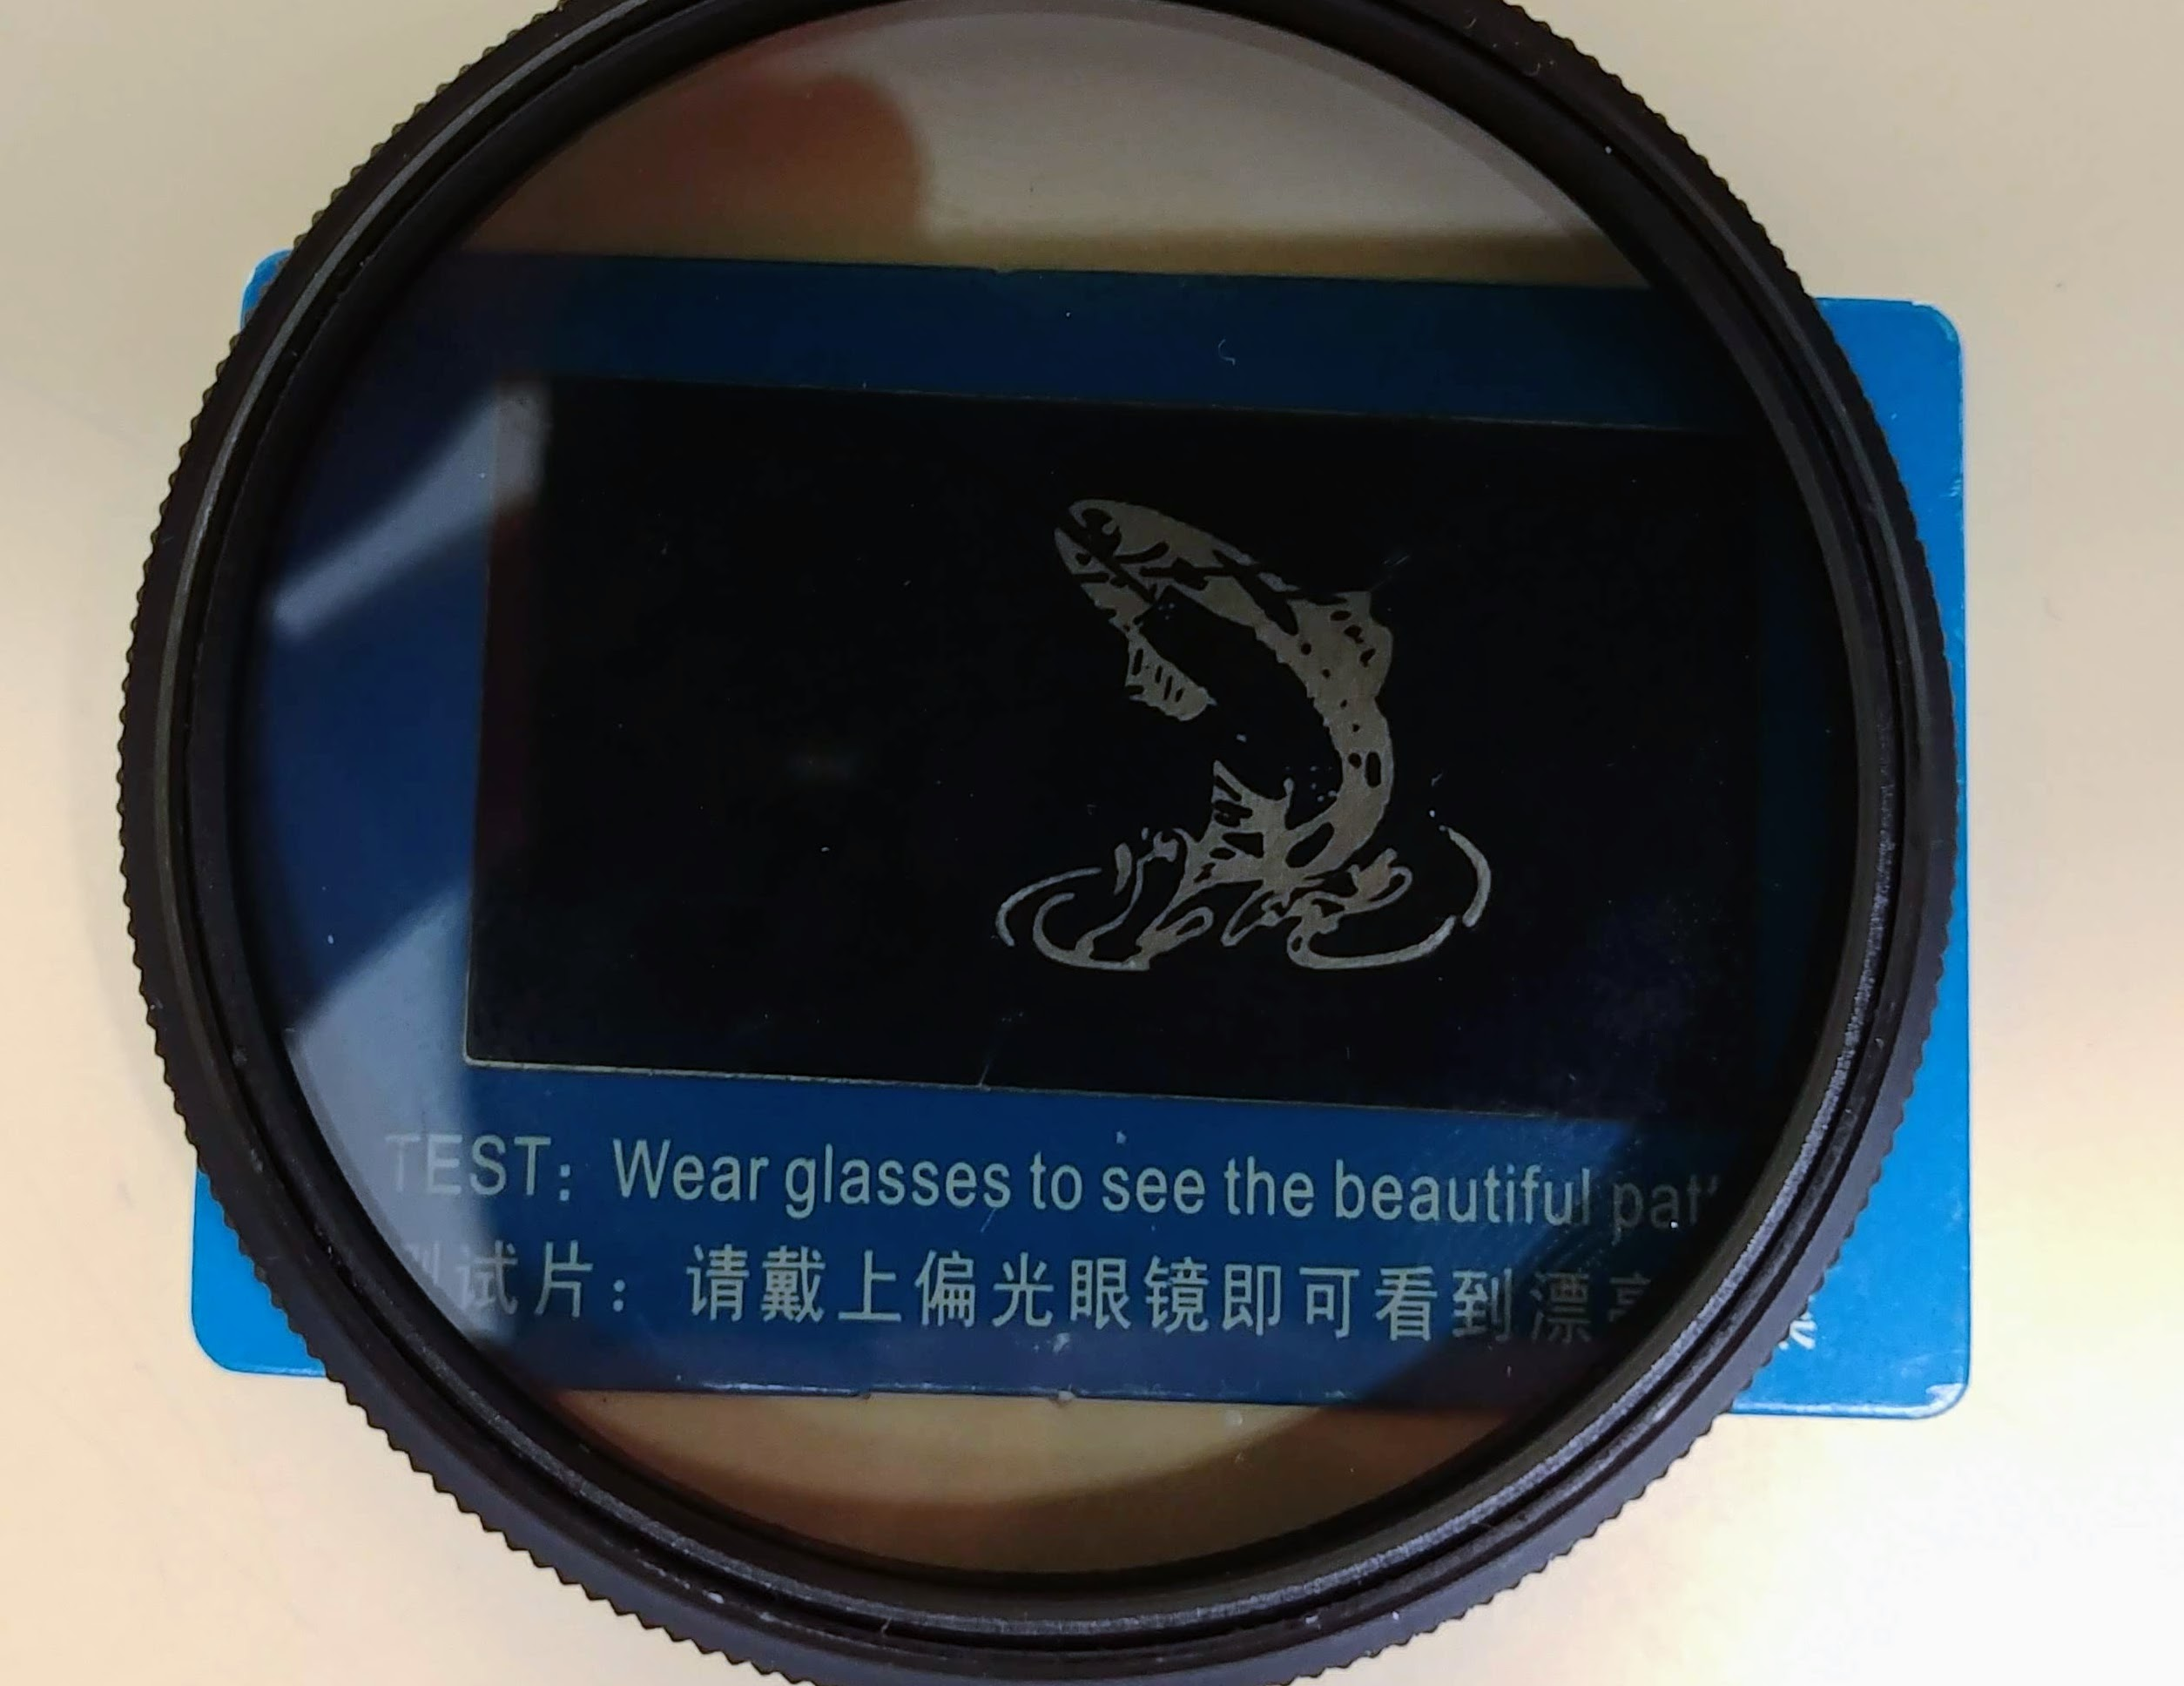
\includegraphics[width=.3\linewidth]{fig/experimentos/polarizacion_2}
	}\,
	\subfloat[$\phi = 90^\circ$]{
	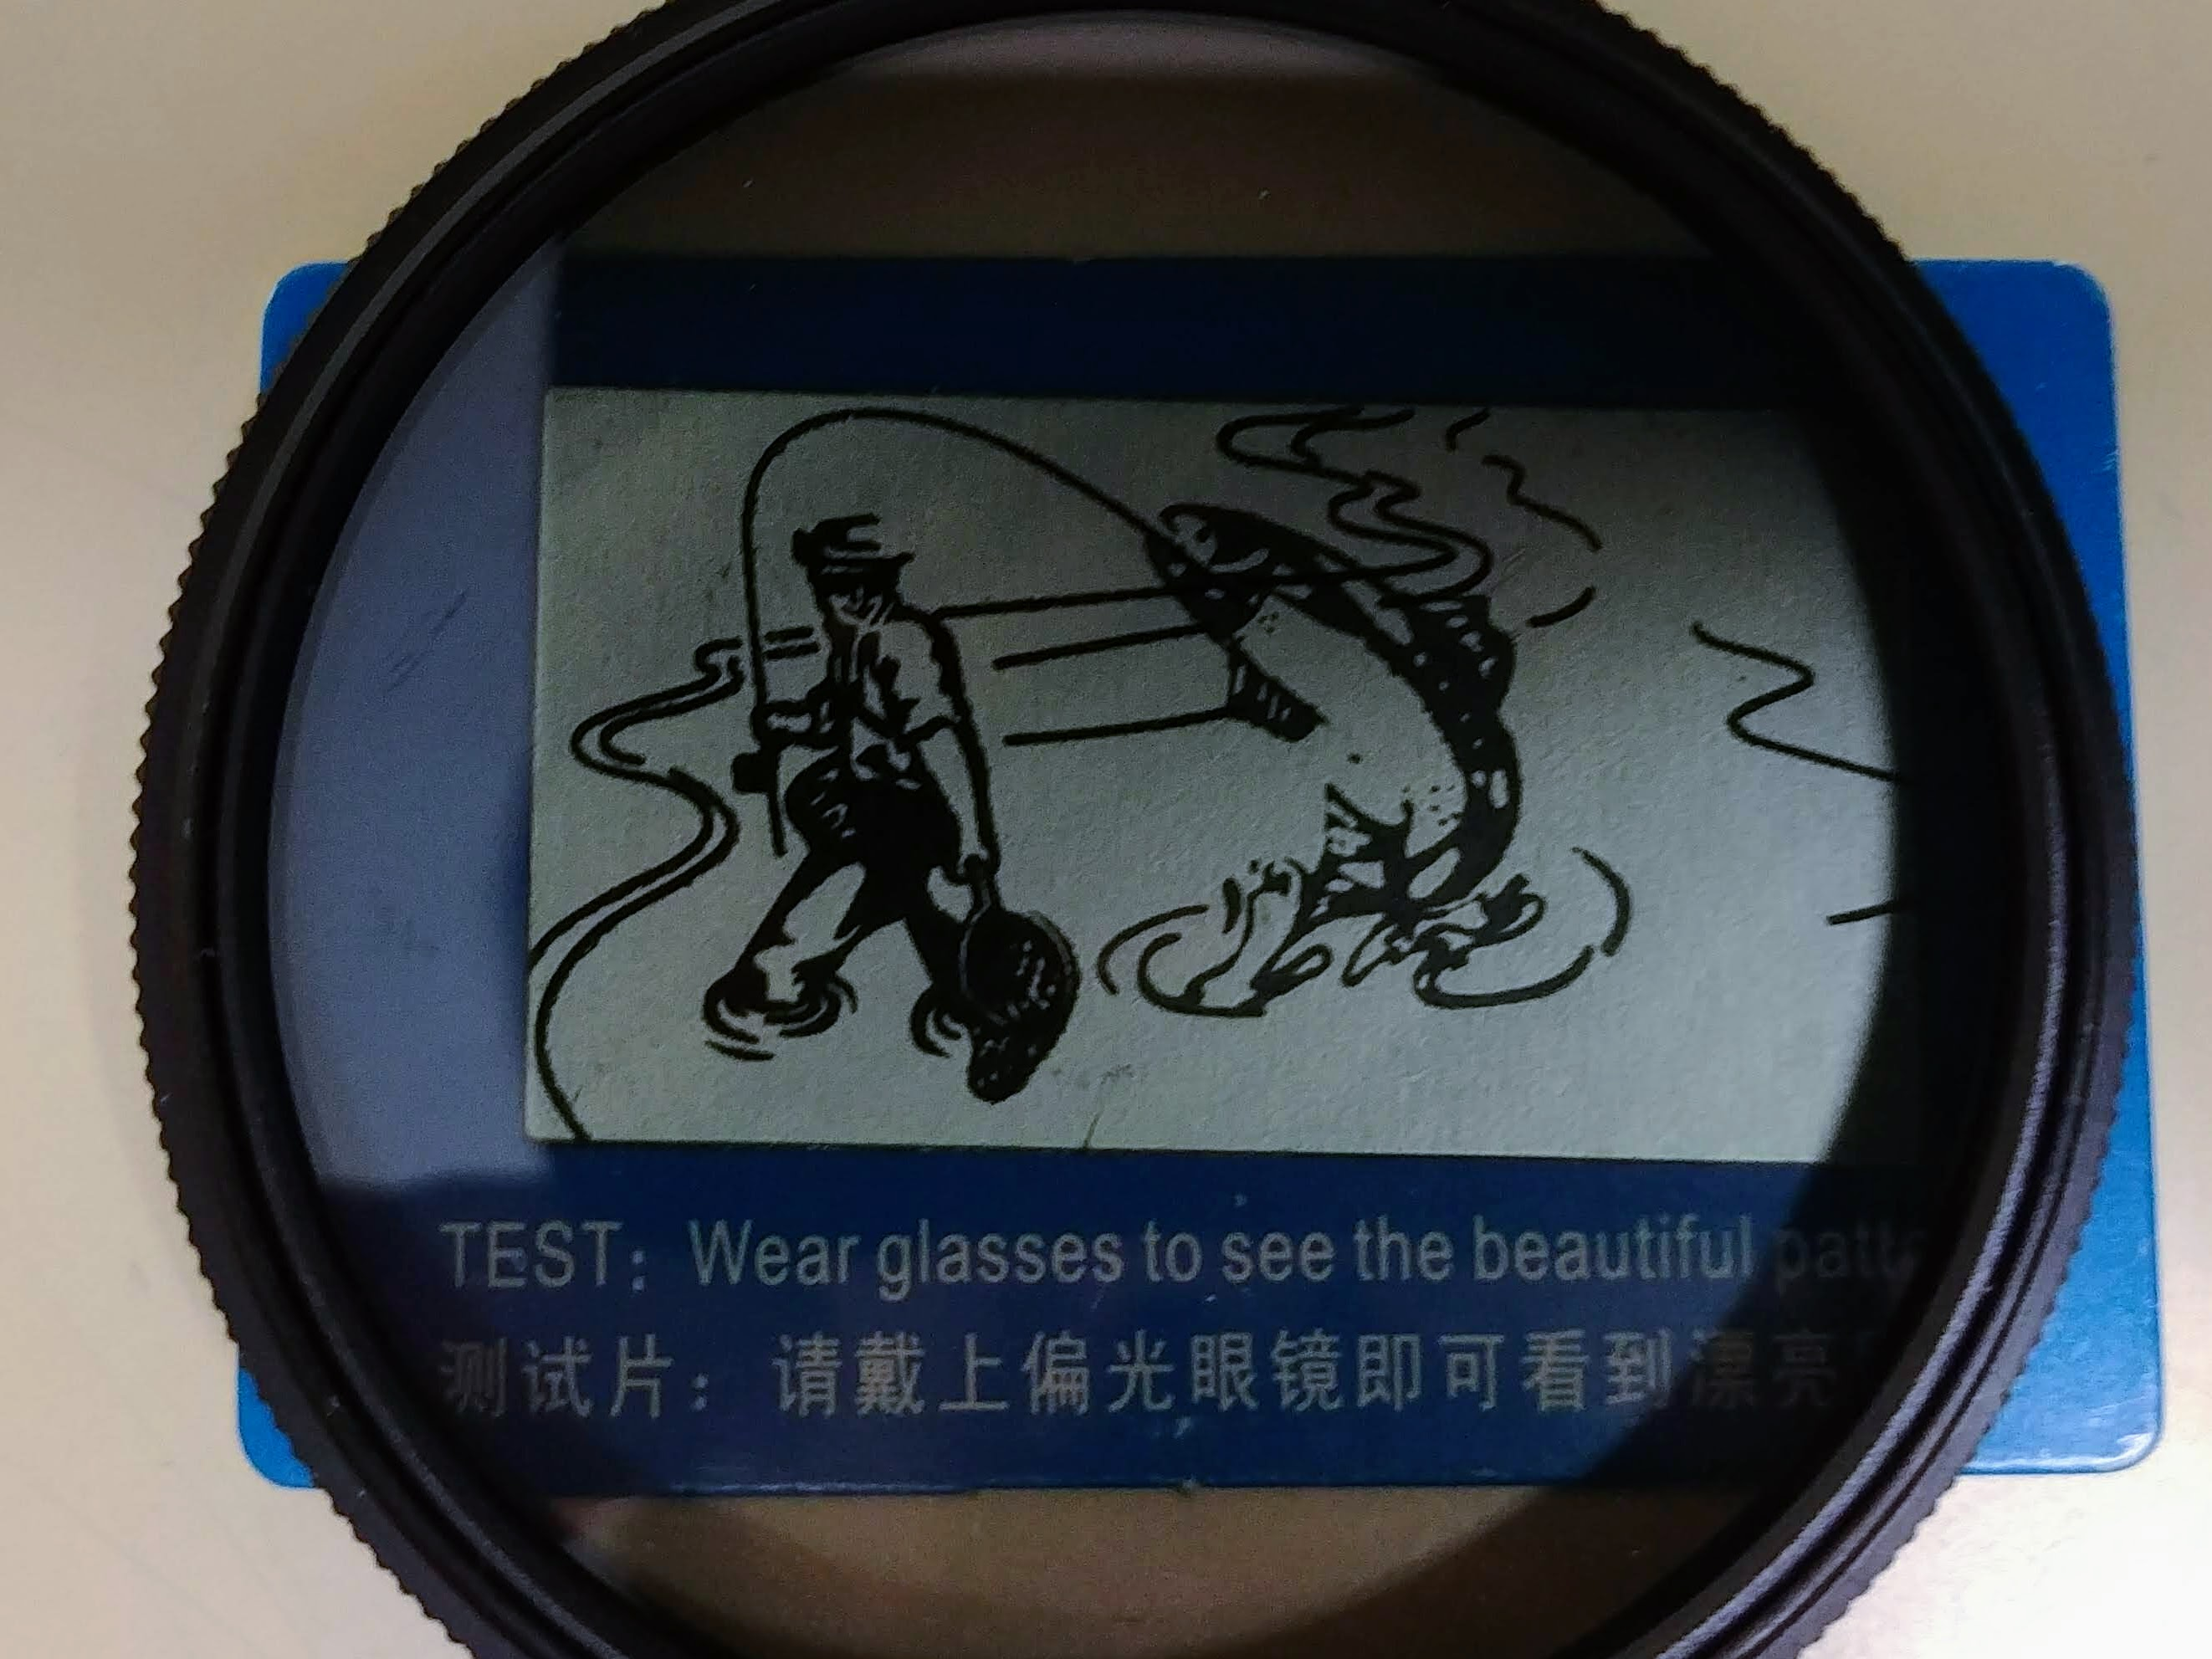
\includegraphics[width=.3\linewidth]{fig/experimentos/polarizacion_3}
	}
	\caption{\justifying Alguno objetos están diseñados para reflejar luz polarizada. Al ser pasada por un filtro polarizador podemos ver distintas imágenes según el ángulo que forma el eje de polarización del filtro con la luz polarizada reflejada.}
\end{figure}
\end{frame}

\begin{frame}{Polarizacón por birrefringencia}
\begin{figure}
	\centering
	\subfloat[Desdoblamiento de imágenes.]{
		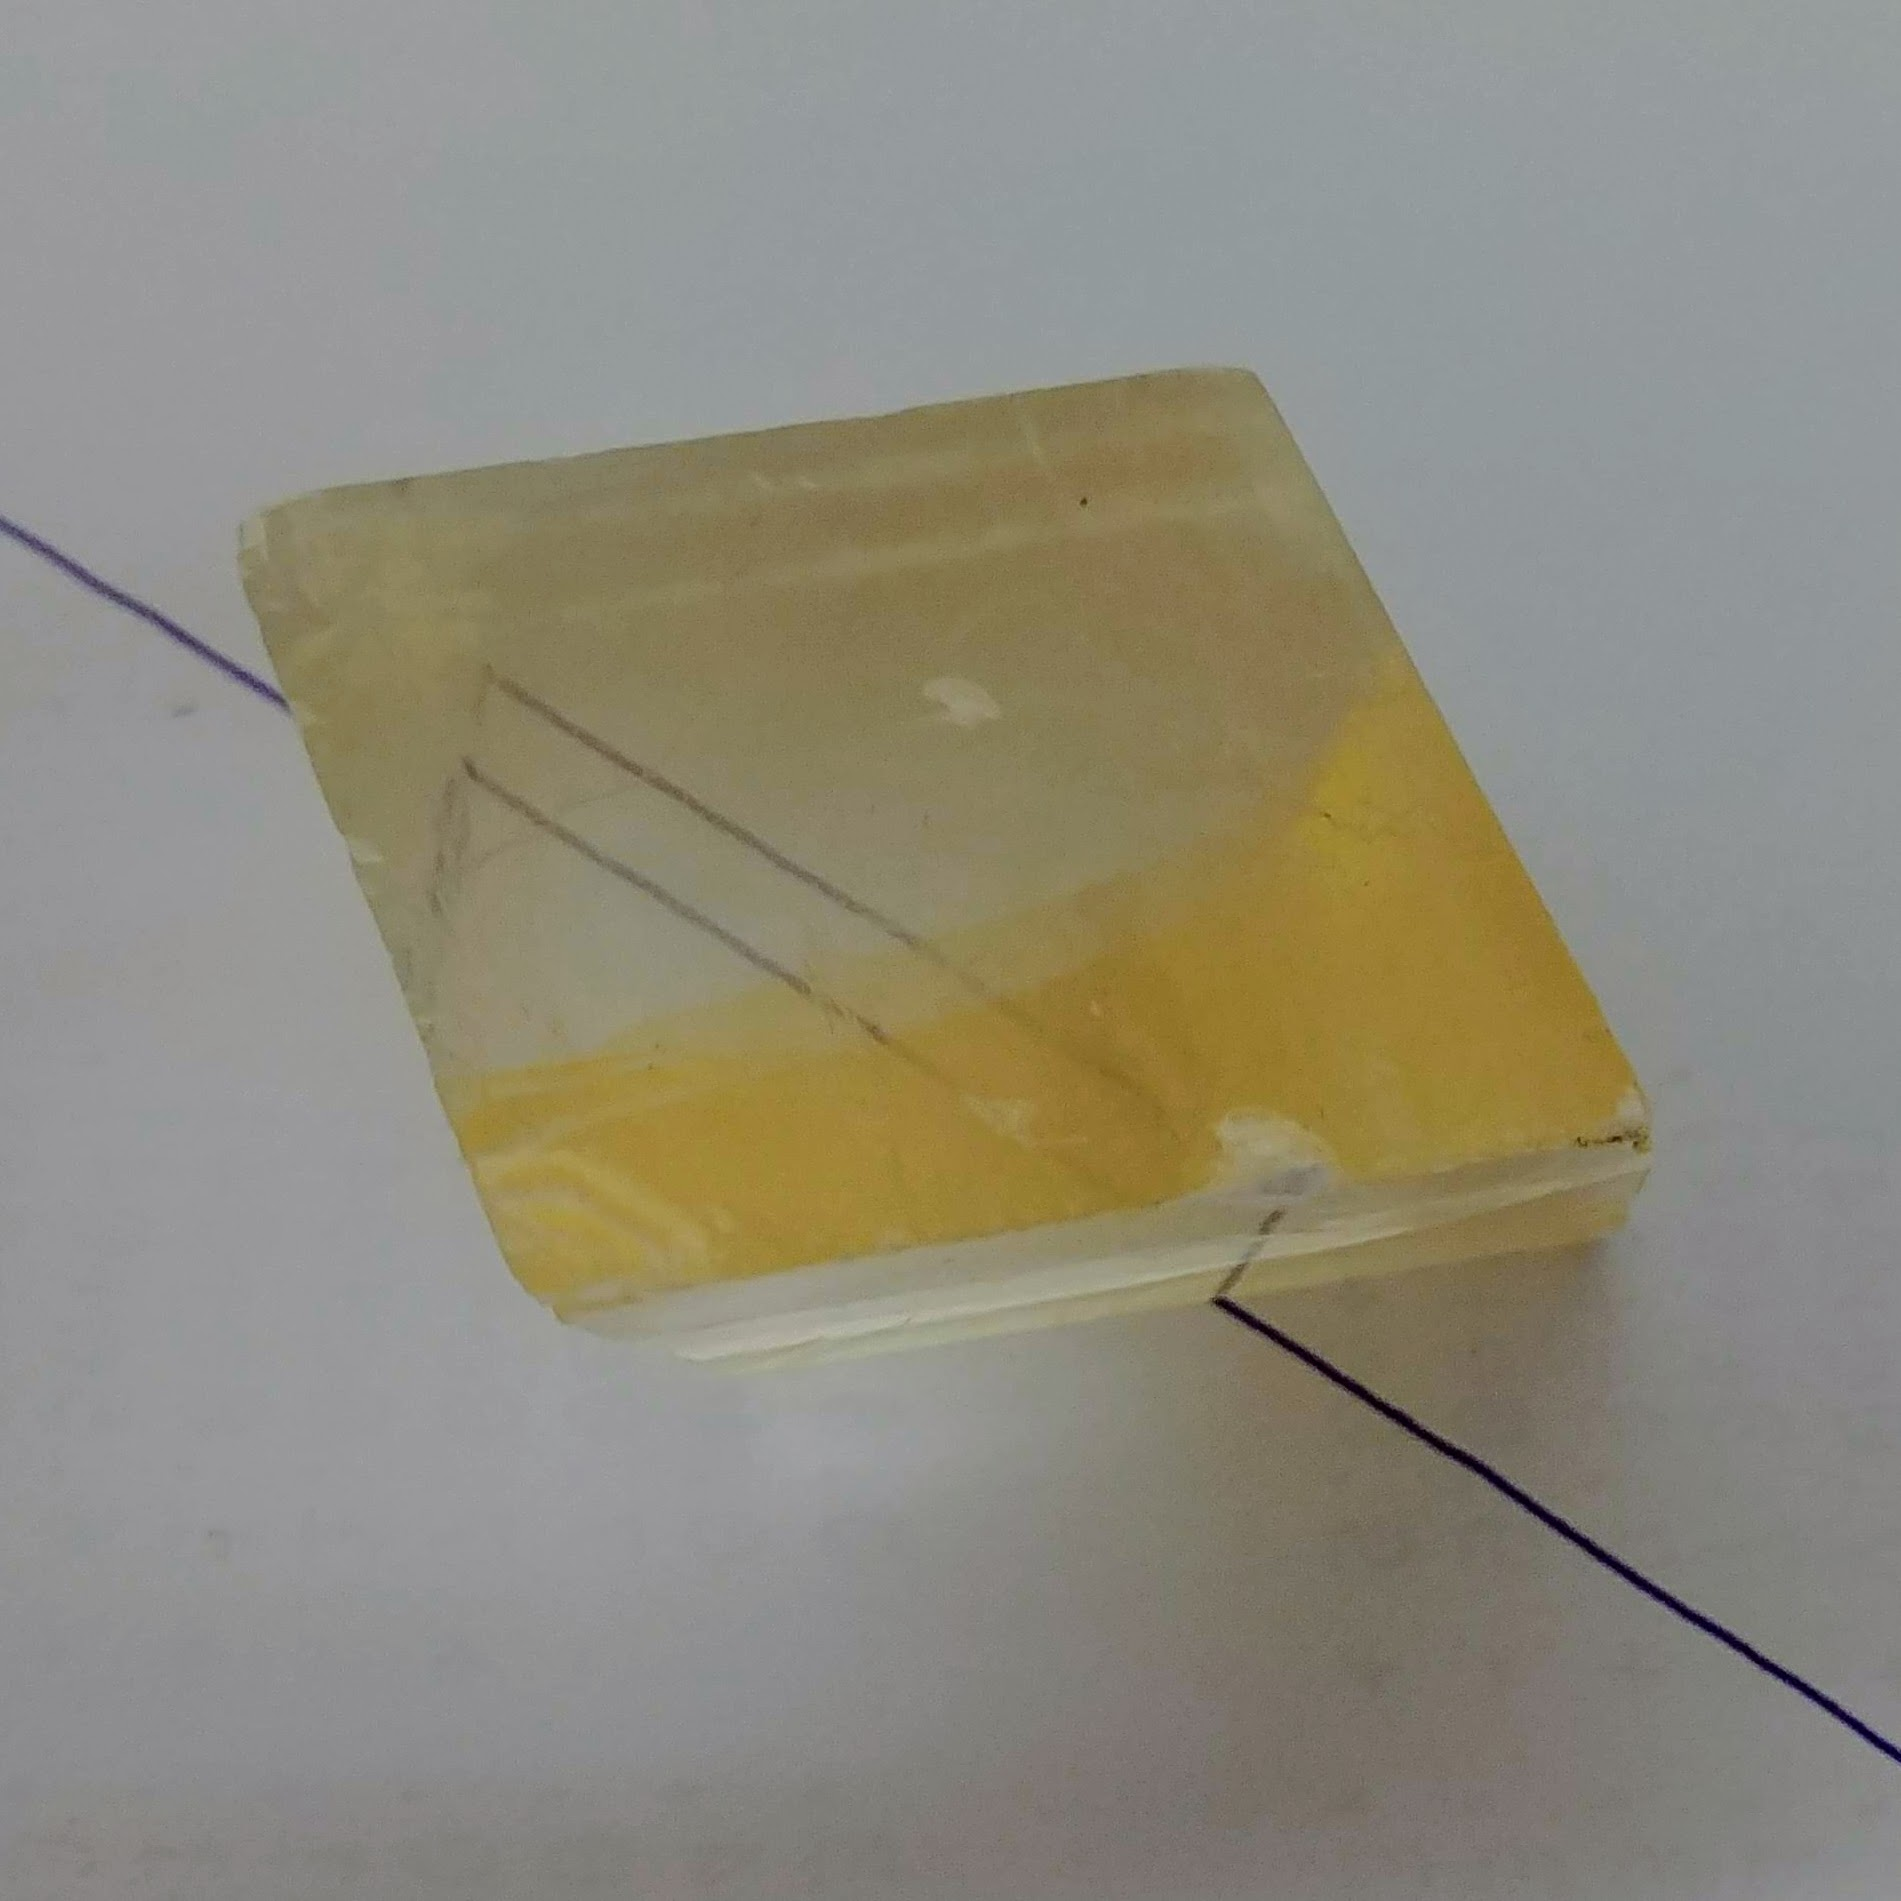
\includegraphics[width=.3\linewidth]{fig/experimentos/polarizacion_curazita}
	}\,
	\subfloat[Sólo la línea superior es visible.]{
		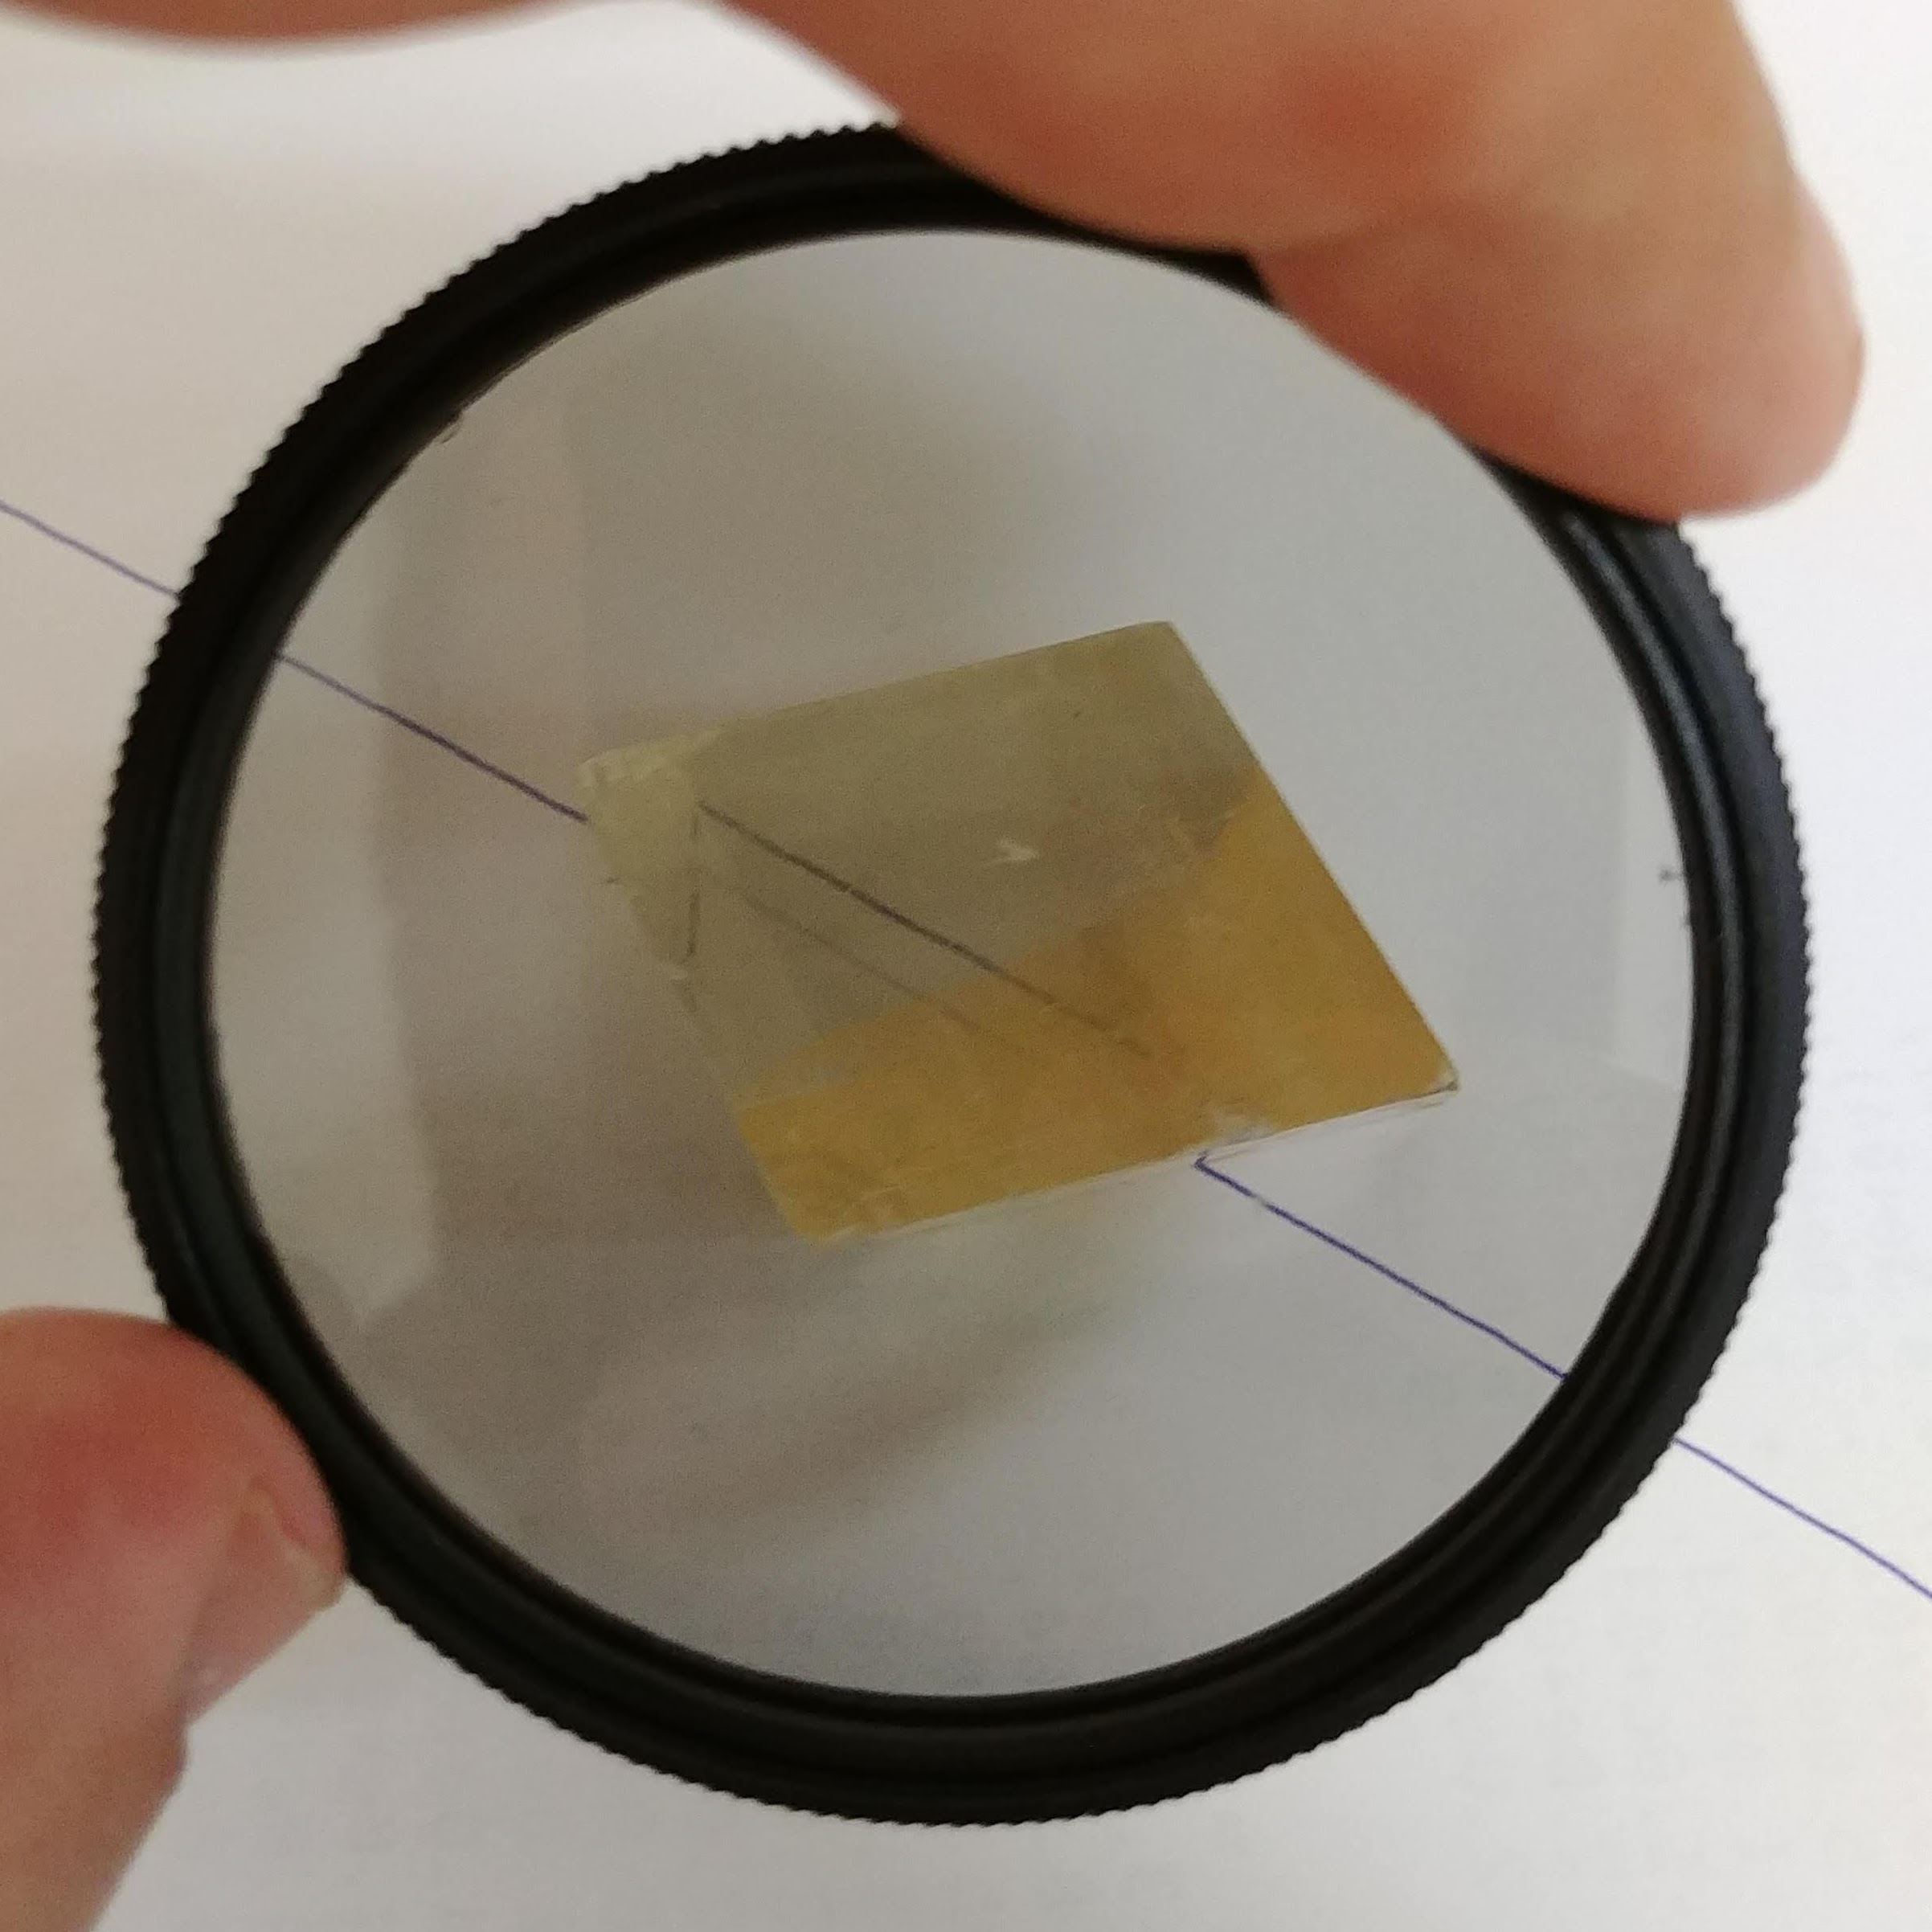
\includegraphics[width=.3\linewidth]{fig/experimentos/plarizacion_anisotropia_1}
	}\,
	\subfloat[Sólo la línea inferior es visible.]{
		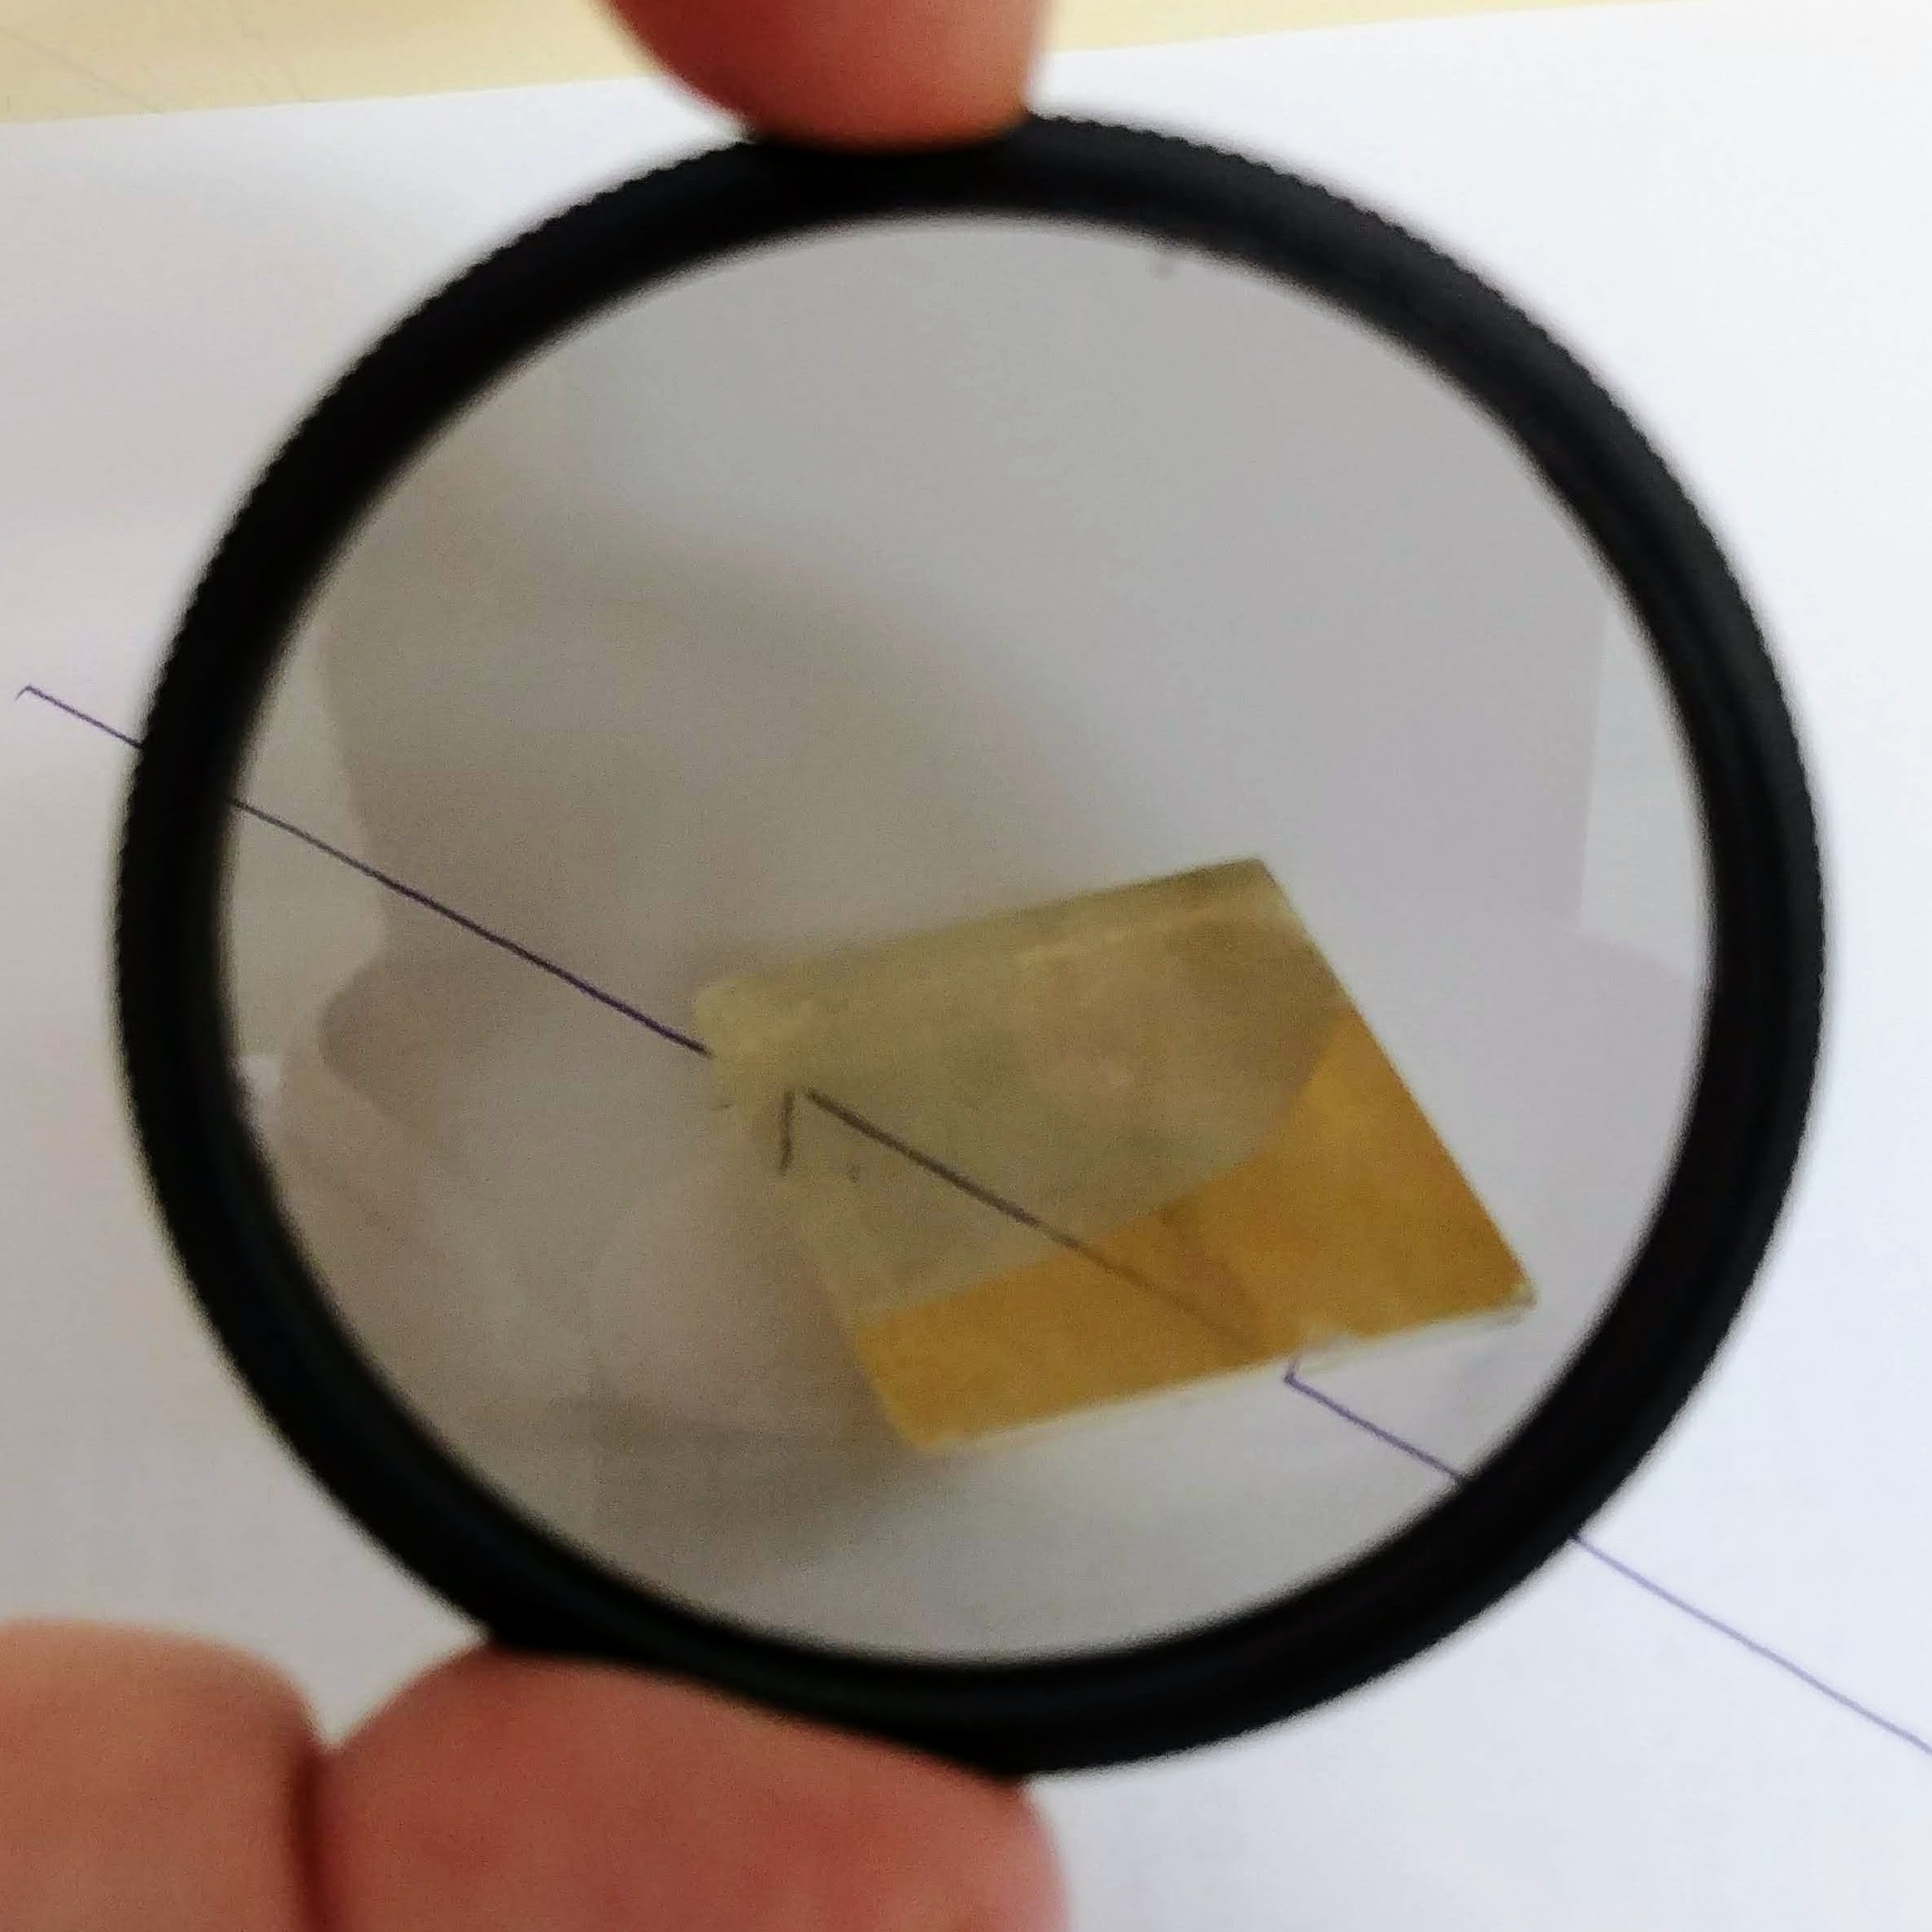
\includegraphics[width=.3\linewidth]{fig/experimentos/polariozacion_anisotropia_2}
	}
	\caption{\justifying Desdoblamiento de imágenes debido a la anisotropía del cristal de cuarzita. Al pasar la imágen desdoblada de la línea a través de un filtro polarizdor vemos que se verá una u otra imagen dependiendo de la posición del filtro. Por lo tanto, la luz que pasa a través de la cuarzita está polarizada.}
\end{figure}
\end{frame}

\begin{frame}<beamer:0>
  \bibliographystyle{plain}
  \IfFileExists{/home/luis/Documents/geg_library/library.bib}{
    \nobibliography{/home/luis/Documents/geg_library/library.bib}
  }{}
  \IfFileExists{C:/Users/lm/Documents/geg_library/library.bib}{
    \nobibliography{C:/Users/lm/Documents/geg_library/library.bib} 
  }{}
  \IfFileExists{E:/geg_library/library.bib}{
    \nobibliography{E:/geg_library/library.bib}
  }{}
\end{frame}

\end{document}
